\documentclass[12pt]{extarticle}

%%%%%%%% CREATE DOCUMENT STRUCTURE %%%%%%%%
%% Language and font encodings
\usepackage[english]{babel}
\usepackage[utf8x]{inputenc}
\usepackage[T1]{fontenc}
%\usepackage{subfig}

%% Sets page size and margins
\usepackage[a4paper,top=3cm,bottom=2cm,left=2cm,right=2cm,marginparwidth=1.75cm]{geometry}

%% Useful packages
\usepackage{amsmath}
\usepackage{appendix}
\usepackage{apacite}
\usepackage[square,sort,comma,numbers]{natbib}
\usepackage{graphicx}
\usepackage[colorinlistoftodos]{todonotes}
\usepackage{caption}
\usepackage{gensymb}
\usepackage{subcaption}
\usepackage{hyperref}
\usepackage{url}
\usepackage[nottoc]{tocbibind}
\usepackage{apacite}
\usepackage{float}
\usepackage{titling} 
\usepackage{blindtext}
\usepackage[colorinlistoftodos]{todonotes}
\usepackage{xcolor}
\definecolor{darkgreen}{rgb}{0.0, 0.4, 0.0}

%%%%%%%% DOCUMENT %%%%%%%%
\begin{document}

%%%% Title Page
\begin{titlepage}

\newcommand{\HRule}{\rule{\linewidth}{0.5mm}} 							% horizontal line and its thickness
\center 
 
% University
\textsc{\LARGE Delft University of Technology}\\[1cm]

% Document info
\textsc{\Large Internship Report}\\[0.2cm]
\textsc{\large SET3822}\\[1cm] 										% Course Code
\HRule \\[0.8cm]
{ \huge \bfseries Direct Air Capture System}\\[0.7cm]								% Assignment
\HRule \\[2cm]
\large
\emph{Author:}\\
Nithin Thomas Jacob (4841344)\\[1.0cm]

\emph{Supervisors:}\\
\begin{table}[H]
\centering
\scalebox{1.2}{\begin{tabular}{cl}
Company Supervisor   & Ir. Jan van Kranendonk \\
TU Delft Supervisor & Prof. dr. ir. Wiebren de Jong \\
\end{tabular}}
\end{table}

% Author info
\emph{Project duration:}\\
September $2^{nd}$, 2019 - December $21^{st}$, 2019
\\[4cm]
\begin{figure}[H]
\centering
\begin{minipage}{.5\textwidth}
  \centering
  
\includegraphics[width=\linewidth]{images/TU_delft_logo.jpg}
\end{minipage}%
\begin{minipage}{.5\textwidth}
  \centering
  
\includegraphics[scale=0.15]{images/zef.png}
\end{minipage}
\end{figure}
\end{titlepage}

\tableofcontents

\newpage
\listoffigures

\listoftables


\newpage
\section*{Preface}

In this report, I have summarized the three and a half months of work I have done in Zero Emission Fuels B.V (ZEF) under the Direct Air Capture (DAC) System. The scope of my work involved the fabrication, design and controlling the DAC system as well. I have acquired new skills and learned how to use Fusion360 models for the PMMA sheets and 3D models, 3D printing using Ultimaker 3D printers for the DAC Distributor, Laser cutting of PMMA sheets for the DAC columns and Arduino coding to control the sensor systems and running the polyethylenimine (PEI) across the system. 
\bigbreak
\noindent
Zero Emission Fuels B.V is a Carbon Capture Utilization (CCU) company that manufactures a micro-plant that captures $CO_2$ using polyethylenimine (PEI) or Tetraethylenepentamine (TEPA). The captured $CO_2$ is the desorbed and separated and converted to high grade Methanol that can be used as chemical feed stock or as fuel. 
\bigbreak
\noindent
Firstly, I would like to thank the founders of ZEF B.V for the opportunity that they had given me and their constant encouragement to hustle. Mr. Hessel Jongebreur and Mr. Ulrich Starke who showed keen interest in project development and their continued enthusiasm always pushed myself. Finally, Mr. Jan van Kranendonk for his guidance throughout my internship and always gave valuable input on what ot do and what not to do. 
\bigbreak
\noindent
Secondly, I would like to thank my colleagues of the ZEF V team which made it a memorable and fun working experience. I could always count on them to ask for help whenever I needed it and to improve my work. 
\bigbreak
\noindent
Thirdly, I would like to also thank my TU Delft Internship Supervisor Prof. Wiebren de Jong for his guidance and support through my Internship under ZEF and readily accepted my internship application.  
\bigbreak
\noindent
Fourthly, a special mention to the faculty of SET Internship office for giving me this opportunity and work experience. With out their work and correspondence, this internship wouldn't have been possible. 
\bigbreak
\noindent
Finally, I would like to thank my friends, family for being understanding and supportive during my internship of these three and a half months


\newpage
\section{Introduction}
%Over the last decade how the CO2 levels have increased from 200 ppm to 400 ppm. 
%General overview of carbon emissions and climate accords.
It has come to the attention to most governmental bodies and general public that the threat of global warming is real. It is also noted that this year most countries recorded their highest ever temperature records for example, this year's July $25^{th}$ marked the hottest ever since the first recorded temperature at 1901 in the Netherlands \cite{Pieters2019}. According to Allen et al., the $CO_2$ emissions into the atmosphere is estimated to be over 3.67 trillion tones of $CO_2$, this will cause a carbon dioxide caused warming of 2 \degree C above the pre-industrial temperatures by 2500 \cite{Allen2009}. $CO_2$ direct air capture or DAC is growing interest in research and development in order to fight climate change. There is two types of DAC systems at the moment. High temperature solid sorbent (HT DAC) systems that operate at about 800 - 900 \degree C using carbonates or Sodium tri - titanante. The second type is low temperature solid (LT DAC) system that operate at temperature ranges from 80 to 120 \degree C using polyamines \cite{Fasihi2019}.

\subsection{Low temperature solution DAC}
\noindent
In order to address the growing concerns of carbon emissions and global warming. The people at Zero Emission Fuels B.V (ZEF) are trying to make a micro-plant that is capable of capturing $CO_2$ from the atmosphere and converting into industry grade (AA grade) methanol that can used as fuel or chemical feedstock. The plant is powered by photo-voltaic solar power which reduces the carbon footprint even more. The energy is utilized in the Alkaline electrolysis cell (AEC) that produces $H_2$, which reacts with $CO_2$ and makes methanol ($CH_{3}OH$) and to run the pumps and compressors across the micro-plant. At ZEF, we work with polyamines and hence, the DAC system used is a low temperature sorbent solution using PEI or TEPA. 

\begin{figure}[H]
    \centering
    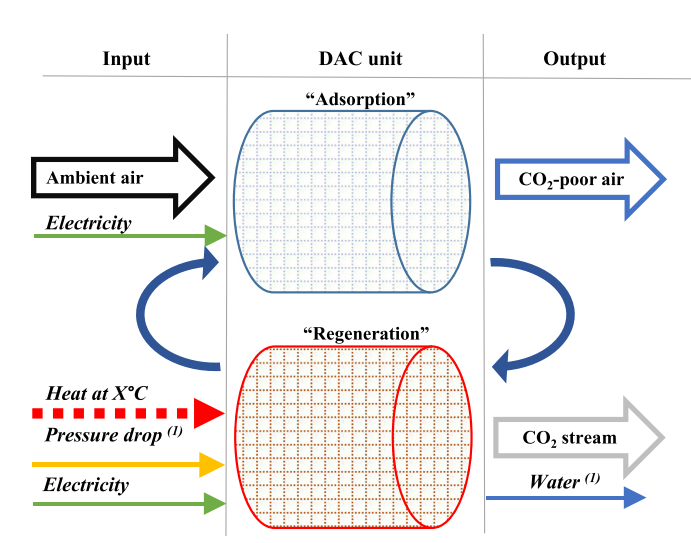
\includegraphics[scale = 0.6]{images/LT_DAC.png}
    \caption{Low temperature solution DAC system}
    \label{fig:LTDAC}
\end{figure}

\noindent
In Figure \ref{fig:LTDAC} above, an example of a LT DAC system can be seen and based on this model. Fasihi et al. talks about all kinds of DAC systems that are available at present and has given a economic analysis of each system based on DAC companies that are working at present such as Climeworks, Carbon Engineering, Antecy, etc. However, I shall limit the discussion to LT DAC systems as the DAC system that is present in ZEF is a LT DAC system. 


% Table generated by Excel2LaTeX from sheet 'Sheet1'
\begin{table}[htbp]
  \centering
  \caption{LT DAC specifications \cite{Fasihi2019}}
  \tiny{
    \begin{tabular}{|l|c|c|c|c|c|c|c|c|c|c|}
    \hline
    \textbf{Sorbent} & \textbf{$CO_2$ conc.} & \textbf{adsorption} & \multicolumn{2}{c|}{\textbf{desorption}} & \multicolumn{3}{c|}{\textbf{energy demand}} & \multicolumn{2}{c|}{\textbf{cooling }} & \textbf{$CO_{2}$ purity} \\
    \hline
          &       & T     & T     & P     &       &       & by    & T     &       &  \\
    \hline
       Units   & ppm   & \degree C & \degree C & bar   & $kWh_{el}/t$ & $kWh_{he}/t$ &       & \degree C &      & \%  \\
    \hline
    amine-based & 400   & ambient & 100   & 0.2   & 200-300 & 1500-2000 & waste heat & 15    & air/water & 99.9 \\
    \hline
    amino-polymer & 400   & ambient & 85-95  & 0.5-0.9 & 150-260 & 1170-1410 & steam & ambient & water evaporation & >98.5 \\
    \hline
    TRI-PE-MCM-41 & 400   & ambient & 110   & 1.4   & 218   & 1656  & steam & -    & -    & 88 \\
    \hline
    MOF (Cr) & 400   & ambient & 135-480 & 1     & 1420  &    -   & HT steam & -    & -    & - \\
    \hline
    MOF (MG) & 400   & ambient & 135-480 & 1     & 997   &    -   & HT steam  & -    & -    & - \\
    \hline
    $K_{2}CO_{3}$/$Y_{2}O_{3}$ & 400   & ambient & 150-250 & -    &    -   &    -   & el. Heater & -    & -    & - \\
    \hline
    $K_{2}CO_{3}$ & -    & ambient & 80-100 & -    & 694   & 2083  & waste heat & ambient & airflow & - \\
    \hline
    \end{tabular}%
    }
  \label{tab:ltdac}%
\end{table}%

\noindent
In Table \ref{tab:ltdac}, it can be seen that amine - based sorbent DAC systems has the maximum $CO_2$ purity based on literature \cite{Fasihi2019}. Compared to ZEF's competitors like Antecy in Netherlands and Climeworks in Switzerland, who use waste heat from industries to heat their desorption units and only store the carbon in these amines. ZEF has the upperhand and aim to bring the price down to 40 euros per ton of $CO_2$ captured by relying on solar energy to provide the process energy required to run the microplant. The cost is further brought down as ZEF conducts methanol synthesis using the absorbed $CO_2$ to AA grade methanol that can be used as alternative fuels. Thereby making it a completely carbon negative carbon capture utilization system. According to Fasihi et al., the cost of LT DAC systems can drop to potentially event 32 euros / ton of $CO_2$ in the year 2050. Unlike its DAC competitors who absorb $CO_2$ from high carbondioxide emission industries only, ZEF captures $CO_2$ directly from the atmosphere.  


\subsection{Report overview}

In this report we will see the scope of my internship and what I had done with my time at Zero Emission Fuels B.V. I cover a section on previous work done on the Direct Air Capture system in Zero Emission Fuels B.V that laid a foundation on what I should do and on what I should improve on in Section \ref{sec:prework}. In Section \ref{sec:mywork}, I cover what I did in the span of my internship. The internship was divided in the form of Sprints which is periods of 3 weeks, hence the whole internship contains 5 Sprints in total. I have described what I have done in each Sprint from Section \ref{sec:sprint1} to Section \ref{sec:sprint5}. In Section \ref{sec:results} contains the main observations made from running the DAC systems. Based on the findings from Section \ref{sec:results}, I have written the discussion of results in Section \ref{sec:results}. I have made some suggestions for the next Direct Air Capture team of ZEF VI in Section \ref{sec:recom} and added concluded the report in Section \ref{sec:conc}

\newpage
\section{The old DAC Systems}
\label{sec:prework}

In this section, I shall summarize the works done previously by Zero Emission Fuels B.V relating to the Direct Air Capture System (DAC). Before starting my work at the internship in the ZEF V team. I have to read and learn what was already worked on by the previous interns and thesis students. So that, I can get an idea in-order to know what has been done, what works and to know what can be done further. The section with be divided into various subsections starting from ZEF I to ZEF IV. In each of the subsections, the work done by them and their findings shall be elaborated further. 

\subsection{ZEF I - the beginning}

According to the internship report submitted by Sjors and Sotiris \cite{Wagenaar2018}. The first DAC team realized that going about physical swing adsorption won't be feasible due to the low concentration of $CO_2$ in the atmosphere and flue gases is only about 10 - 15\% of the exhaust gases and moisture inhibits the kinetics for physical adsorbent. They also defined what are the characteristics required to be full-filled in finding the candidate adsorbent which was having :-

\begin{itemize}
    \item High adsorption capacity
    \item High kinetics 
    \item Chemical and Thermal stability
    \item Low cost 
    \item Fouling resistance 
    \item No promotion of unwanted by-products
\end{itemize}

On further literature study, it was determined that most accepted study is the Impregnation of Polyethylenemeine (PEI) on mesoporous silica. It was also determined that the adsorbent must be heated to 120 \degree C  in-order to desorb the $CO_2$. \textbf{Note:} It is critical to note that PEI in combination with $O_2$ at high temperatures (around 120 \degree C) causes sorbent degradation. 

\subsubsection{Design}
The input feedstock for the ZEF plant is 187 grams of $CO_2$ in 8 batches (batch process). A container of 3L capacity was 3D printed using PLA material and various kinetics studies were conducted to determine the adsorption and desorption characteristics of PEI. The DAC column is chosen to be a packed bed reactor as there seems to be a lot of design issues with multiple layer fluidized bed system. The reactor bed was 3D printed using Polycarbonate (PC) material as it is the only material that can withstand the sorbent heating to 120 \degree C for desorption. The absorption and desorption of $CO_2$ is going to be taking place simultaneously in 2 seperate chambers which can be seen more elaborately in Figure \ref{fig:zef1ads} and Figure \ref{fig:zef1des} and in Figure \ref{fig:zef1ass} we can see the isometric view of the DAC unit that was designed and fabricated by the ZEF I team. 

\begin{figure}[H]
\centering
\begin{minipage}{.5\textwidth}
  \centering
  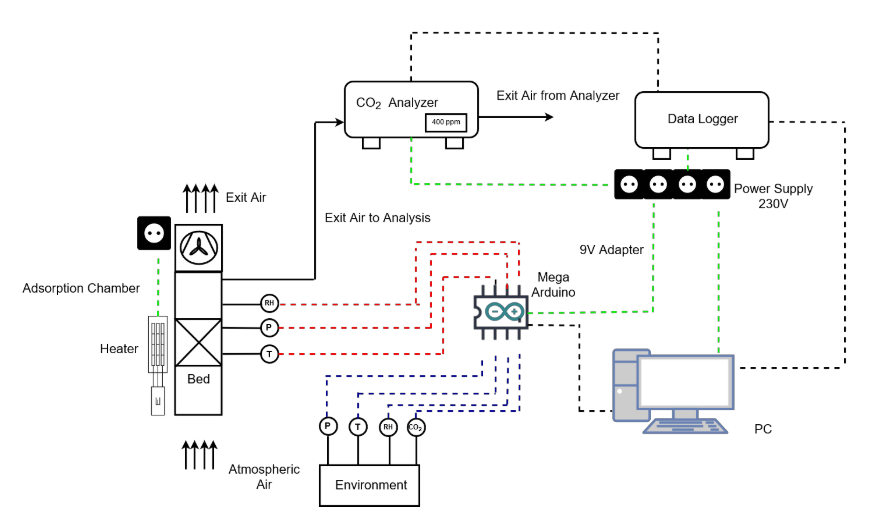
\includegraphics[width=\linewidth]{images/previouswork/zef1ads.png}
  \captionof{figure}{Schema of adsorption process \cite{Wagenaar2018}}
  \label{fig:zef1ads}
\end{minipage}%
\begin{minipage}{.5\textwidth}
  \centering
  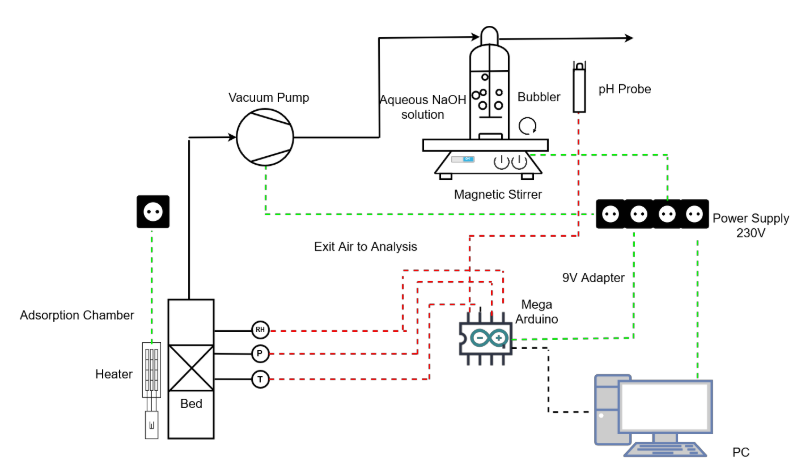
\includegraphics[width=\linewidth]{images/previouswork/zef1des.png}
  \captionof{figure}{Schema of desportion process \cite{Wagenaar2018}}
  \label{fig:zef1des}
\end{minipage}
\end{figure}

\begin{figure}[H]
    \centering
    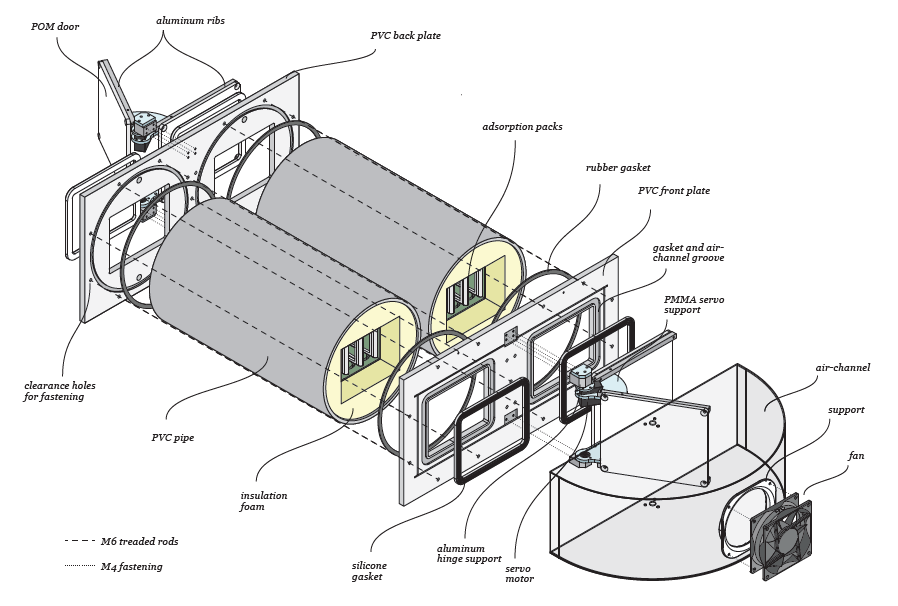
\includegraphics[width=\linewidth]{images/previouswork/zef1ass.png}
    \caption{Isometric view of the DAC unit assembly \cite{Azzalini2018}}
    \label{fig:zef1ass}
\end{figure}

\subsubsection{Further work}
The DAC team of ZEF 1 got a DAC system running from scratch. However, the heating and cooling systems were not installed. Hence, no system testing could be performed. Some of the relevant conclusions and recommendations put forward by the team was :

\begin{itemize}
    \item In order to address the fluctuations in sensor readings. Powering the sensors using a stable and constant 9V power adapter is required. 
    \item Selection of a cheaper sorbent material such as amine grafter sugarcane bagasse. 
    \item Since PEI is a non - newtonian fluid, higher $CO_2$ absorption might be observed in order to optimize the parameter. 
    \item Innovative designs might help in better heat utilization for the other sub-systems and can aid in the adsorption of $CO_2$ in DAC. 
    \item Testing with the heating and condensation units must be carried out. 
\end{itemize}

\subsection{ZEF II - the shift to monoliths}

During the time of ZEF II, the DAC system was still in a design phase and it was suggested by R. Berg to shift to monoliths in his MSc thesis report. His goal was to come up with a DAC system design that can be mass produced at a reasonable price. At this stage, ZEF still considered that batch process is the best way to approach DAC system as well. The reasons why he suggested this DAC system are \cite{Berg2018}: 
\begin{enumerate}
    \item Small size - can be mass produced easiliy and makes handling easier 
    \item Heat integration - allows heating using Peltier elements
    \item Functionality
    \item Exchangeable monolith
    \item Stand alone DAC - easily integrated with other systems. 
    \item Capture - captures $CO_2$ and water vapor. 
    \item Lower capture costs - R. Berg estimates $CO_2$ capture costs to about 123 euros per ton $CO_2$
\end{enumerate}

There were also students who had to study the $CO_2$ loading characteristics in PEI 10K and 1.2K to find the best candidate that could work best in the DAC system by studying the amount of $CO_2$ absorbed in the PEI. It was found that 10K PEI has slower kinetics than 1.2K PEI but absorbs less water compared to 1.2K. It was also found that active carbon is highly insulating and heating is slow. Thereby we have large heat demand for the desorbtion system which is very undesirable \cite{Laake2018}. This is where the shift from batch processing to continuous DAC system happened for ZEF. 


\subsection{ZEF III - continuous DAC system studies}

In order to study the feasibility of a continuous DAC system, the interns of ZEF III conducted various test farms to let PEI flow through and observations were made of the flow of PEI through the channels that were 3D printed. According to M. Sinha, these are the following observations made during the testing phase \cite{Sinha2018} : 

\subsubsection{Absorption}

\begin{enumerate}
    \item As the PEI layer goes down, the PEI stays more time on the plate and can absorb more $CO_2$ per kg of amine. A layer thickness of about 0.1 mm was recommended. 
    \item Direction of airflow has no effect on the amount of $CO_2$ absorbed by the sorbent. 
    \item Paper as a flow surface is found to have the lowest layer thickness, which is desired as elaborated in the first point. 
    \item Pre-wetting the flow surface is very essential to achieve a very good flow
    \item A honey comb structure must be used at the entry of the sorbent inorder to reduce surface tension effects. 
\end{enumerate}

\subsubsection{Desportion}

\begin{enumerate}
    \item Reaction of PEI and TEPA with metals s
    \item PEI600 and PEI1200 burning at 145 \degree C. 
    \item Proper enclosure must be ensured inorder to remove water vapor from the system. 
    \item Within 6 minutes, 80\% of the absorbed $CO_2$ could be desorbed in the desorption chamber. 
\end{enumerate}

Some of the recommendations given by M. Sinha were to study more on the flow of air as well and the difference a laminar or turbulent flow can make with $CO_2$ absorption. Study on the viscosity changes were also recommended to understand the flow of PEI better. Life cycle and mass transfer kinetics during the desorbtion process was also recommended.   



\subsection{ZEF IV - absorption \& desorbtion using PEI and TEPA}
\label{sec:zef4}

Given with the lack of literature and research on the amines PEI and TEPA. It was iminent that ZEF B.V had to find the data by themselves. Hence, previous Energy, Process and Technology students Bart Ovaa and Nuria Serrano Barthe were tasked study the events of PEI and TEPA under various loaded conditions of $H_{2}O$ and $CO_2$ in desporbtion \cite{Ovaa2019} and absorption \cite{NuriaSerranoBarthe2019} respectively for their MSc thesis. During this time, the designs for DAC V1.1 system was also made during with various design iterations and channel flow testing with physical conditions. To see where the maximum amount of $CO_2$ capture and easy desorbtion occurs. In order to summarize their findings : 

\begin{table}[H]
    \centering
    \begin{tabular}{|p{\linewidth/2}|p{\linewidth/2}|}
    \hline
        Absorbtion \cite{NuriaSerranoBarthe2019}  &  Desorbtion  \cite{Ovaa2019} \\
         \hline
         \hline
        Pure TEPA captures most $CO_2$ than pure PEI    &  $CO_2$ and $H_{2}O$ undergo physical adsorption initially. $CO_2$ later reacts to form carbamate. The inverse occurs during desorbtion  \\
        \hline
        High moisture content improves $CO_2$ loading in TEPA, opposite occurs in PEI   &    T and P are very important parameters and can determine the desorbtion capacity of the polyamine  \\
        \hline
        $CO_2$ capture occurs due to carbamate formation and higher desorption energy needed for making bicarbonates    &  Energy demand for desorbtion stems mainly from sensible heating the polyamine \\
        \hline
        
        
    \end{tabular}
    \caption{ZEF IV key findings \cite{NuriaSerranoBarthe2019} \cite{Ovaa2019}}
    \label{tab:ZEF4find}
\end{table}


In Table \ref{tab:ZEF4find}, we can find a summary of the thesis finding. However, it is best advised to read them before reading this report as they form the basis in which the current DAC system has been designed and the assumptions have been taken accordingly. 



















\newpage
\section{The new DAC System}

In this section, my work on the DAC system and ZEF shall be elaborated more. The direct air capture unit (DAC) in the ZEF microplant captures $CO_2$ from the atmosphere using the polyethyleneimine (PEI). The following are the different stages in the DAC System which will be looked at in these subsections given below :

\subsection{The DAC sub-stages}

The DAC system in ZEF 5 which we had worked on and made contains 2 sub - systems namely absorption unit and desorbtion unit. The sub - systems are elaborated below. 

\subsubsection{Stage 1 - Absorption}
PEI is exposed to air by exposing it to the atmosphere and using a high power suction fan creating a cross current flow between the flow of air and the flow of PEI. $CO_2$ is absorbed into the PEI using chemisorption. The PEI containing $CO_2$ is collected in the collector and then passed to the desportion chamber. 

\subsubsection{Stage 2 - Desportion}

The PEI containing absorbed $CO_2$ is passed into a vacuum chamber that maintains the pressure at near vacuum conditions using a 4 - stage compressor. The vacuum chamber is also heated to elevated temperature using heating catridges. The temperature is controlled using a PID controller that turns the heater on or off till it reaches a desired set temperature which is at about 100 \degree C. The temperature isn't supplied more that 120 \degree C as it is found from literature by the ZEF 1 team that PEI starts to degrade rapidly at that temperature. 
\bigbreak \noindent
It is also found from literature study by ZEF 2 team that oxygen degrades PEI at elevated temperatures quite rapidly and this is leads to undesirable effect. Hence, we use a vacuum conditions to faciliate the desportion process. The desorbed gases containing $CO_2$, $H_2O$ and other gases is passed out of the compressor at 50 bar.
\bigbreak \noindent
After the gases have been desorbed from the heated PEI. It PEI is passed down into a PEI pump that supplies PEI back into the absorber subsystem. The absorber subsystem takes the PEI into the manifold that splits the PEI into 8 different distributors. The distributors are designed in such a way that maximum PEI is exposed to the atmosphere for direct air capture. Thereby, making the whole system a continuous system.

\subsection{Sprint 1 - $2^{nd}$ September to $23^{rd}$ September}

Based on the designs and first model fabricated by the ZEF IV team which has been elaborated on in Section \ref{sec:zef4}. During the $1^{st}$ sprint period of my internship in ZEF IV which spanned from $2^{nd}$ September to $23^{rd}$ September I took sometime to learn about 3D printing and about the DAC system and the onboarding process of ZEF. Then, I had fabricated the DAC system V1.1 absorber and column.  

\subsubsection{DAC system V1.1 absorber}
\label{sec:sprint1}

I was tasked to fabricate the DAC System V1.1. The system had some minor changes compared its predecessor such as some changes in the distributor design. The inlet nozzle changed orientation. The outer casing of the DAC absorber column design was also changed inorder to make it more easy to remove or add the DAC flow channels into the DAC absorber column. 
\bigbreak

\begin{figure}[H]
    \centering
    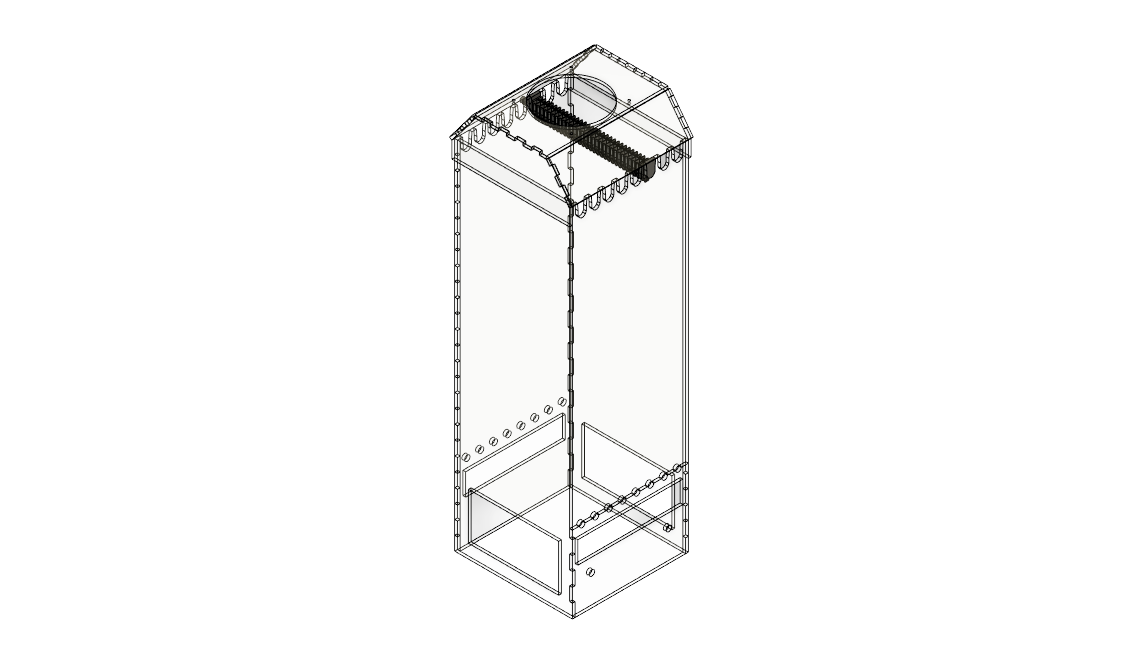
\includegraphics[scale = 0.4]{images/mywork/Sprint1/Column.png}
    \caption{The new DAC PMMA columns of ZEF}
    \label{fig:daccolumn}
\end{figure}

\begin{figure}[H]
\centering
\begin{minipage}{.5\textwidth}
  \centering
  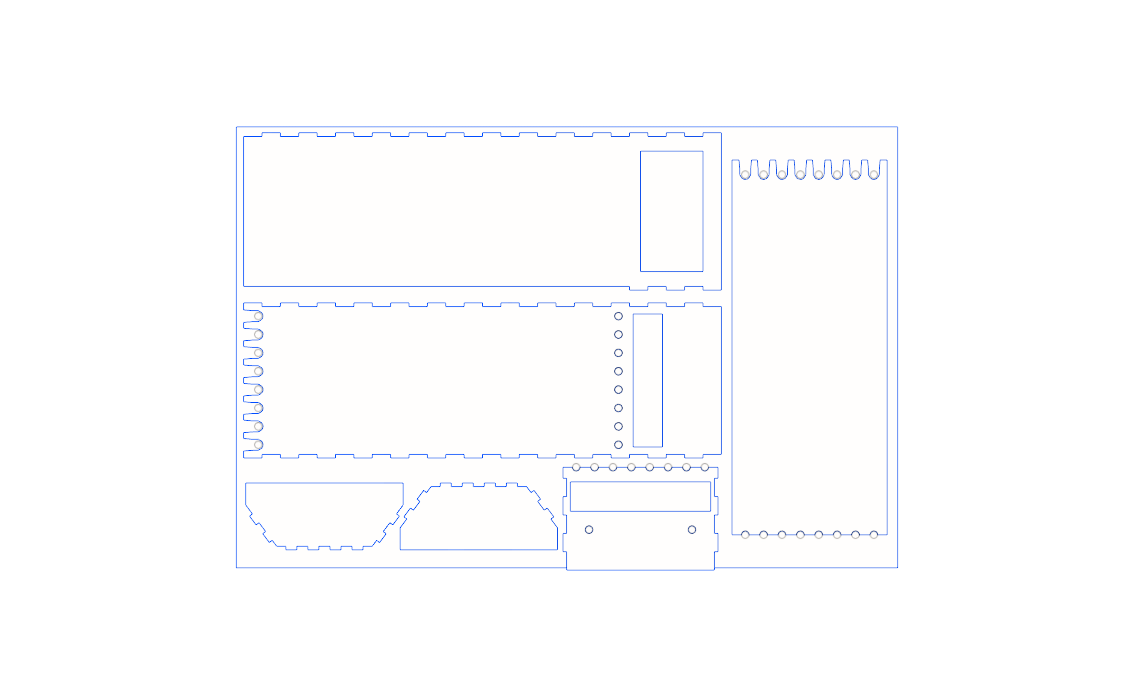
\includegraphics[width=\linewidth]{images/mywork/Sprint1/Lasersheet1.png}
  \captionof{figure}{PMMA sheet 1}
  \label{fig:pmma1}
\end{minipage}%
\begin{minipage}{.5\textwidth}
  \centering
  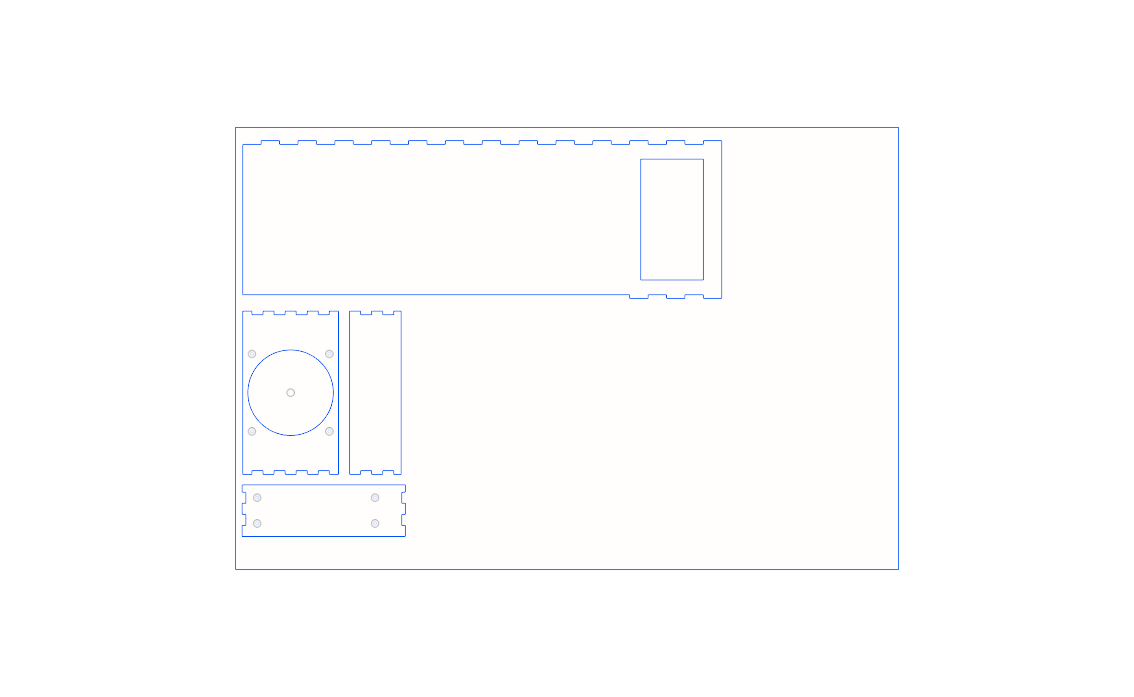
\includegraphics[width=\linewidth]{images/mywork/Sprint1/Lasersheet2.png}
  \captionof{figure}{PMMA sheet 2}
  \label{fig:pmma2}
\end{minipage}
\end{figure}

First, the DAC column which can be seen in full assembly in Figure \ref{fig:daccolumn} was fabricated using PMMA sheets which were purchased from Laserbeest. Based on the designs shown in Figure \ref{fig:daccolumn}, Jan had designed the PMMA sheets for the laser cutting for the assembly parts for the DAC column as well before my internship had begun. The PMMA sheet designs can be seen in Figure \ref{fig:pmma1} and Figure \ref{fig:pmma2}. The PMMA sheets were lasercut based on the above designs in the Industrial Department of TU Delft which took not more than 10 minutes. 
\bigbreak
The laser cut parts were then assembled in the ZEF workshop using duct tape as it still wasn't a final design. The PMMA cut parts fit perfectly with each other and can be seen in the Figure \ref{fig:pmmaass1} which contains the top hat for the fan that sucks air out of the DAC column to the atmosphere and Figure \ref{fig:pmmaass2} is the DAC column without the top hat, we can also see the DAC distributor fitting snuggly in the slots.  


\begin{figure}[H]
\centering
\begin{minipage}{.5\textwidth}
  \centering
  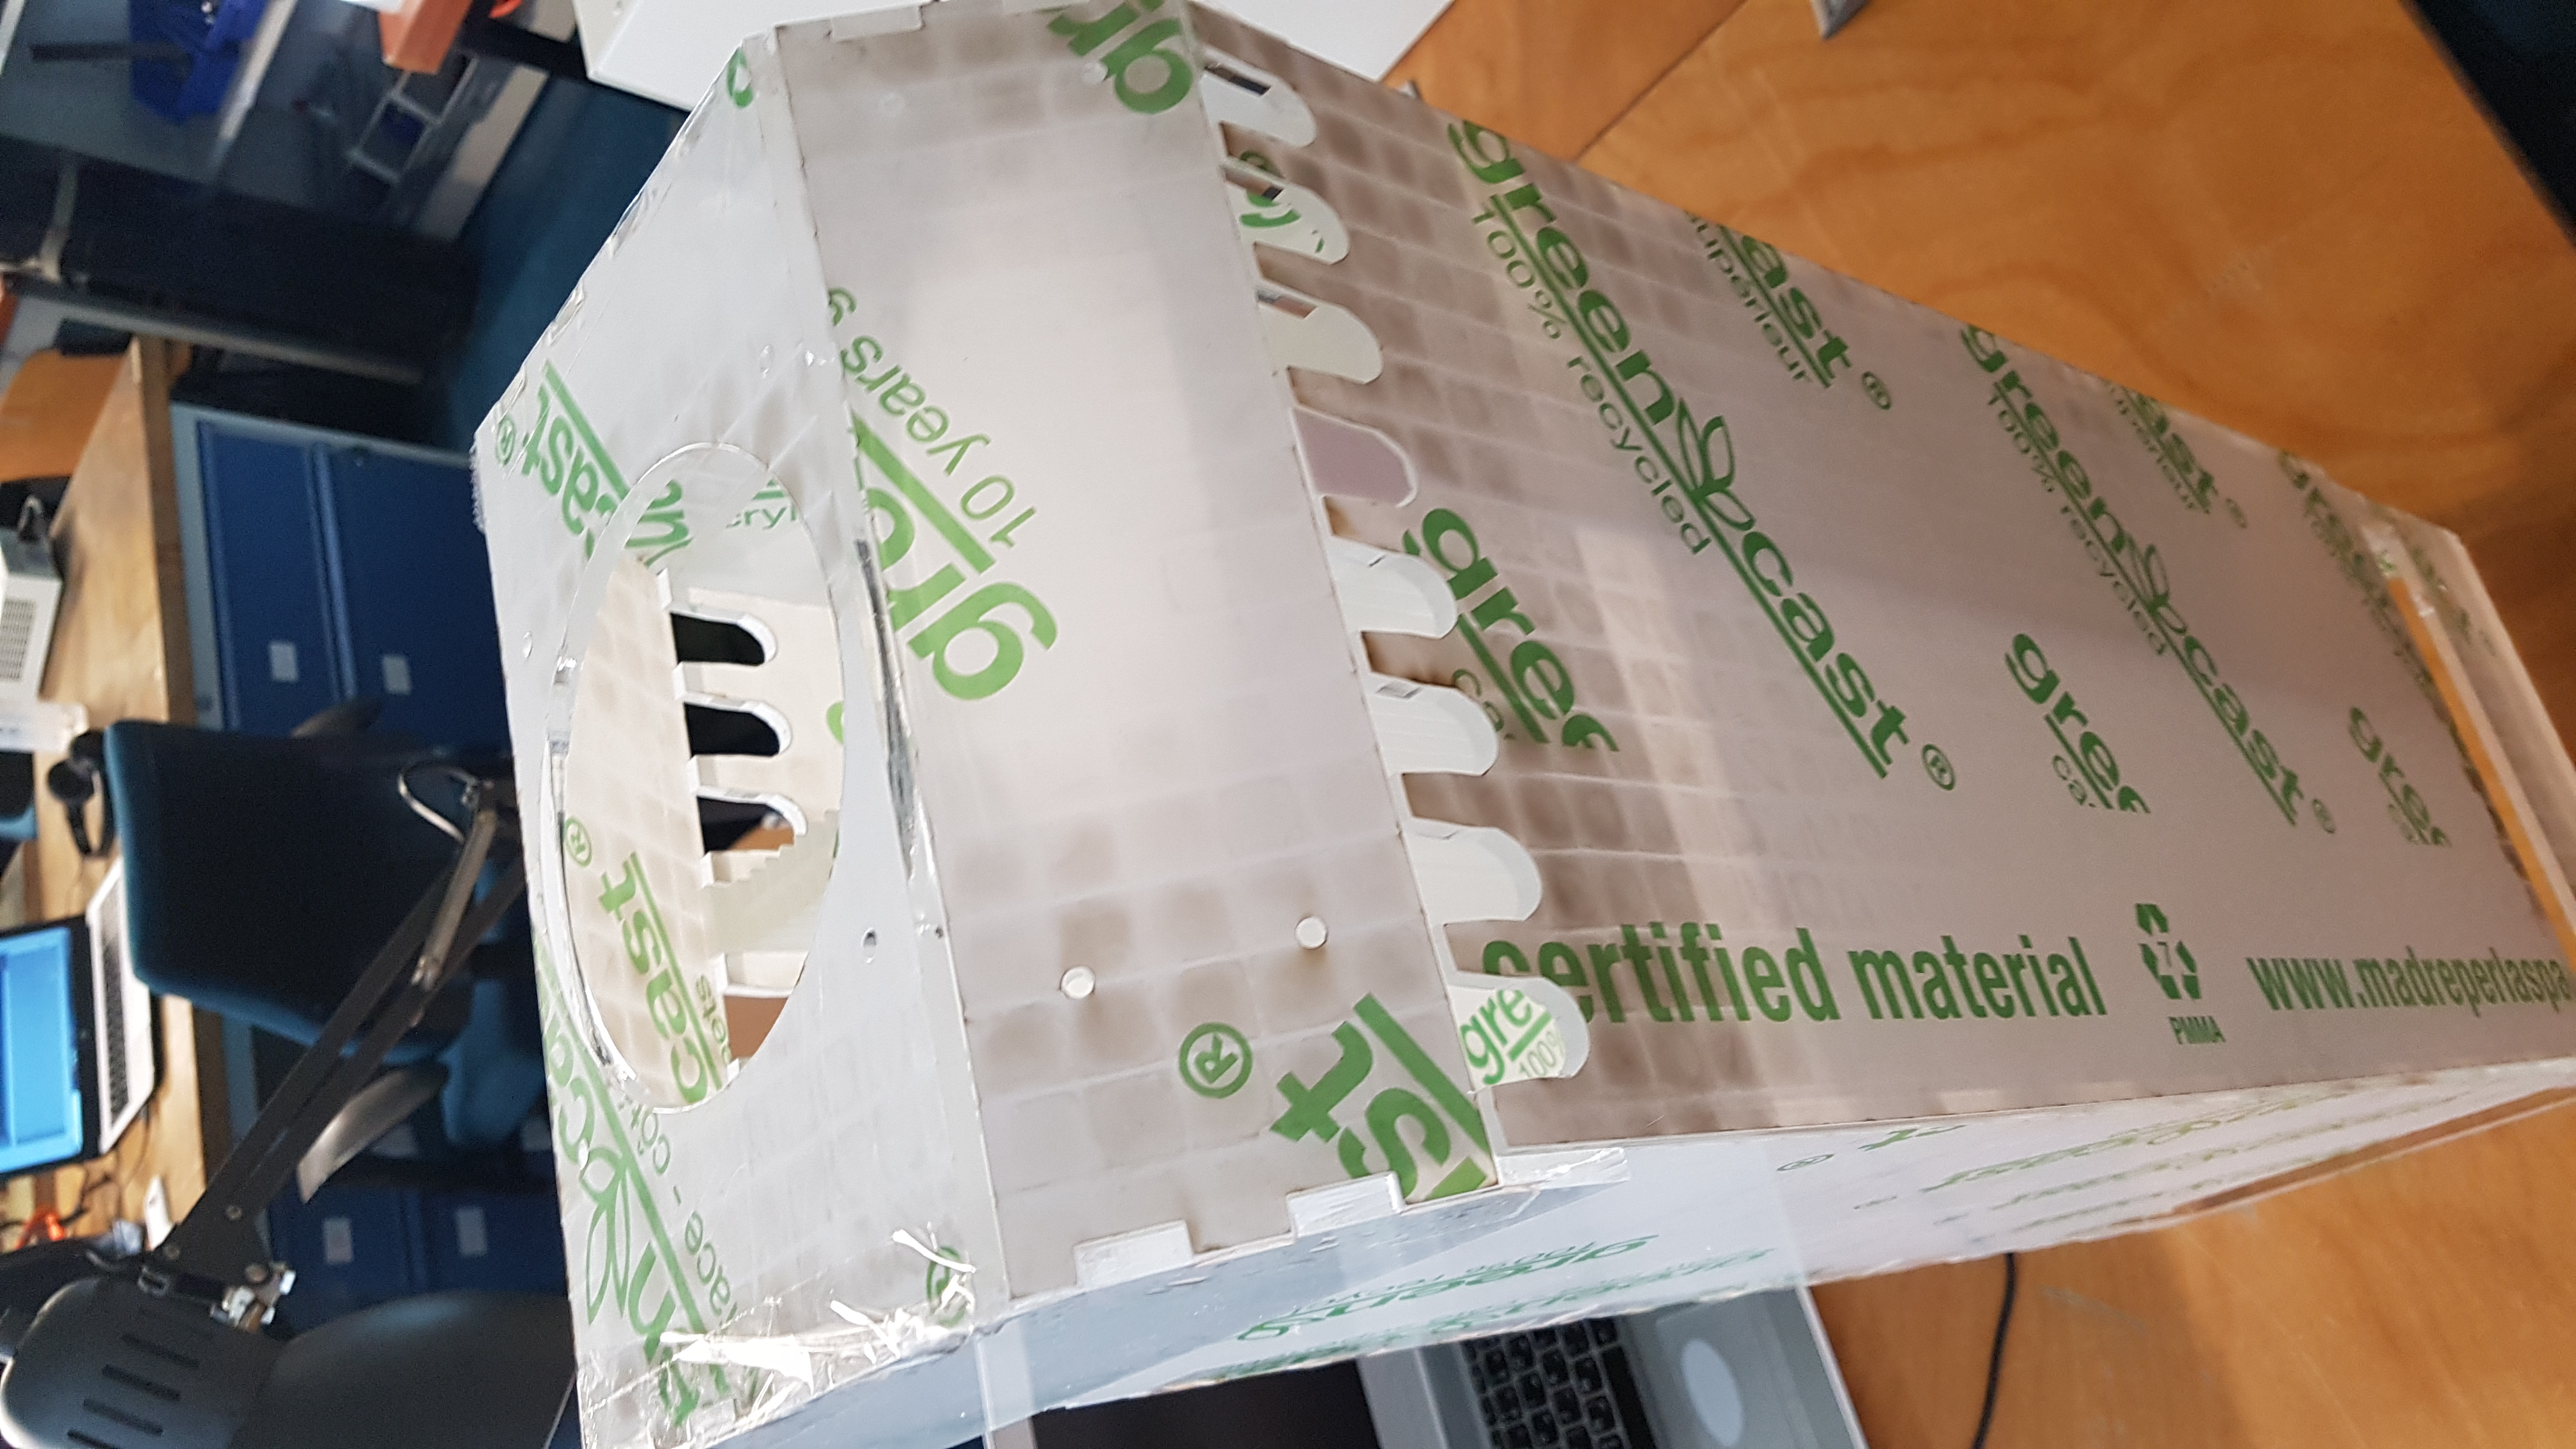
\includegraphics[width=\linewidth,angle = 270]{images/mywork/Sprint1/PMMAAssembled.jpg}
  \captionof{figure}{DAC column with top hat}
  \label{fig:pmmaass1}
\end{minipage}%
\begin{minipage}{.5\textwidth}
  \centering
  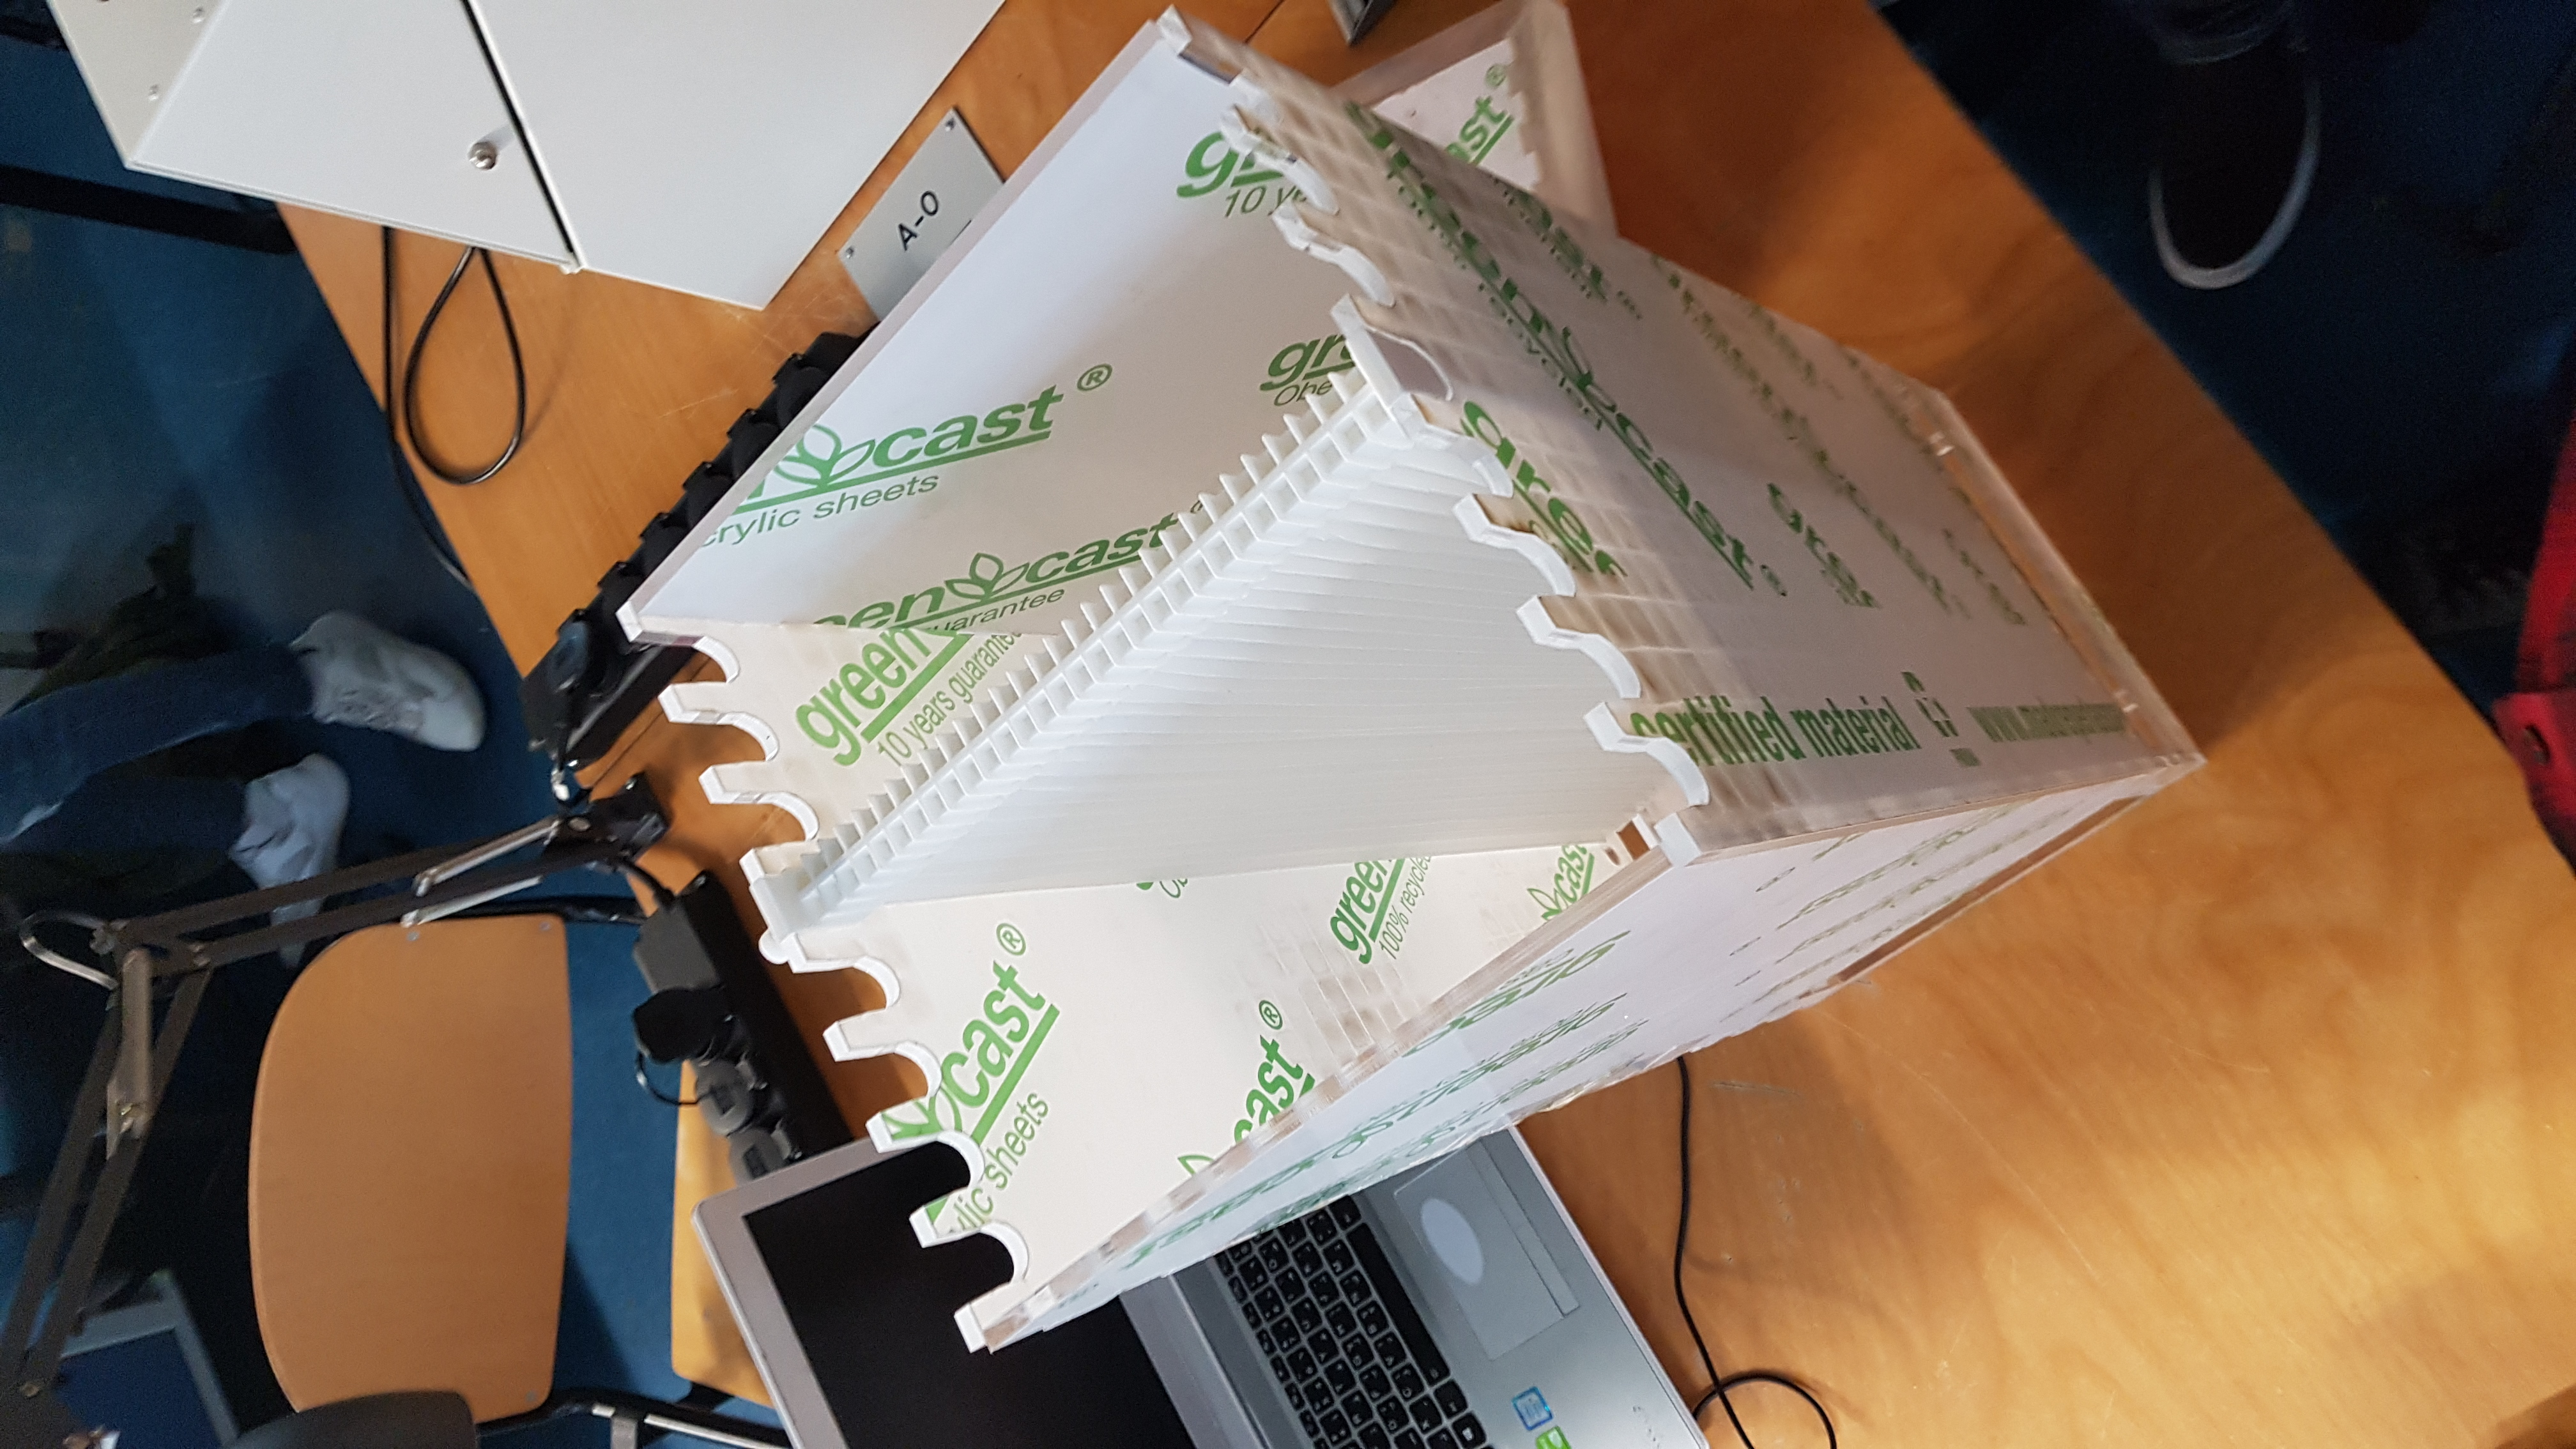
\includegraphics[width=\linewidth, angle = 270]{images/mywork/Sprint1/AssembledPMMA.jpg}
  \captionof{figure}{DAC column with distributor}
  \label{fig:pmmaass2}
\end{minipage}
\end{figure}

Based on ZEF IV designs for the distributor and manifold minor design changes were made inorder to make some parts more robust. The parts were manufactured using 3D printing with print material used as Polylactide (PLA). Since, the old DAC collectors had no design changes and weren't broken. We continued to use them with the new system as well, which were 3D printed by the previous team as well. The printer used was a Utimaker 2+ which was made with leaktight settings (high infill \% and very low layer height) in the Ultimaker Cura software for 3D printing. 

\begin{figure}[H]
\centering
\begin{minipage}{.5\textwidth}
  \centering
  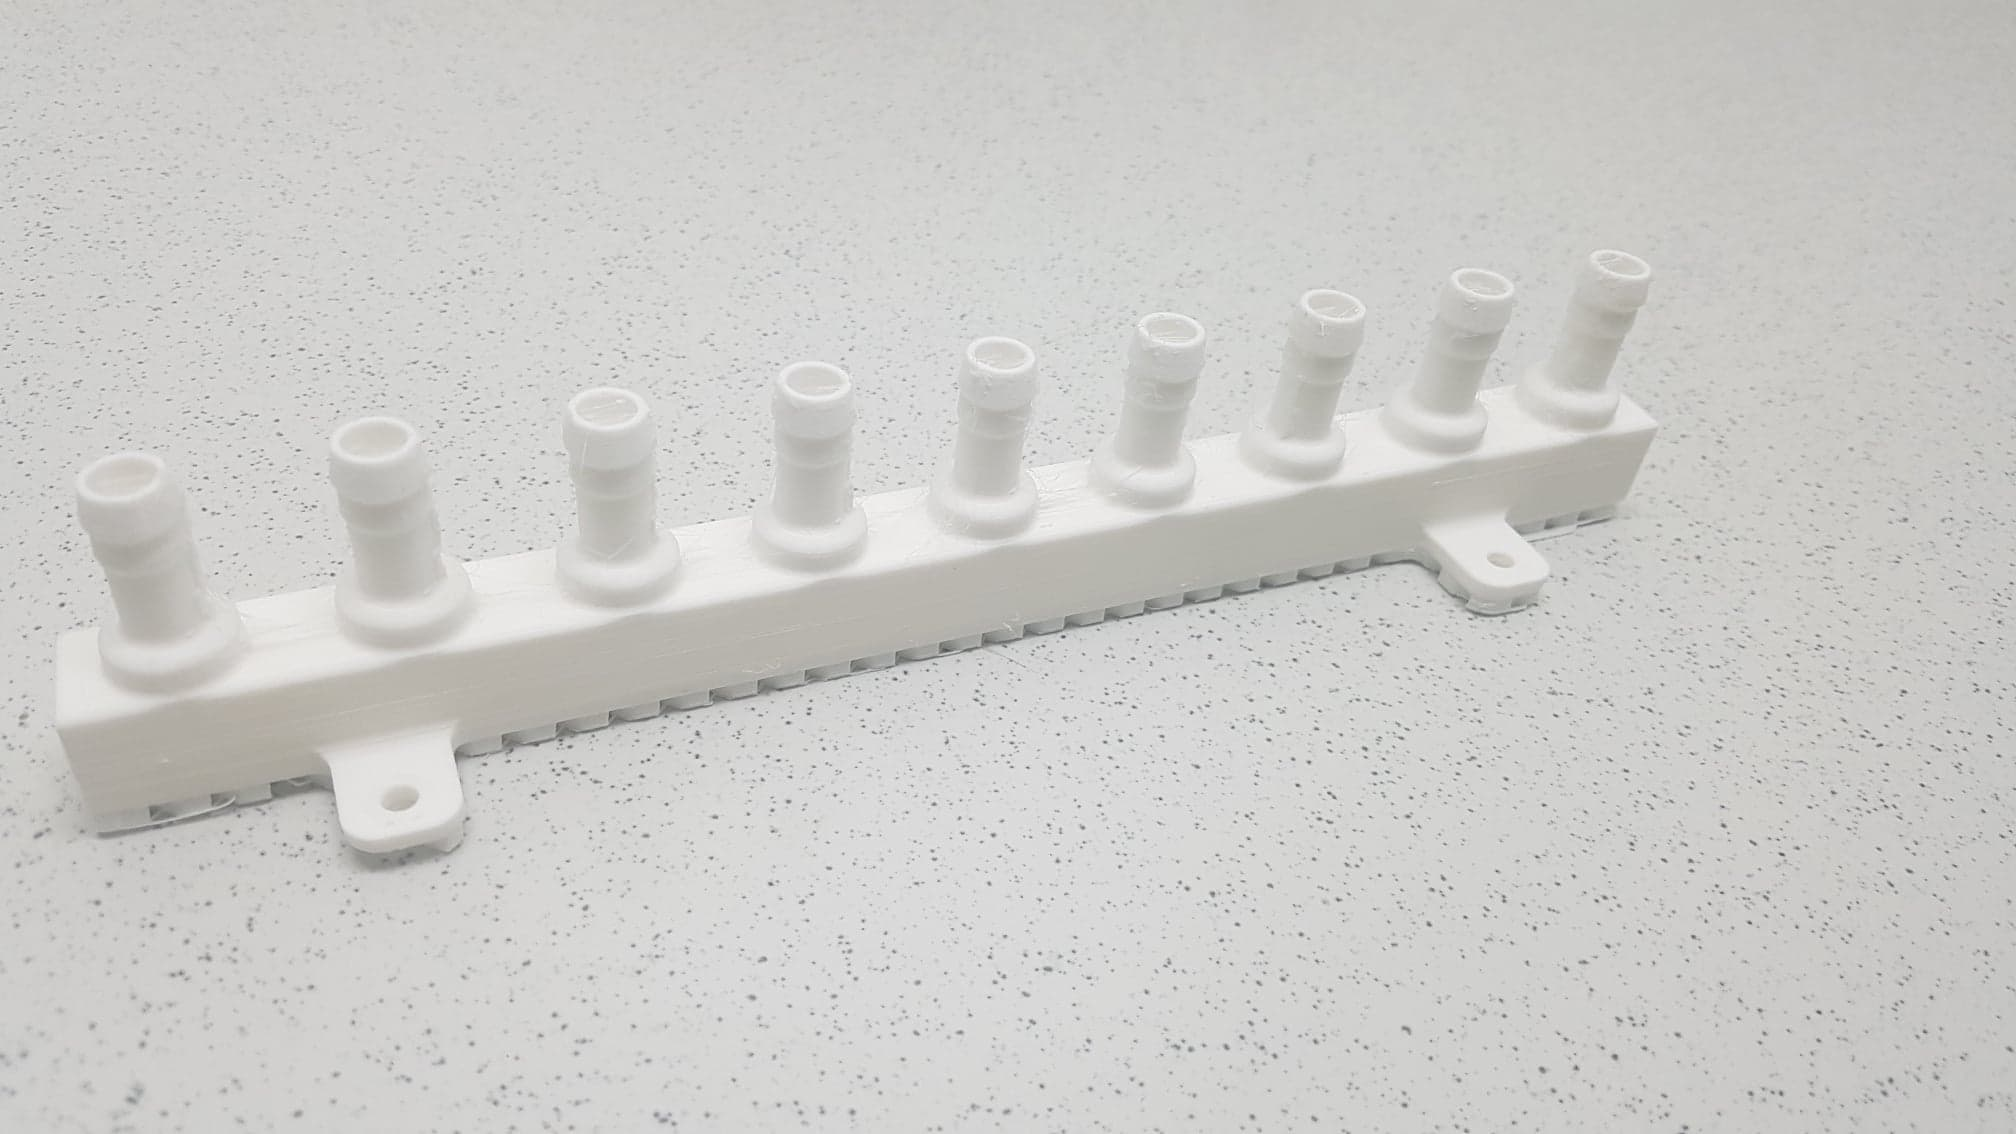
\includegraphics[width=0.9\linewidth]{images/mywork/Sprint1/Manifold.jpg}
  \captionof{figure}{3D DAC manifold}
  \label{fig:3Dmanifold}
\end{minipage}%
\begin{minipage}{.5\textwidth}
  \centering
  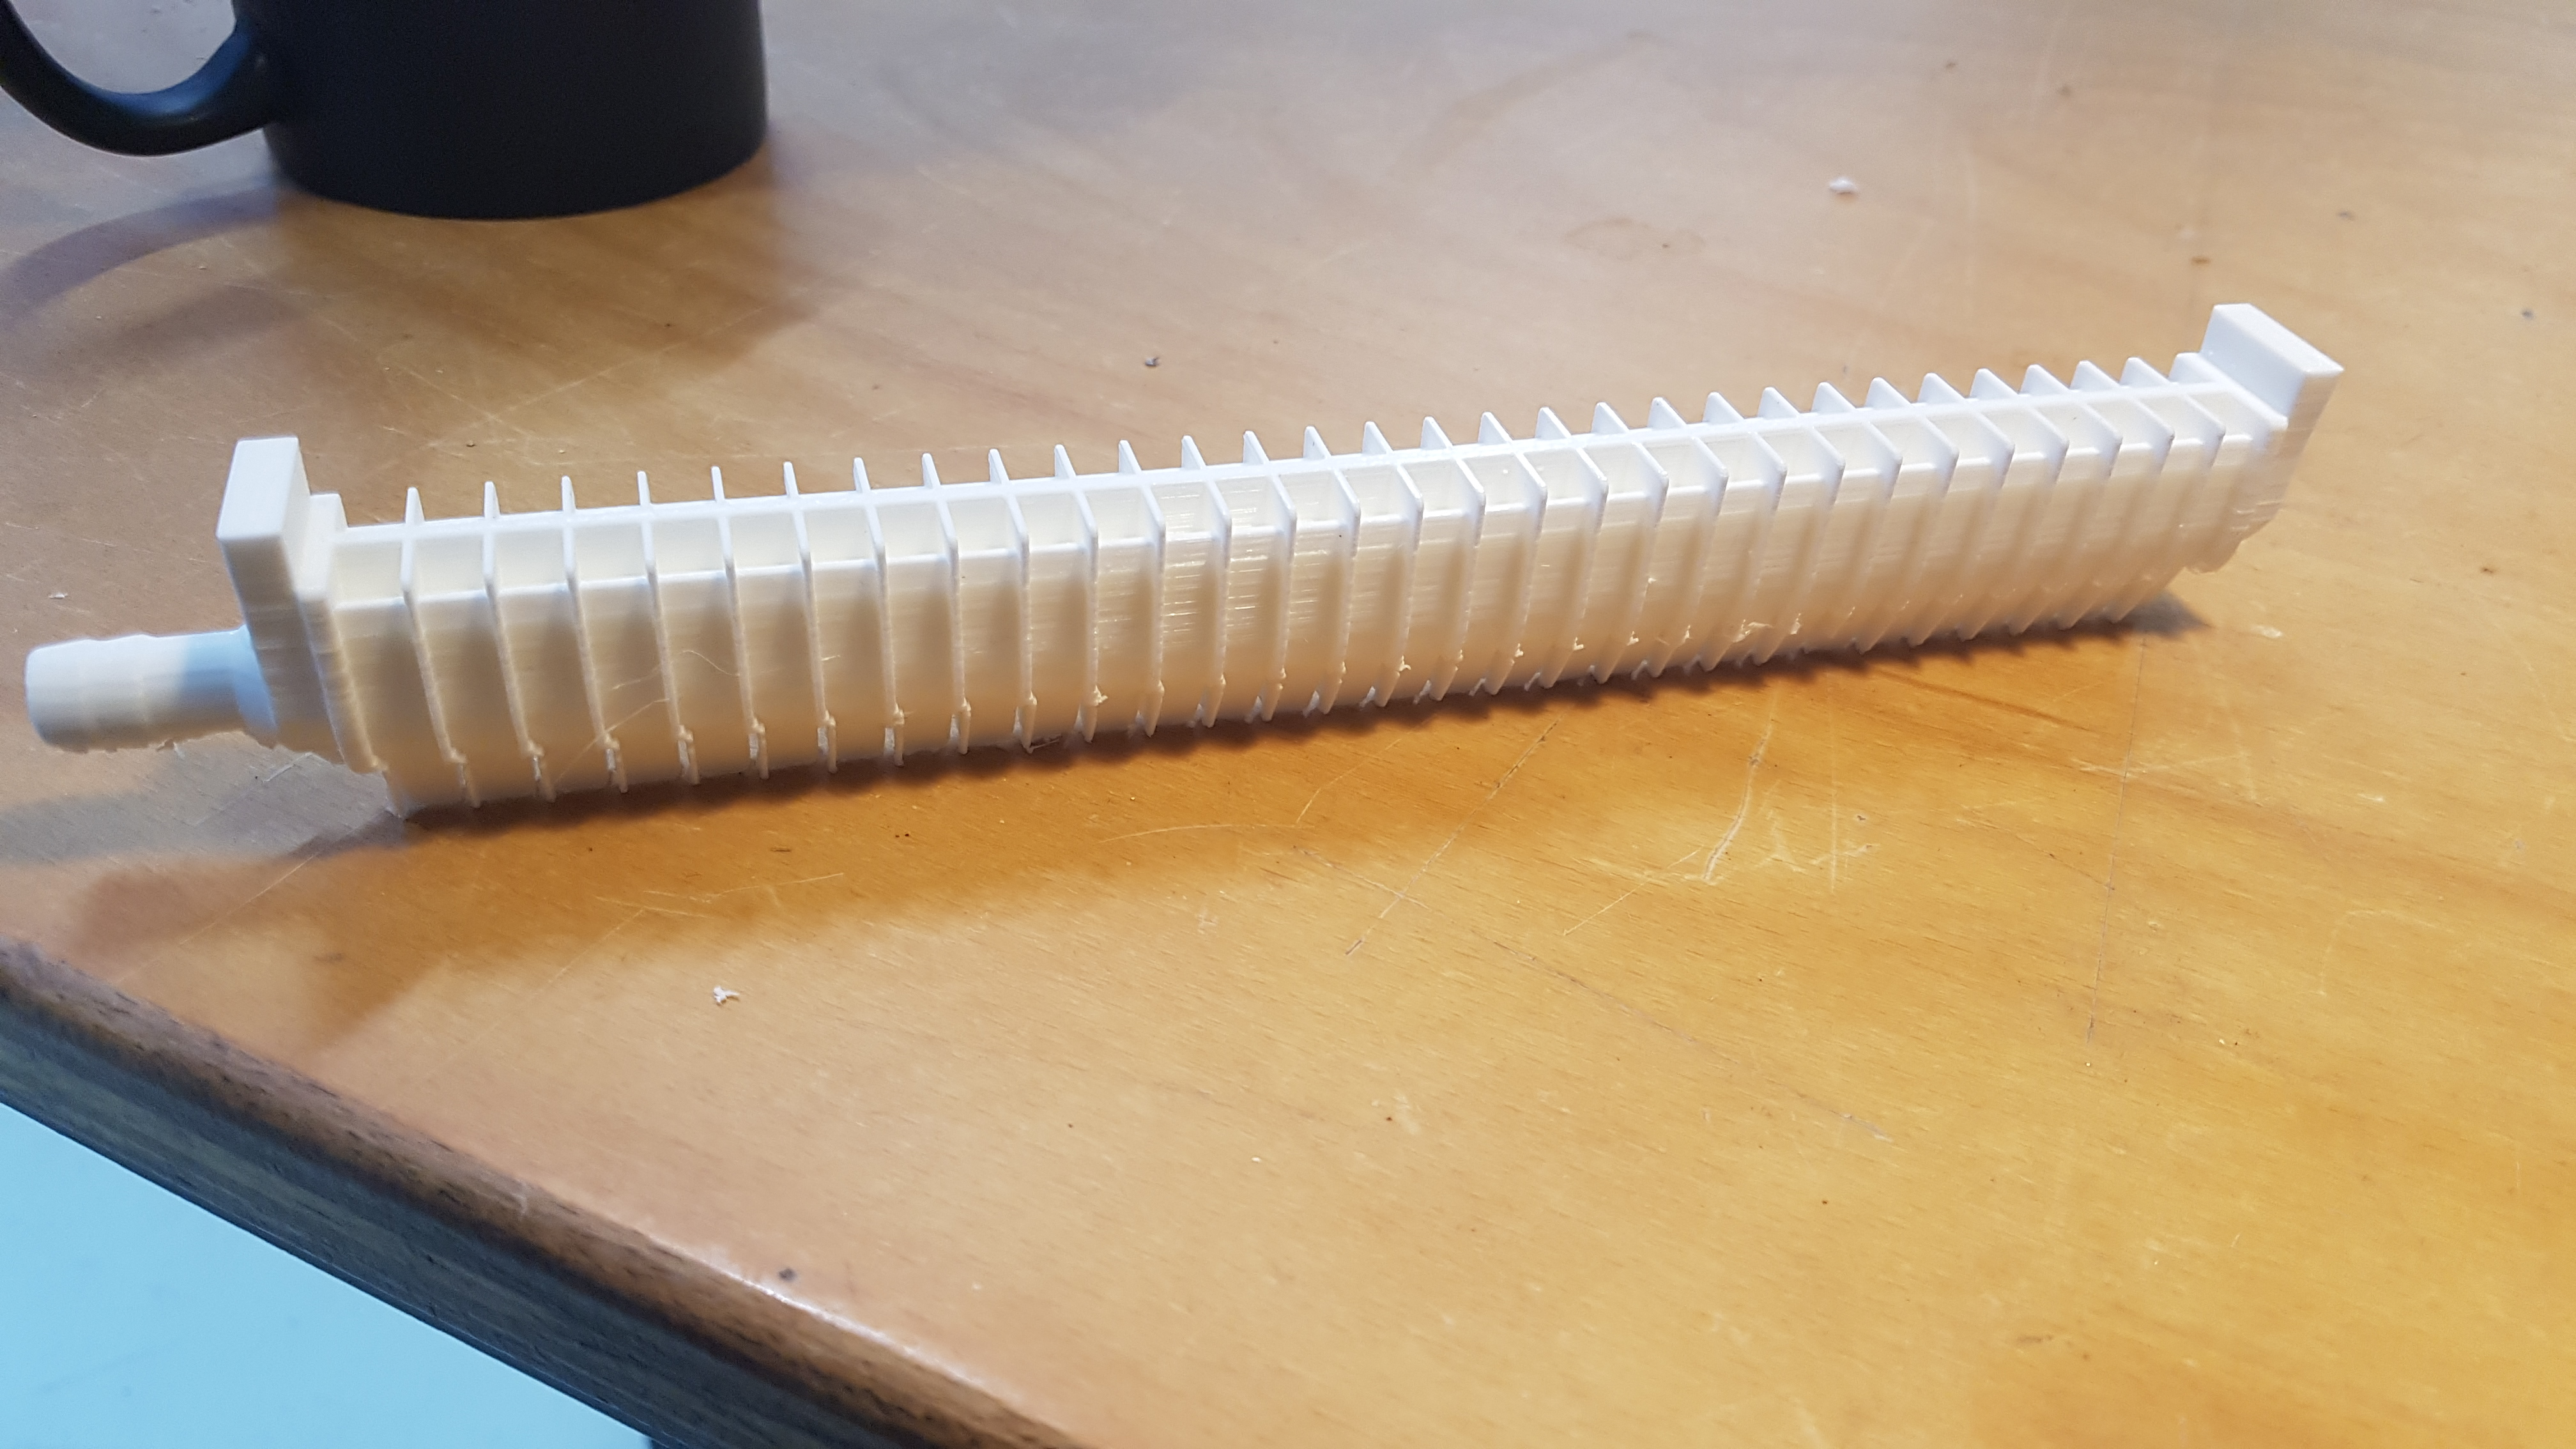
\includegraphics[width=0.9\linewidth]{images/mywork/Sprint1/Distributor.jpg}
  \captionof{figure}{3D DAC distributor}
  \label{fig:3Ddistributor}
\end{minipage}
\end{figure}

In Figures \ref{fig:3Dmanifold} we can see the final 3D printed DAC manifold and in Figure \ref{fig:3Ddistributor} we can see the final 3D printed distributor. It can be seen that in the Figure \ref{fig:pmmaass1} that there is a list of components needed for the DAC absorber column: 
\begin{itemize}
    \item DAC distributors x8 
    \item DAC manifold x1 
    \item DAC collectors X8 
    \item DAC flow channels x8
    \item DAC collector bucket x1 
    \item Silicon connecting pipes
\end{itemize}

Since, we needed a large number of DAC distributors and each 3D print take about 24 hours. We had to utilize the 3D printers at Industrial design department of TU Delft. For the DAC flow channels, we used the DAC system V1.0's flow channels itself and it had the same required specifications. The channels were ordered from an external company called Windowprint. The channel is cut across its width and halved. It is then cut to the required shape and stuck to each other using a plastic sealing machine (mostly used to seal sandwich bags). Finally, they are fitted into the DAC distributor and placed inside the DAC absorber column with the DAC collectors. The final assembly of the DAC absorber column can be seen in Figure \ref{fig:absorber} below.  

\begin{figure}[H]
    \centering
    \includegraphics[scale = 0.155]{images/mywork/Sprint1/absorber.png}
    \caption{Complete DAC absorber column}
    \label{fig:absorber}
\end{figure}

\subsection{Sprint 2 - $23^{rd}$ September to $14^{th}$ October}

During the sprint 2 period of my internship spanning from $23^{rd}$ September to $14^{th}$ October. I turned my attention toward the desorbtion part and running the DAC system V1.1 as one whole unit and getting the pumps and compressor to run using an Arduino 2560MEGA.  

\subsubsection{DAC system V1.1 desorber}
\label{sec:faultycomp}

The desorber unit which consists of a desorbtion chamber that heats the PEI to a set temperature (normally set to 80 \degree C) which can be controlled using temperature sensors and arduino code. The PID heater controller arduino code can be further examined in Appendix \ref{ap:arduino}. In the previous Section \ref{sec:zef4}, we have seen that they have already fabricated and used the desorbtion chamber and a vacuum pump to suck the absorbed $CO_2$ from the heated PEI in the desorbtion chamber using Pressure swing desorbtion. The desorber unit also consists of the PEI pump which was inoperational due to lose connections and incorrect code. The motor is now operational with proper connections in the bread board and with the the new "Motor starting" arduino code which starts the servo motor and sets the RPM of the motor as well, refer Appendix \ref{ap:arduino} for further examination. %refer picture in the zef4 section and explain about it

\begin{figure}[H]
\centering
\begin{minipage}{.5\textwidth}
  \centering
  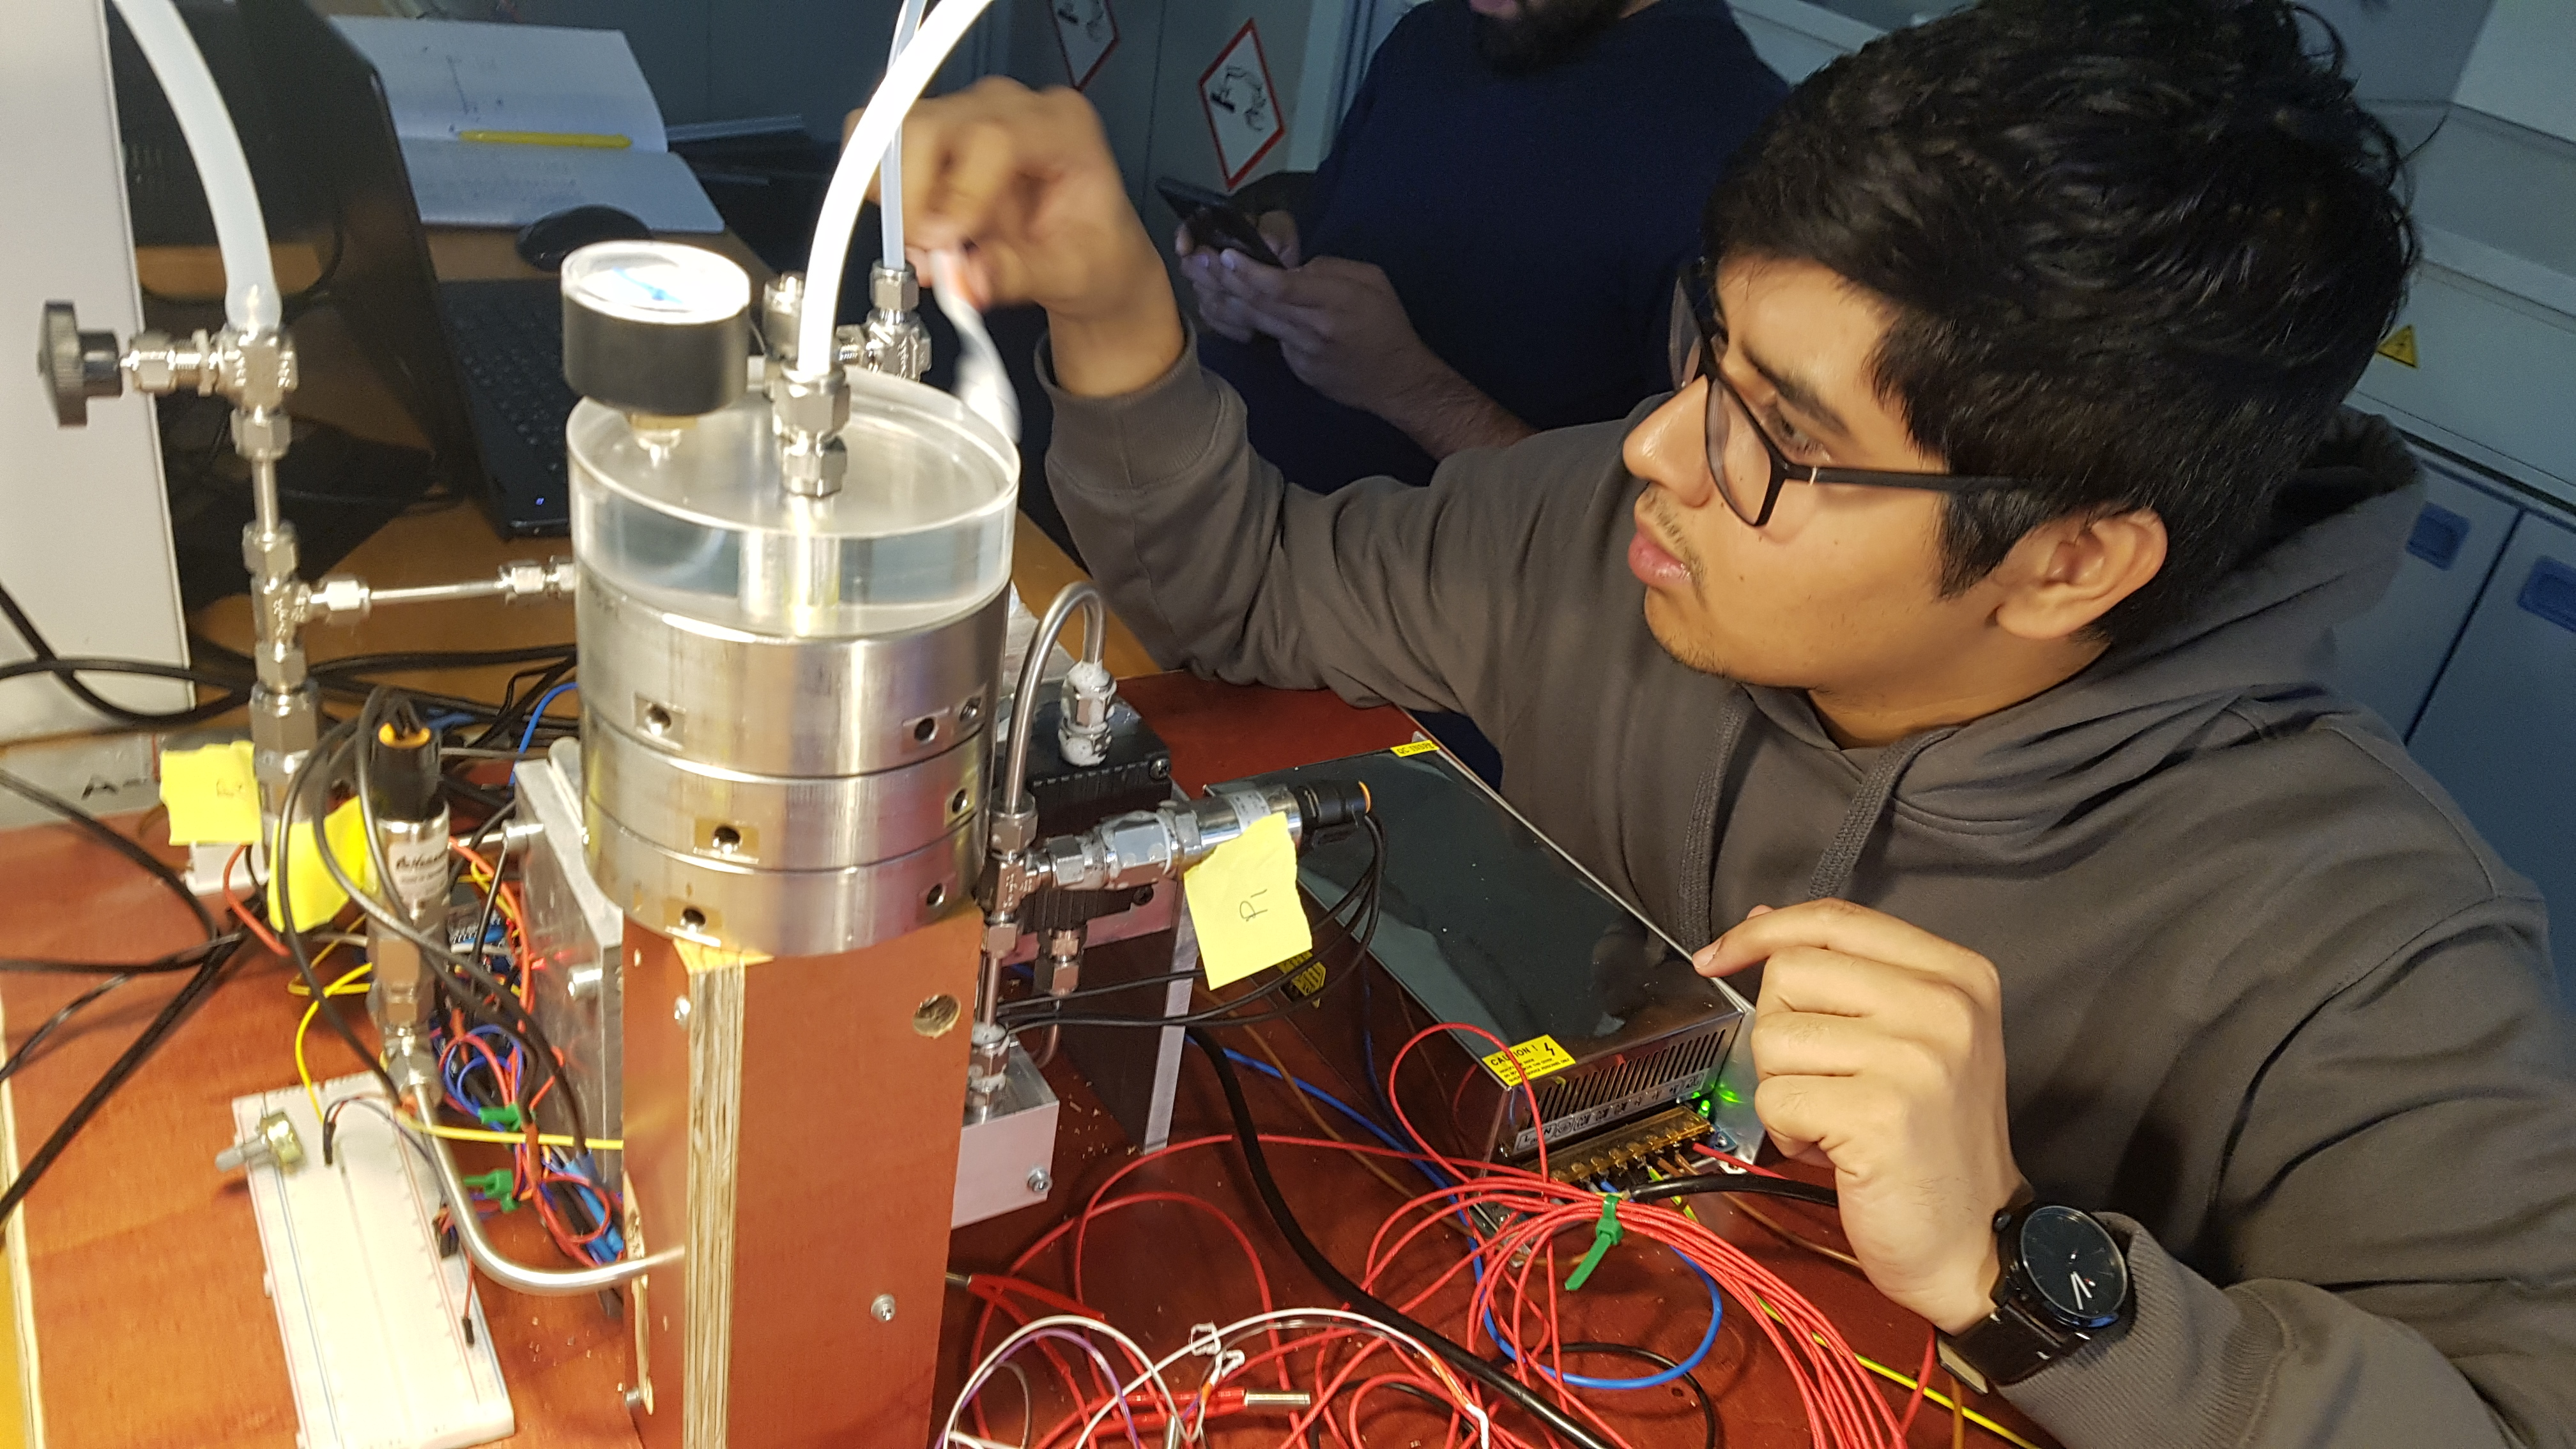
\includegraphics[width=0.9\linewidth]{images/mywork/Sprint2/Leaktest.jpg}
  \captionof{figure}{Leak test with bubbles}
  \label{fig:leaktest}
\end{minipage}%
\begin{minipage}{.5\textwidth}
  \centering
  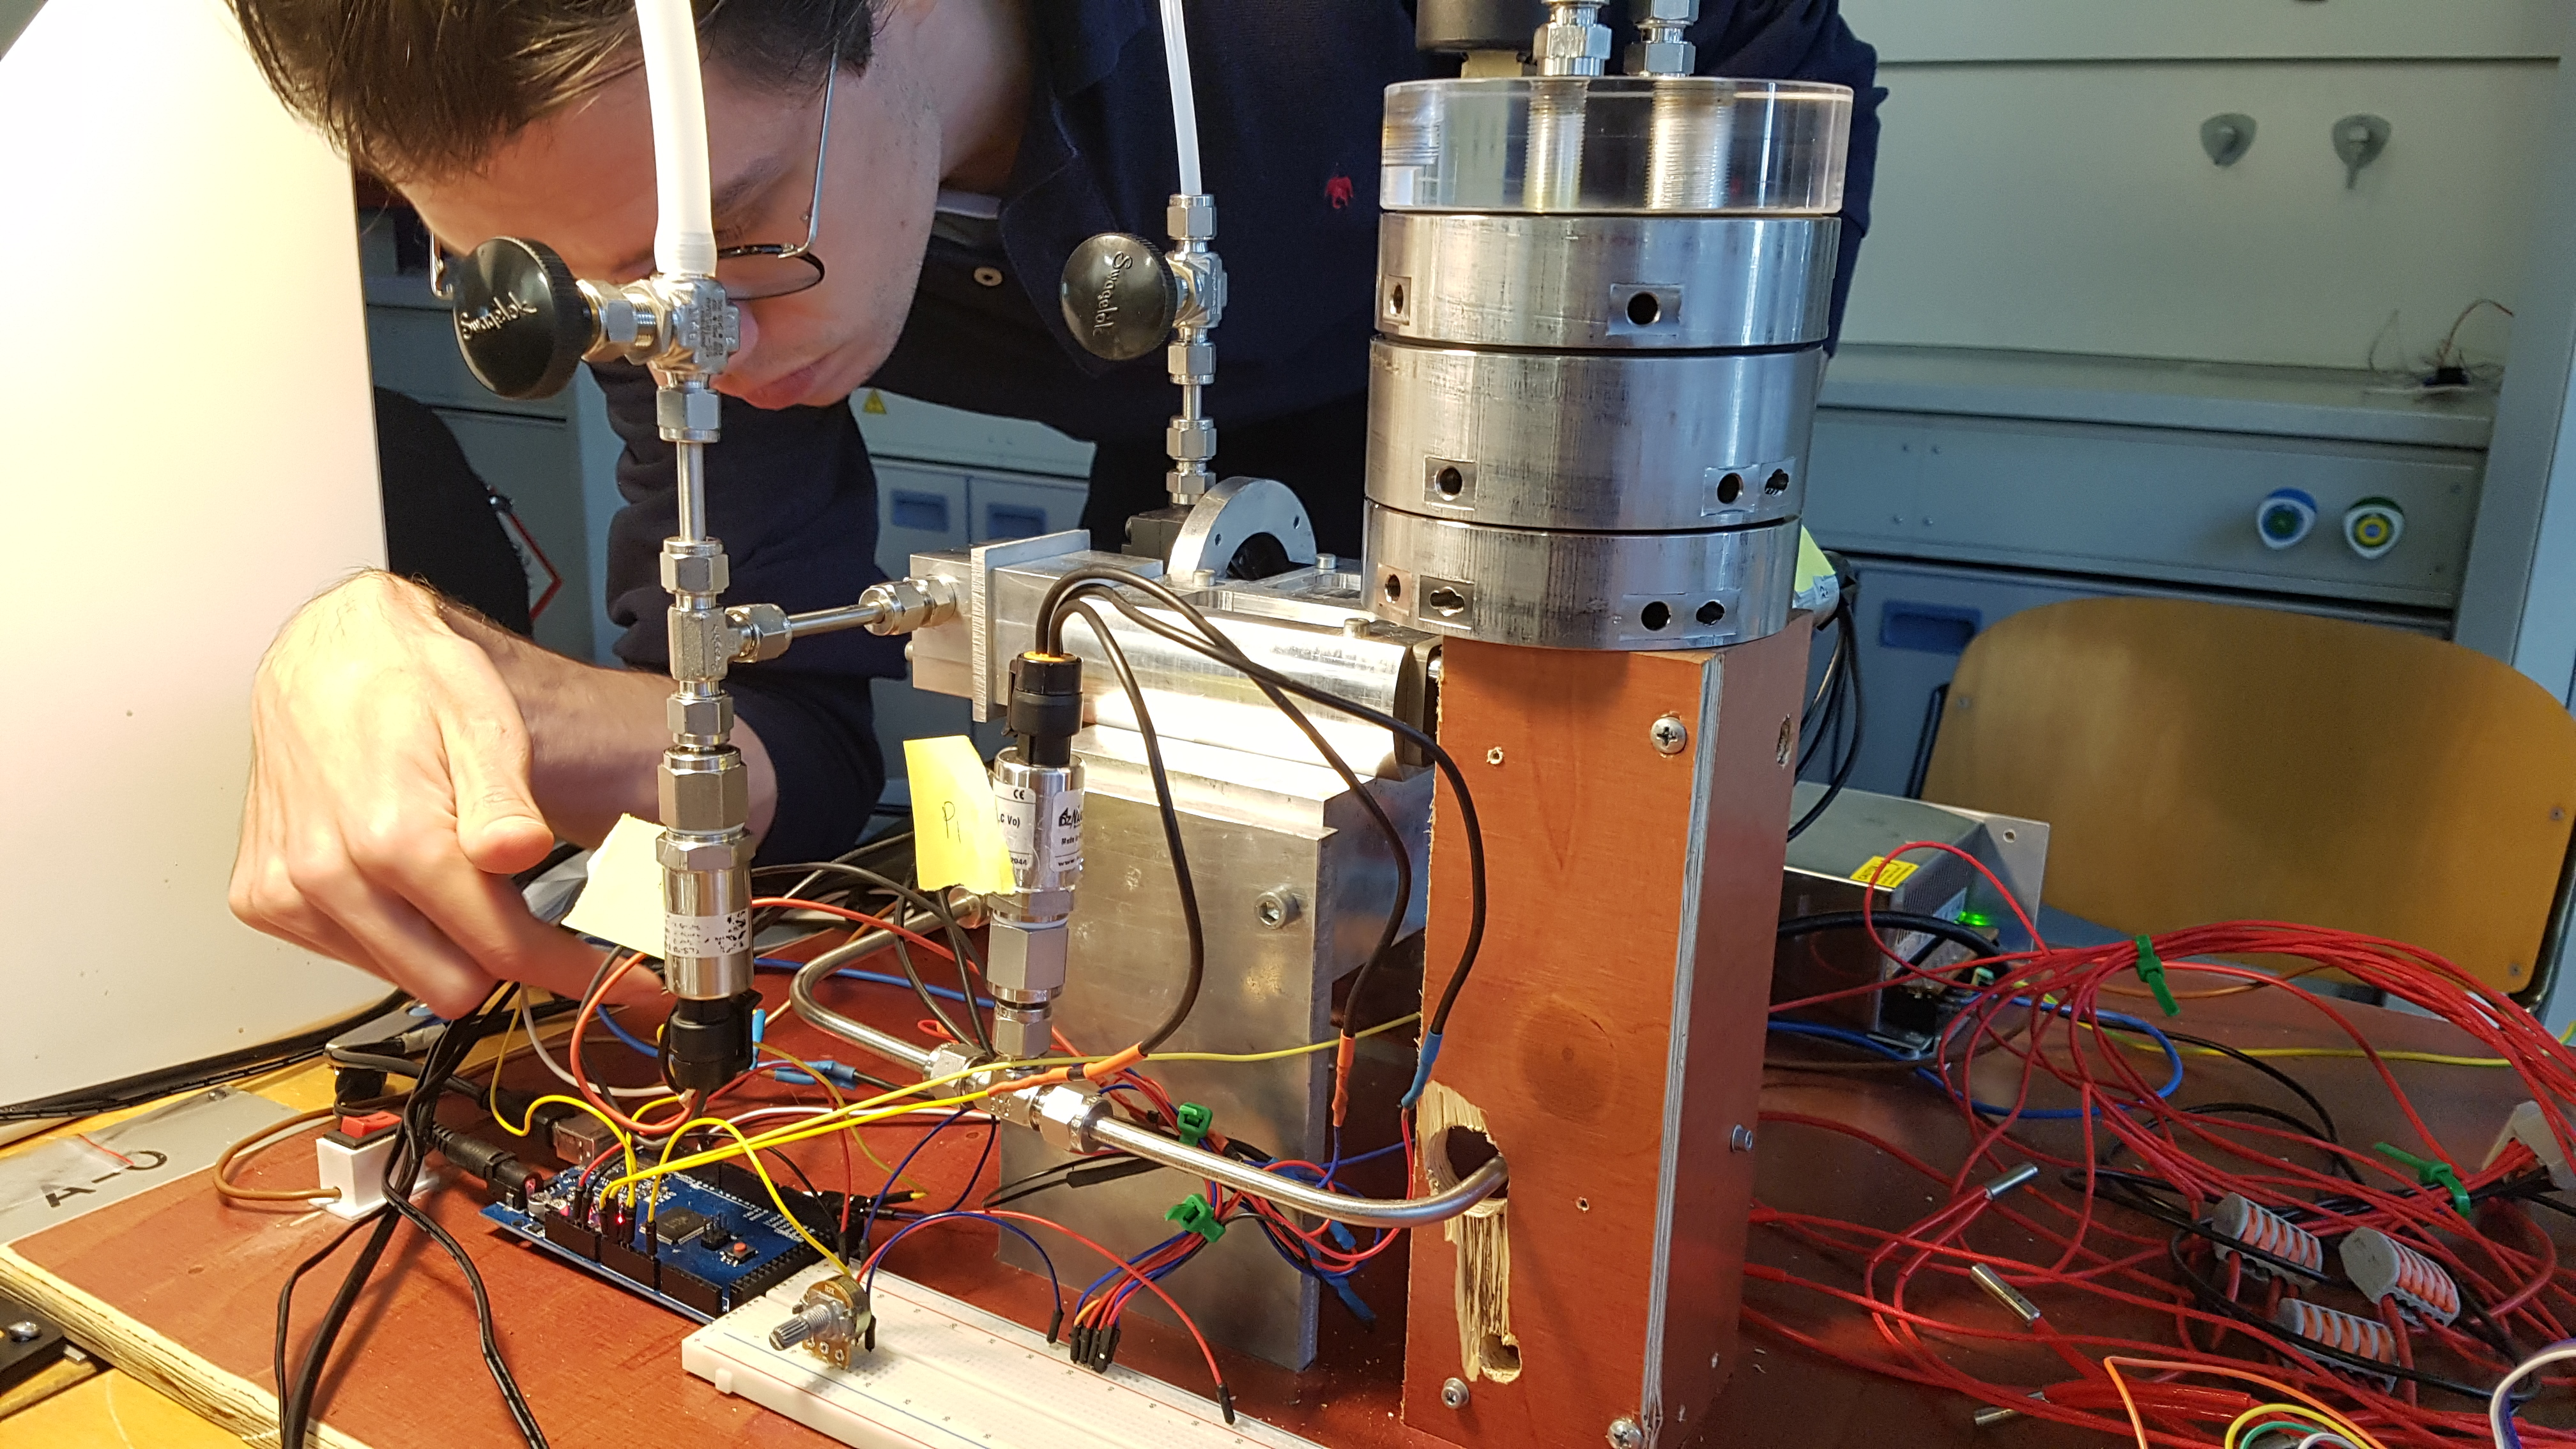
\includegraphics[width=0.9\linewidth]{images/mywork/Sprint2/desorbcheck.jpg}
  \captionof{figure}{Pressure sensor check}
  \label{fig:desorber}
\end{minipage}
\end{figure}

\begin{figure}[H]
    \centering
    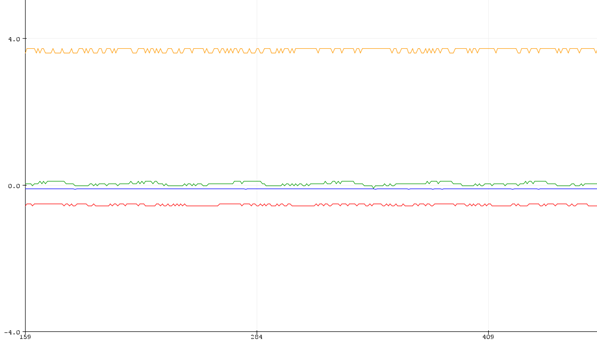
\includegraphics{images/mywork/Sprint2/pressuresensor.png}
    \caption{Pressure sensor outputs : Blue - P1, Red - P2, Green - P3 and Yellow - P4}
    \label{fig:psensor}
\end{figure}


The DAC system V1.1 desorber can be seen in Figure \ref{fig:desorber}. Since the desorber components were already present. I conducted leak tests and running the system for sometime to see if there is any issue with the PEI pump or the vacuum compressor. A point to note is that the system was designed to produce 50 bar pressure but on running it is found that the $3^{rd}$ stage of the compressor isn't pumping at the designed pressure ratio. This can be seen in the Figure \ref{fig:psensor} where the maxmium pressure output from the 4 stage compressor system is only below 4 bar pressure. It can also be seen that the P1,P2 and P3 are all around 0 bar pressure line which is not at all a desired output.
\bigbreak 
It was concluded to be due to leaks being present in the compressor system. So, leak tests were conducted as seen in Figure \ref{fig:leaktest} to see if there were any bubbles moving due to leaked gases at the Swagelok joints of the compressor system but the compressor had passed the leak test. On further examination by Pim (the LIS student who built the system), he pointed out that one of the Swagelok joints were in inch standards and not in the metric standards that we were using throughout the the system. 

\begin{figure}[H]
    \centering
    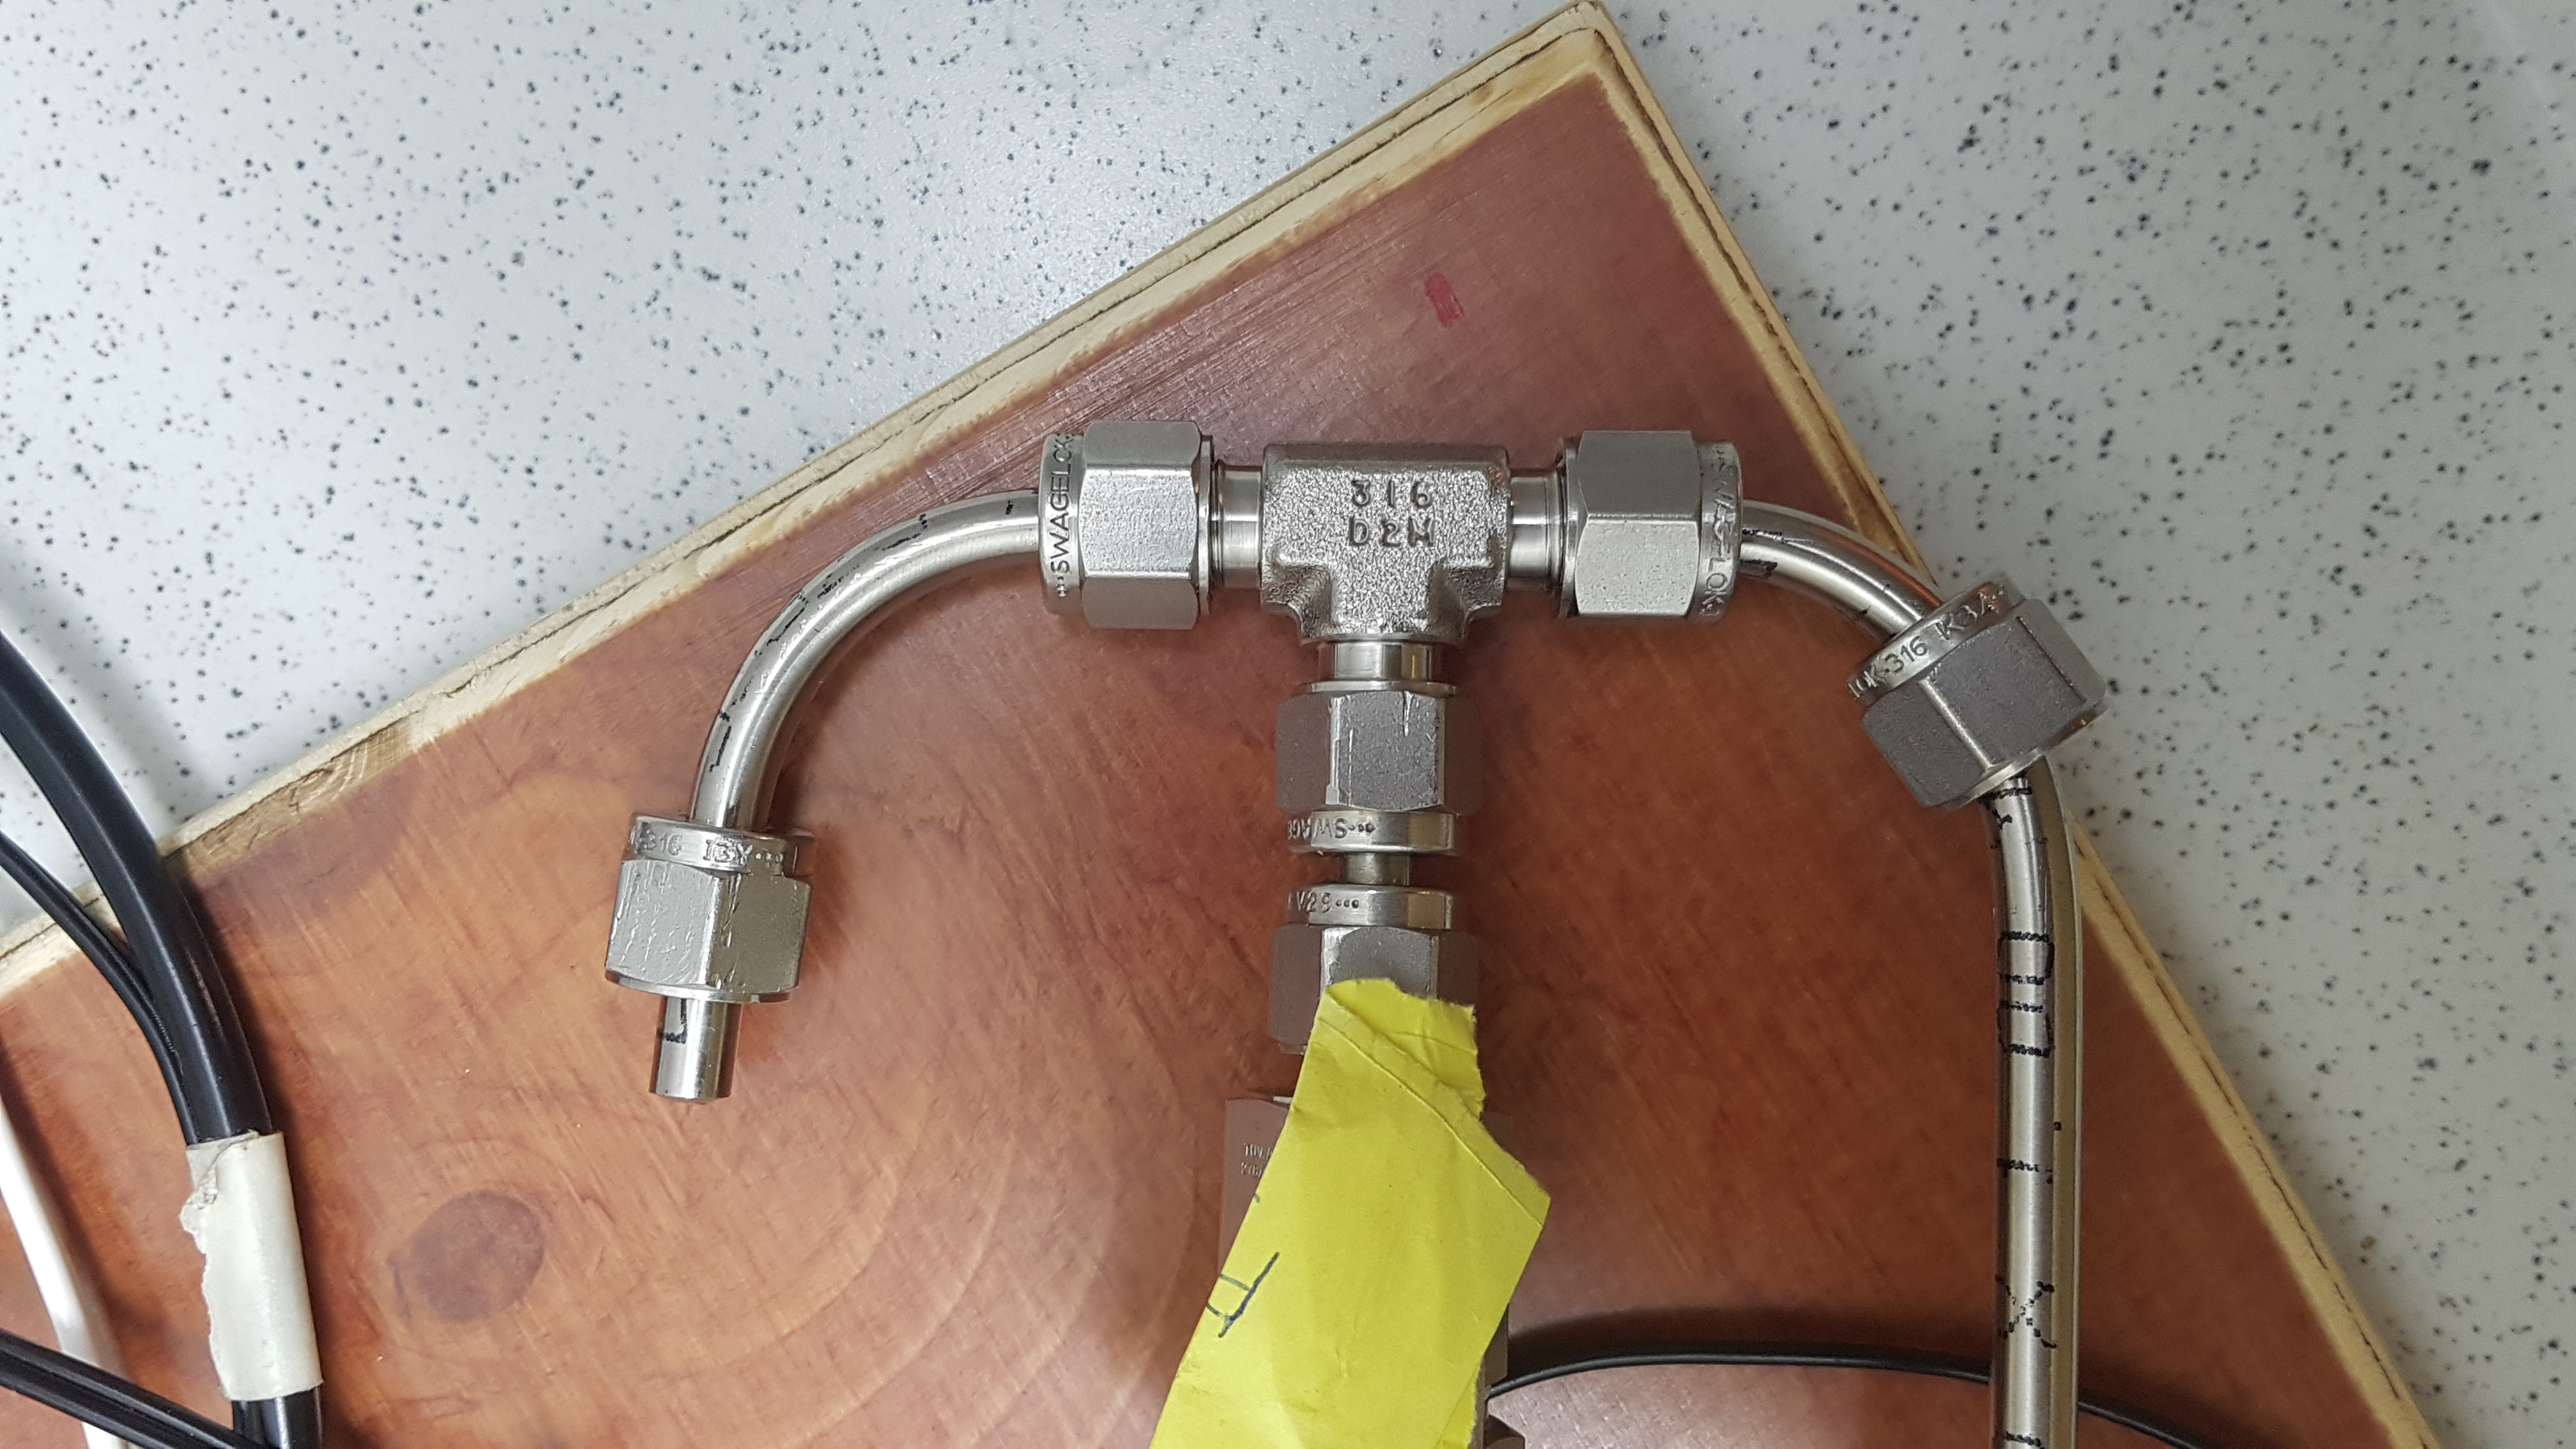
\includegraphics[scale = 0.07]{images/mywork/Sprint2/swagelok.jpg}
    \caption{Fixed the Swagelok joint}
    \label{fig:swagiss}
\end{figure}

In Figure \ref{fig:swagiss} the metric swagelok nuts are indicated by the small ring like feature below the octagonal feature used to hold the spanner. As seen in the figure, all the joints are fixed and made with metric bolts as per Pim's suggestion. Finally, the DAC system is complete and system is made to run. 

\subsubsection{Running DAC system V1.1}

During the second half of the sprint, once the absorber and desorber subsystems of the DAC system V1.1 is complete. The system components were connected together using silicon connecting pipes so that PEI can flow through the system. The fluid will be fed into the system using the collector bucket and then fluid shall be pumped across the system using the PEI pump. 
\bigbreak
First, in order to ensure that there is no leaks in the system. Water was passed through the system - which was quite a bad idea since some of the water went into the vacuum compressor system. However, it turned out to be fine as all the water was cleared out. Once the water was all cleared out, PEI was passed into the system and made to run in the system and the system is closed. A proper flow of PEI was occurring with minimal to no leaks or spills. However, all the wiring was in a haphazard manner and I was told to make the electronic circuits into modules. Which was done using transparent boxes from Gamma store. Holes were created in the boxes so that wires can go from inside the box to outside the box and vice versa.
\bigbreak 
In Figure \ref{fig:dacsystem1.1}, we can see the complete DAC System V1.1 with all the components working together as one unit. In the background you can see the old broken down DAC System V1.0 of ZEF IV team. The following are the labelled components of the DAC system: 

\begin{itemize}
    \item 1 - DAC Absorber V1.1 
    \item 2 - DAC Desorber V1.1 
\end{itemize}

\begin{figure}[H]
    \centering
    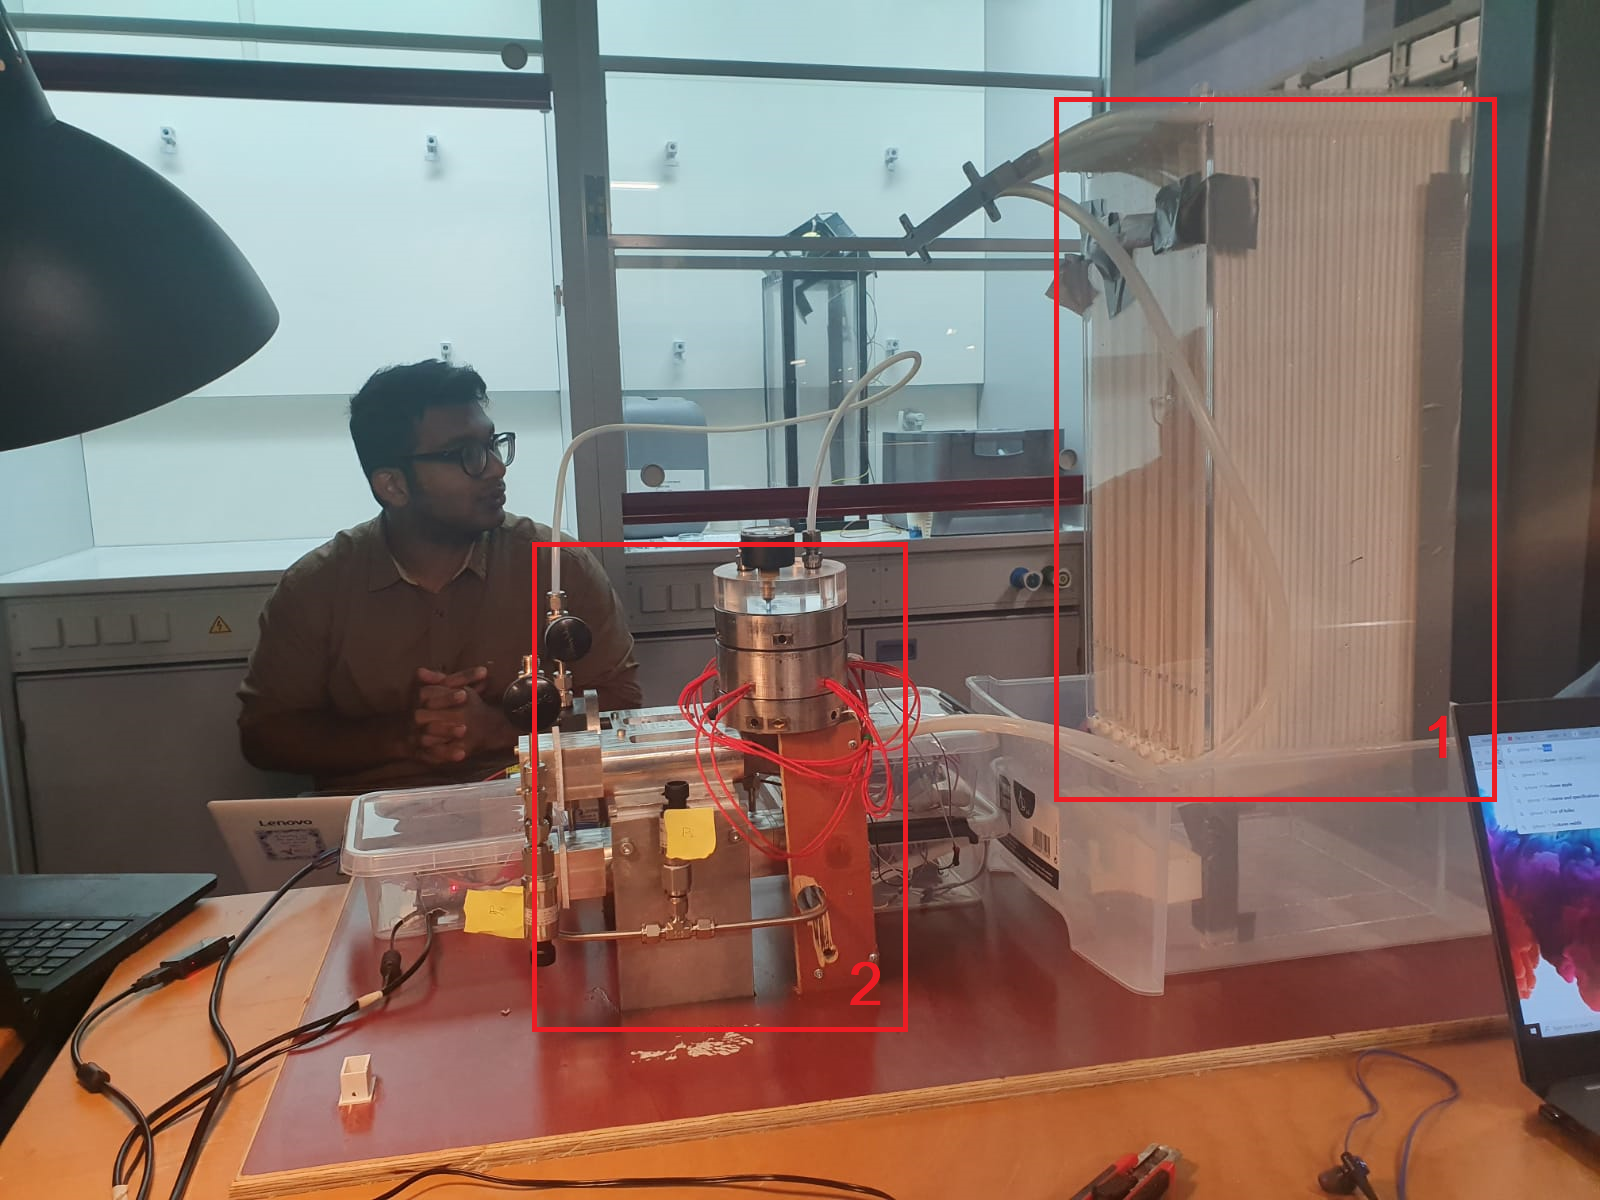
\includegraphics[scale = 0.45]{images/mywork/Sprint2/dacsystem1.png}
    \caption{The complete DAC System V1.1 }
    \label{fig:dacsystem1.1}
\end{figure}


\subsection{Sprint 3 - $14^{th}$ October to $4^{th}$ November}

Sprint 3 proved to be one of the toughest parts of the internship since it involved a lot of messy work since we were working with PEI and heartbreak since mid-sprint our system broken down. The reasons for the system breakdown shall be elaborated more in the Section \ref{sec:breakdown}. On running the system continuously for hours, we could make some quite interesting observations which can be seen in Section \ref{sec:obs}.  

\subsubsection{Running the DAC System V1.1 for long times with PEI}
\label{sec:obs}

We ran the DAC System V1.1 for about 7.23 hours cumulatively at varying RPMs of the PEI pump motor for various test conditions before the system broke. At first, we loaded PEI into the system from the desorbtion chamber without heating the desorbtion chamber. It can be seen in the Figure \ref{fig:peiloading}. This was done just to observe how PEI is flowing through the system. 

\begin{figure}[H]
    \centering
    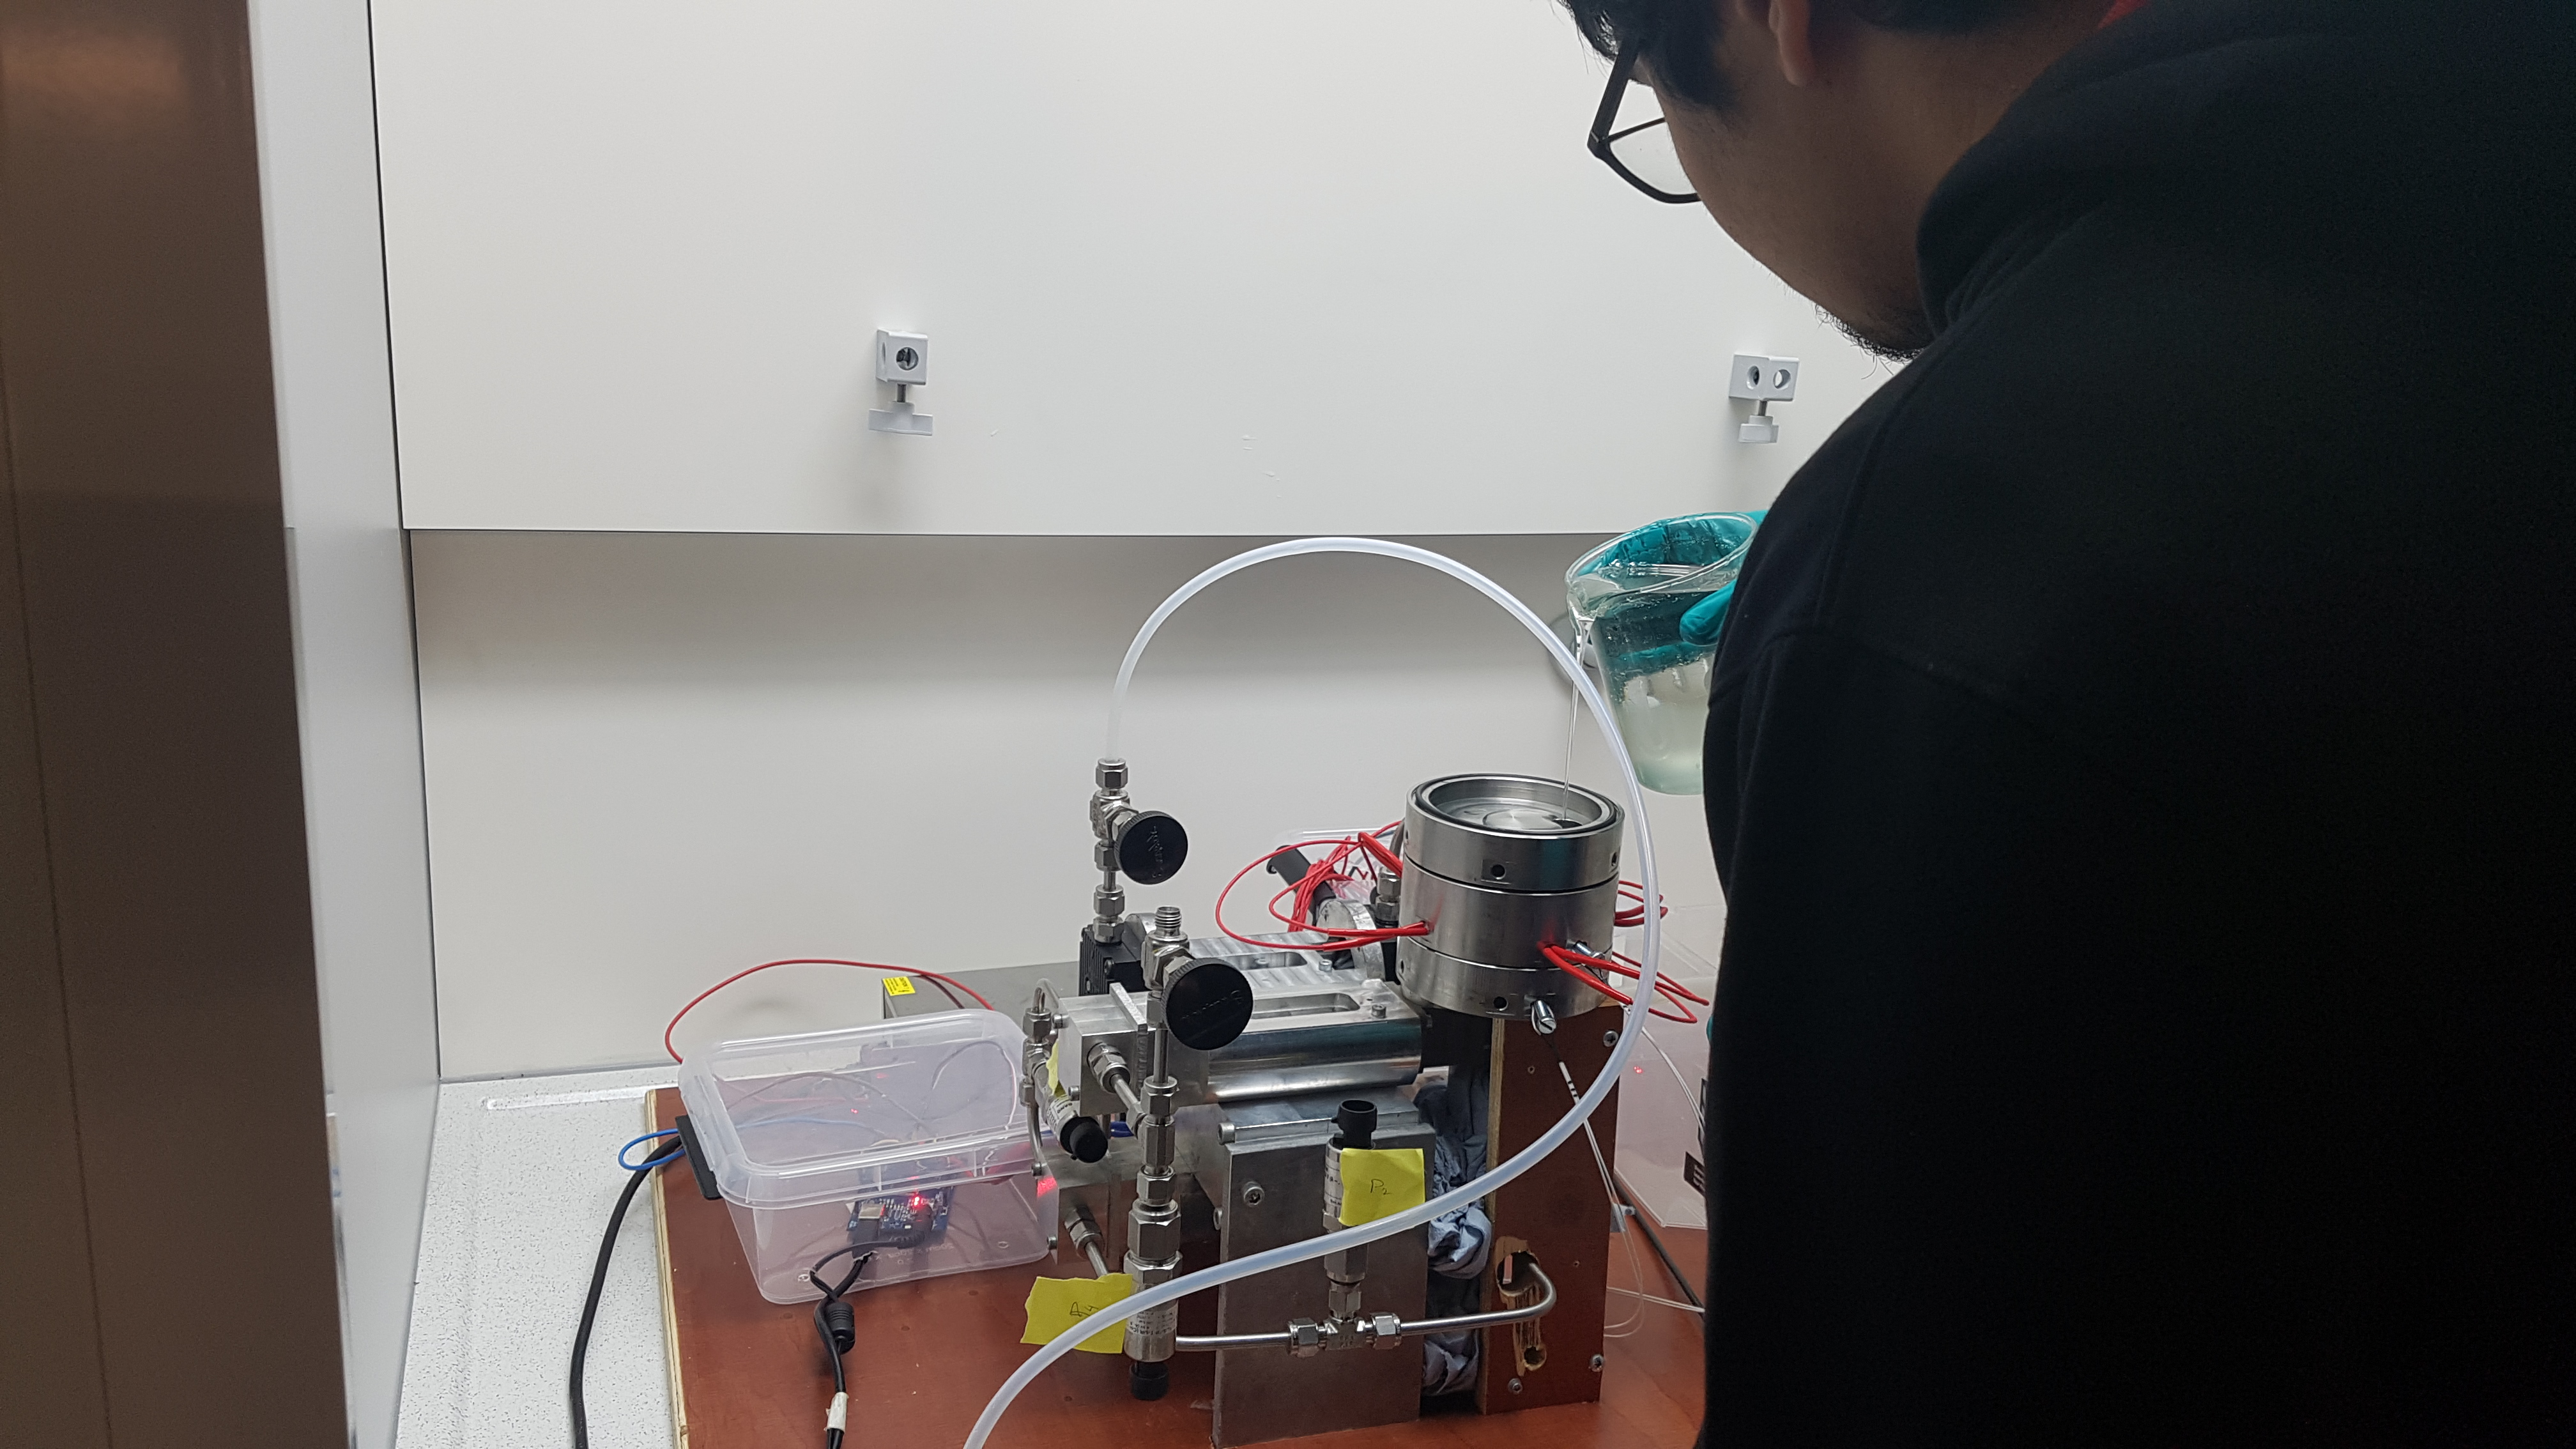
\includegraphics[scale = 0.1]{images/mywork/Sprint3/peiloading1.jpg}
    \caption{Loading PEI into the system}
    \label{fig:peiloading}
\end{figure}

It was observed that the PEI was so viscous that the PEI pump couldn't pump the normal PEI to the distributor. This was later inferred to be due to mainly two reasons :
\begin{itemize}
    \item Placement of the inlet nozzle in the extremes of the manifold - the inlet of the PEI flow from PEI pump to the DAC manifold was kept at the extreme nozzle. We know that there is significant pressure head loss when the length of pipe is very long. The solution for this was to cut the pipe length between DAC manifold and DAC distributor very short. The PEI inlet flow was shifted to the central nozzle as well for uniform distribution. 
    \item Using cold PEI - from previous reports we know that PEI becomes much less viscous at higher temperature. Hence, it wouldn't have much resistance in pumping the system up. 
\end{itemize} 


On rectifying the mistake and setting the heater temperature at 80 \degree C. The PEI was able to flow perfectly across the system and making it a continuous system. However, some observations were made that wasn't desirable which shall be elaborated more in the next Section of the report. 

\subsubsection{DAC System V1.1 breaks and issues}
\label{sec:breakdown}

During the entire runtime of the DAC System V1.1 we face many issues with broken 3D print components and leaks from the system. On further brainstorming and the cause of these issues and solutions were discussed. Some of the main issues that the system faced was : 

\begin{itemize}
    \item \textbf{Improper component geometry :} Due to improper design, improper assumptions and improper orientation. This can be seen in the following Figure \ref{fig:flowanomaly} below.
    \item \textbf{Desorber vibrations :} Due to improper orientation of the desorber chamber. At times, we could see that desorber would vibrate a lot out position and the chamber might come out of the vacuum condition. This caused a lot of PEI spills and was a pain to clean up as seen in Figure \ref{fig:leakingcompressor}. 
    
    \begin{figure}[H]
        \centering
        \begin{minipage}{.5\textwidth}
        \centering
        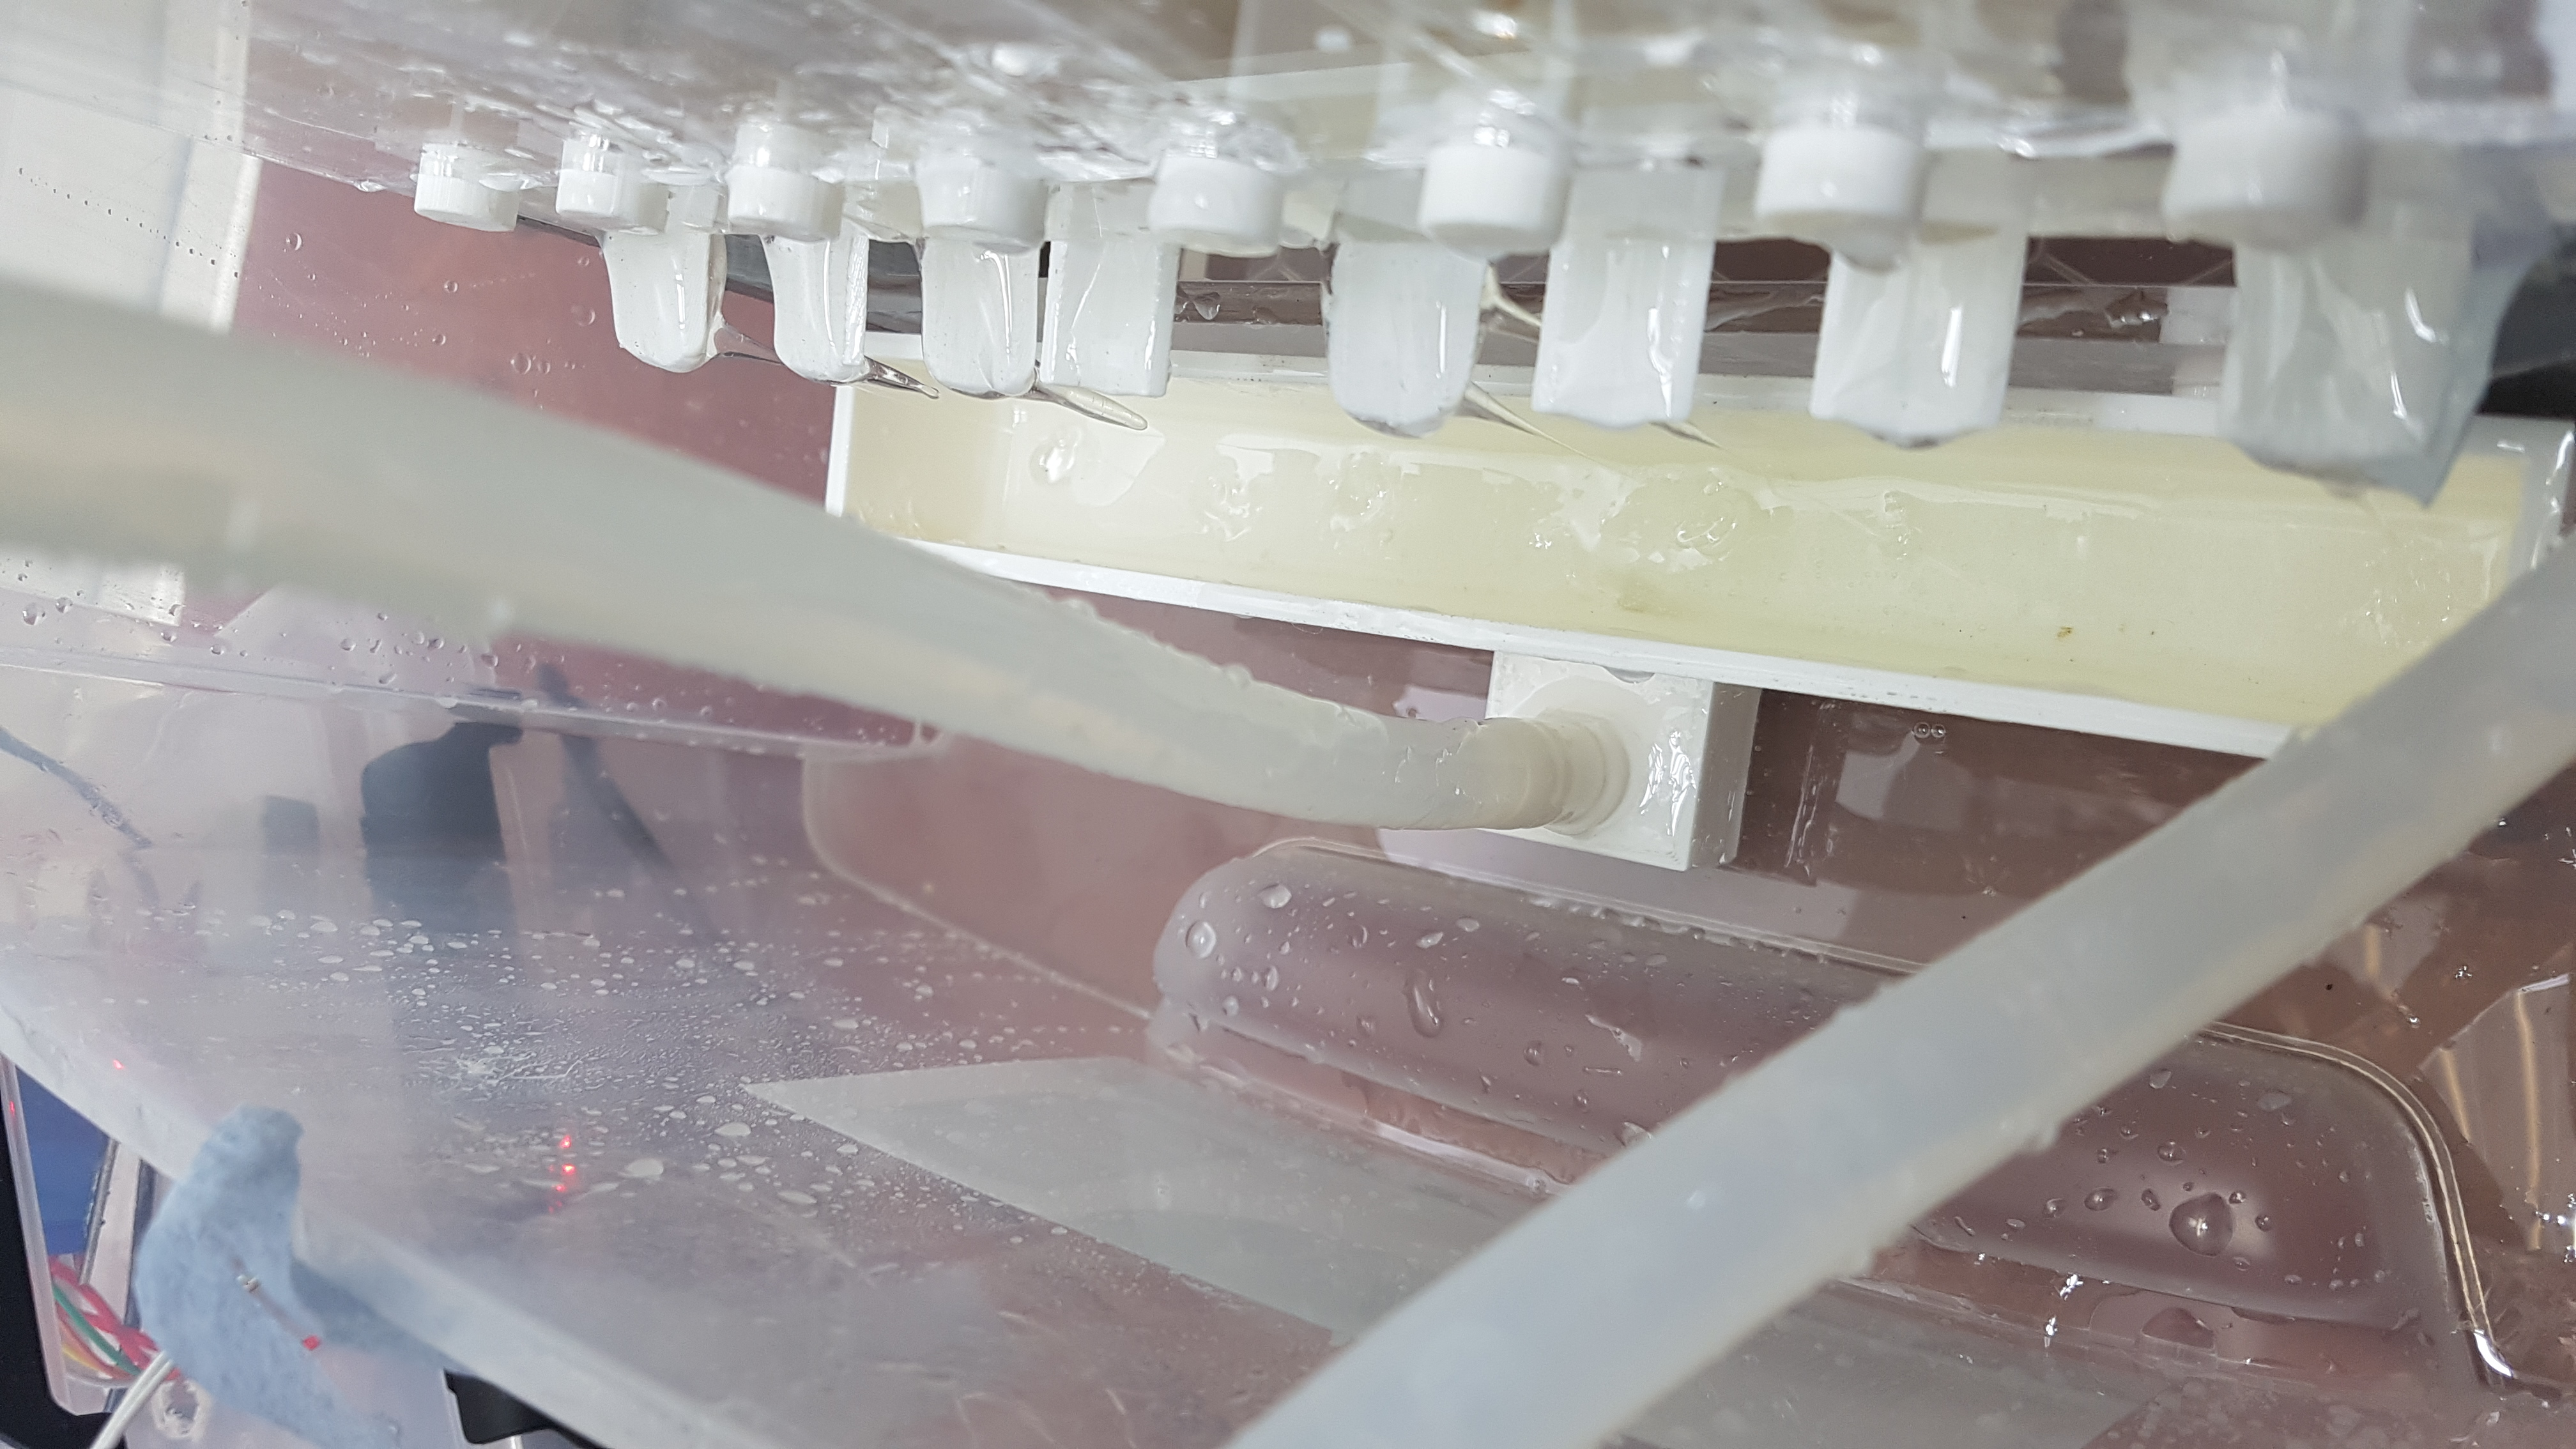
\includegraphics[width=0.9\linewidth, angle = 270]{images/mywork/Sprint3/flowanomaly.jpg}
        \captionof{figure}{Flow out of the DAC collector}
         \label{fig:flowanomaly}
    \end{minipage}%
    \begin{minipage}{.5\textwidth}
        \centering
        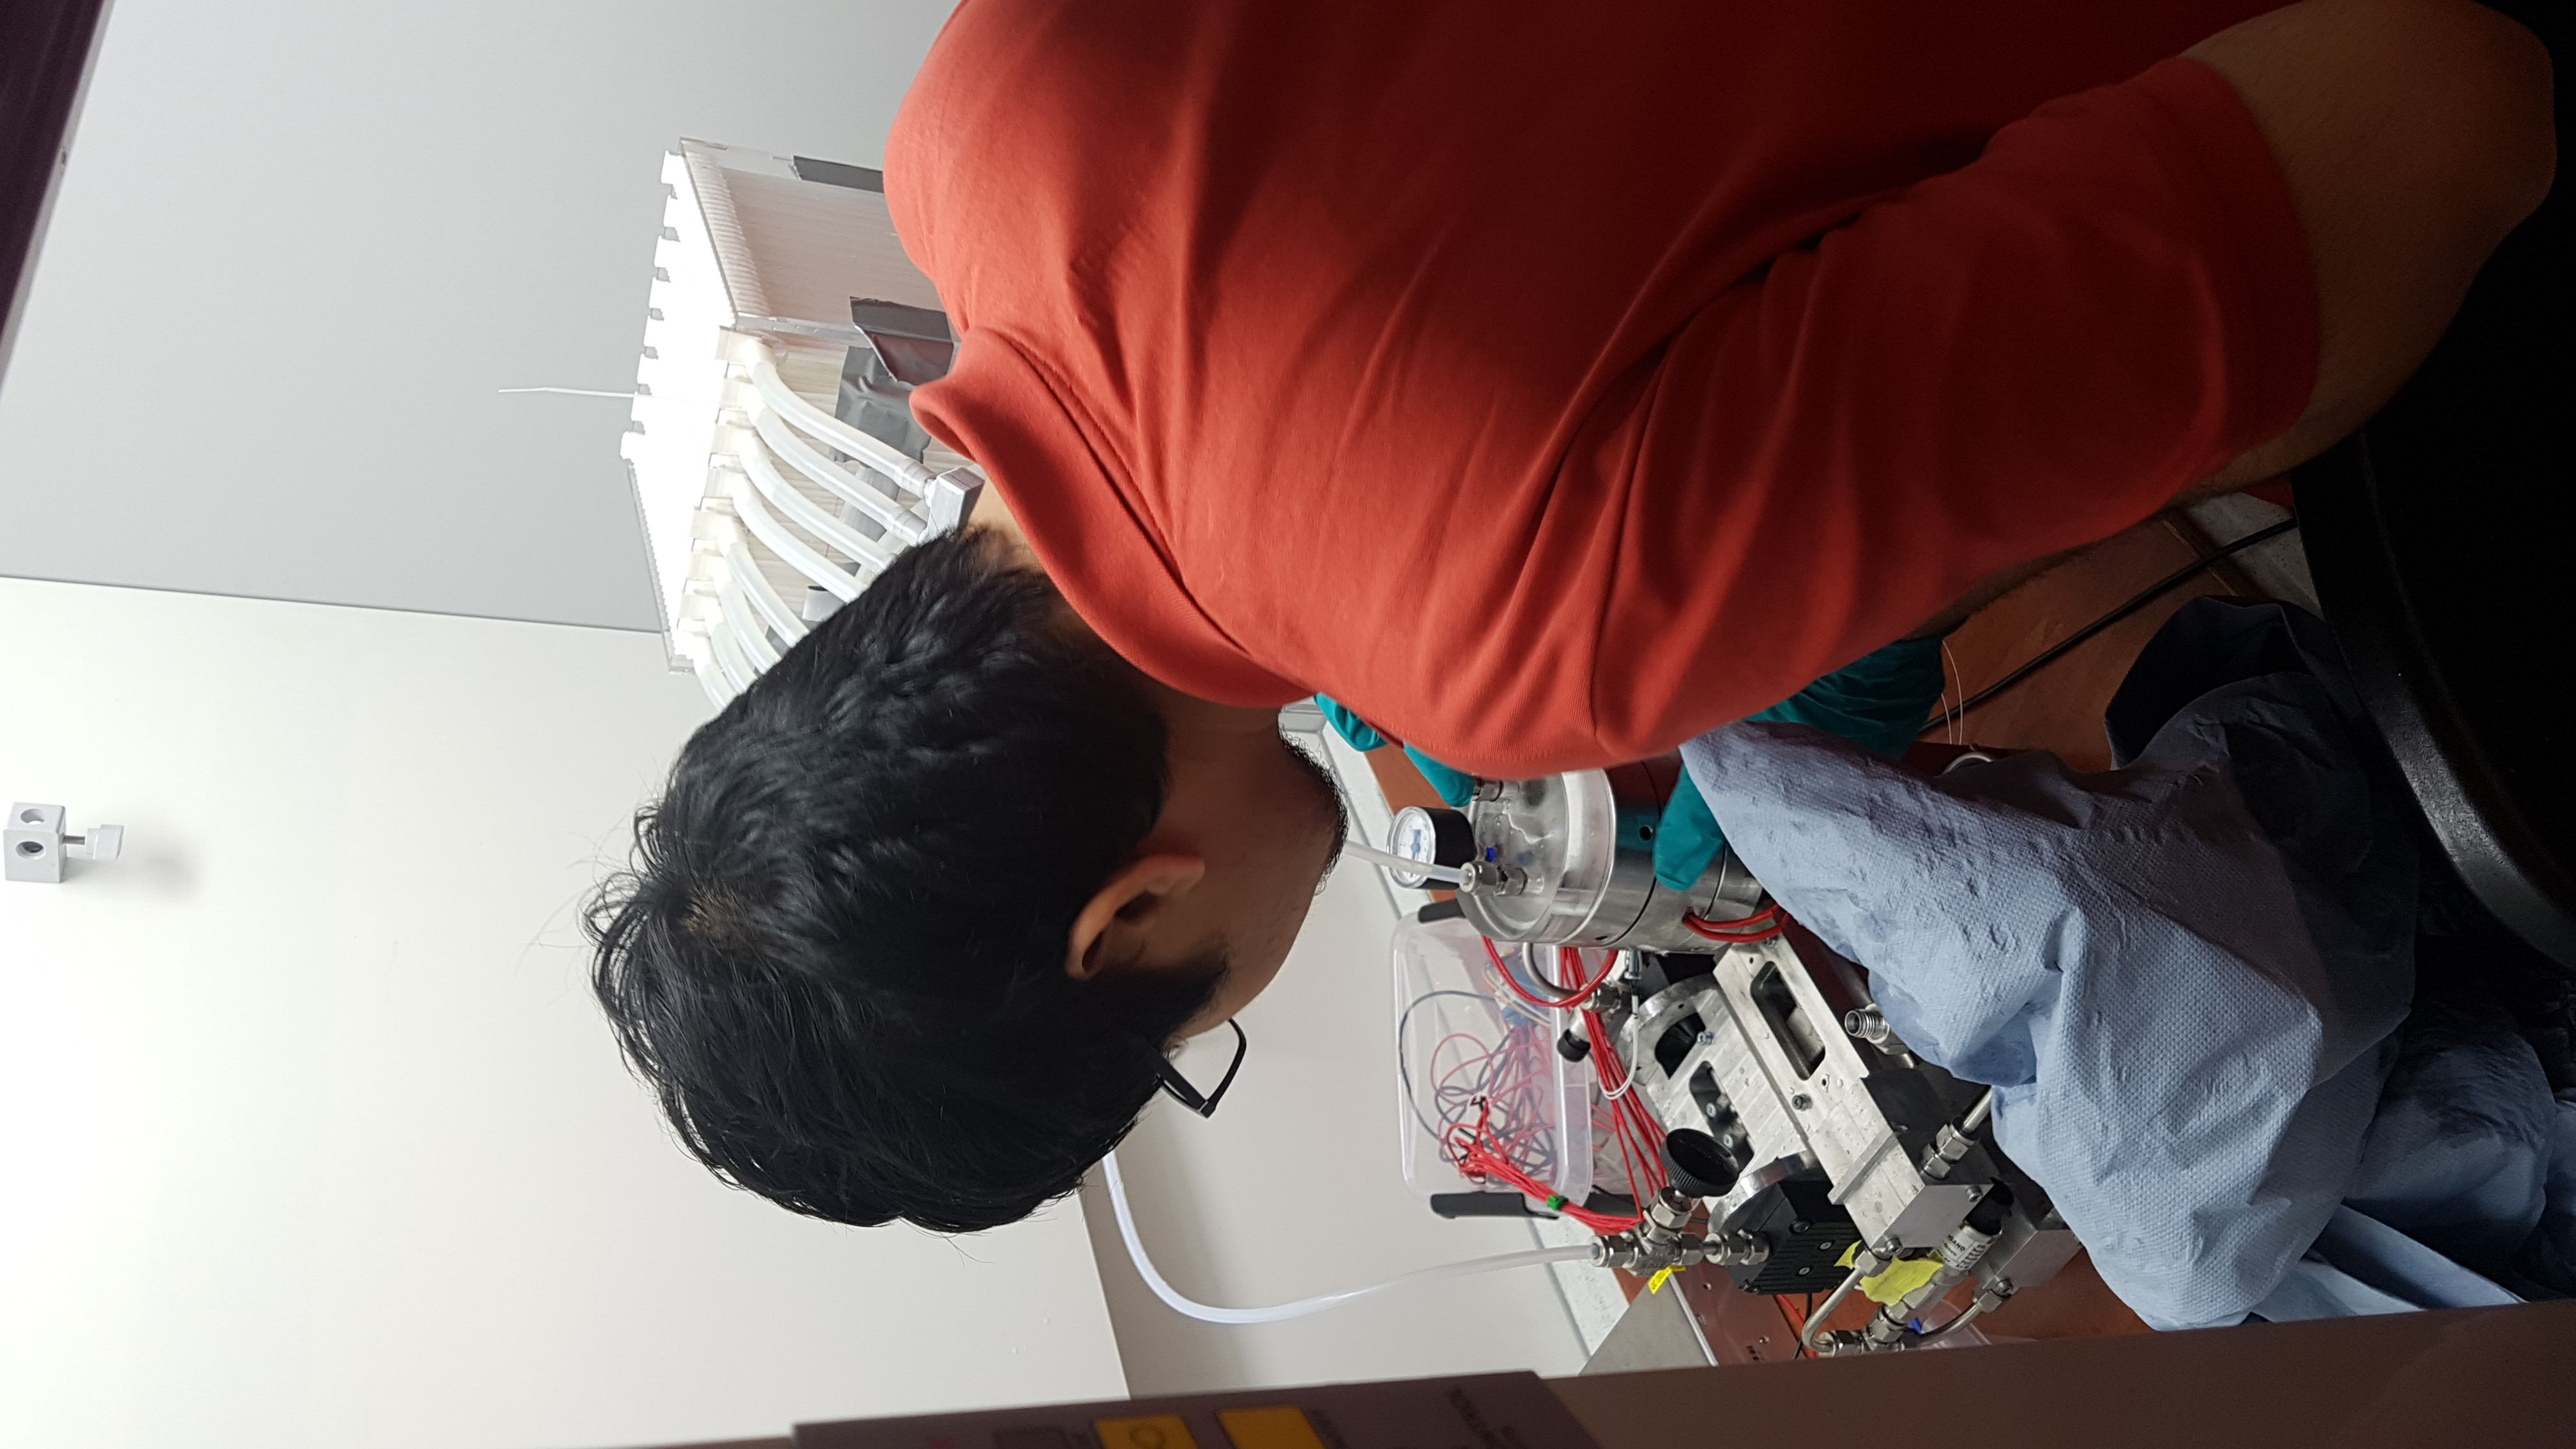
\includegraphics[width=0.9\linewidth, angle = 270]{images/mywork/Sprint3/messysystem.jpeg}
        \captionof{figure}{Leaking desorber chamber}
        \label{fig:leakingcompressor}
    \end{minipage}
    \end{figure}
    
    \item \textbf{Hot PEI reacts with PLA :}
    \label{sec:hotpei} During the Sprint 3 - a lot of our 3D prints were breaking like the collector bucket nozzle, the manifold nozzle and the distributor. At first, we inferred it was because of some accident or because of the way layers were set on the 3D printer making it a weak structure. However, on further studying it by putting a PLA piece in hot PEI. We found out that the PLA piece got completely dissolved within 30 minutes itself. Hence, it was decided that we have to look into other way to make the different DAC components.   
    
\end{itemize}


\subsection{Sprint 4 - $4^{th}$ November - $25^{th}$ November}

During the $4^{th}$ phase of the internship, we laid the foundations for the DAC V2.0 system. We had addressed the issues we faced while running the DAC V1.1 system for long hours as elaborated in Section \ref{sec:breakdown}. We also changed the material used for prototyping and the type of the manufacturing the prototype as well which is from 3D printing to SLS printing. 

\subsubsection{Design changes}
In order to rectify the geometry mistakes we changed the geometry of some of the DAC components. The design of the components were changed in order to accommodate these changes which will be elaborated more below :

\begin{itemize}
    \item \textbf{Manifold :} in-order to make the flow uniform and make sure that all the PEI that has absorbed $CO_2$ is distributed uniformly, the internals of the manifold is made in the form of a cyclinder than its cuboidal shape. The internal diameters of the manifold nozzles were also changed to 6mm diameter. As seen in Figure \ref{fig:newmani}, the new manifold has a Swagelok connection to the manifold that supplies the TEPA inlet, unlike in the old manifold as seen in Figure \ref{fig:oldmani}.
    
    
        \begin{figure}[H]
        \centering
        \begin{minipage}{.5\textwidth}
        \centering
        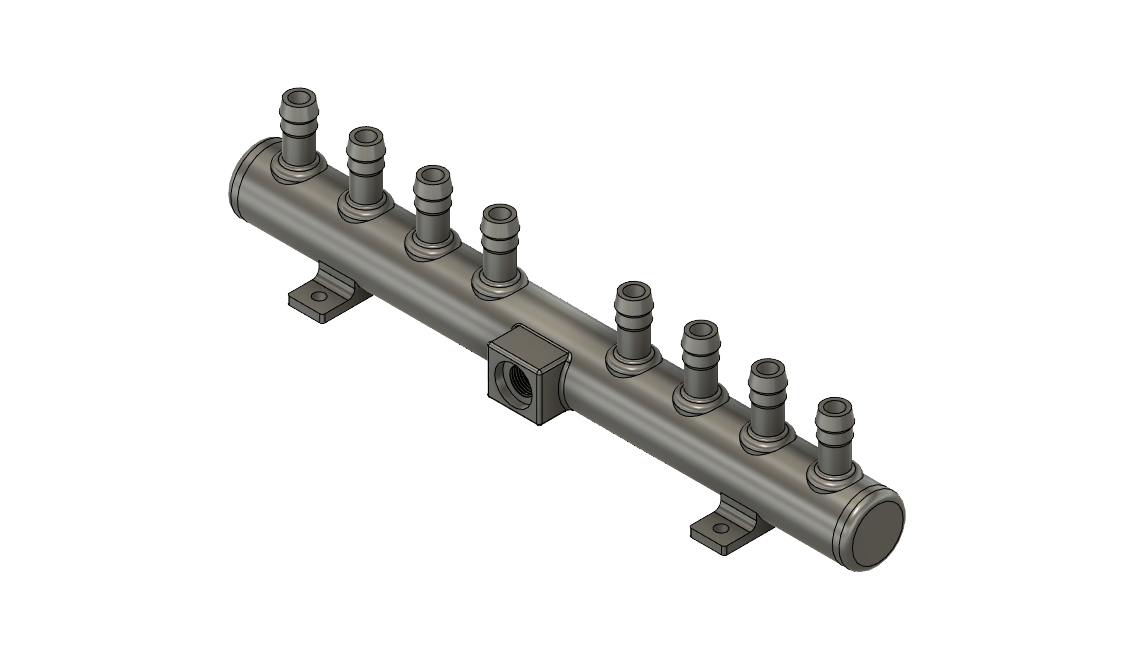
\includegraphics[width=\linewidth]{images/mywork/Sprint4/Manifold_main.png}
        \captionof{figure}{DAV V2.0 Manifold}
         \label{fig:newmani}
    \end{minipage}%
    \begin{minipage}{.5\textwidth}
        \centering
        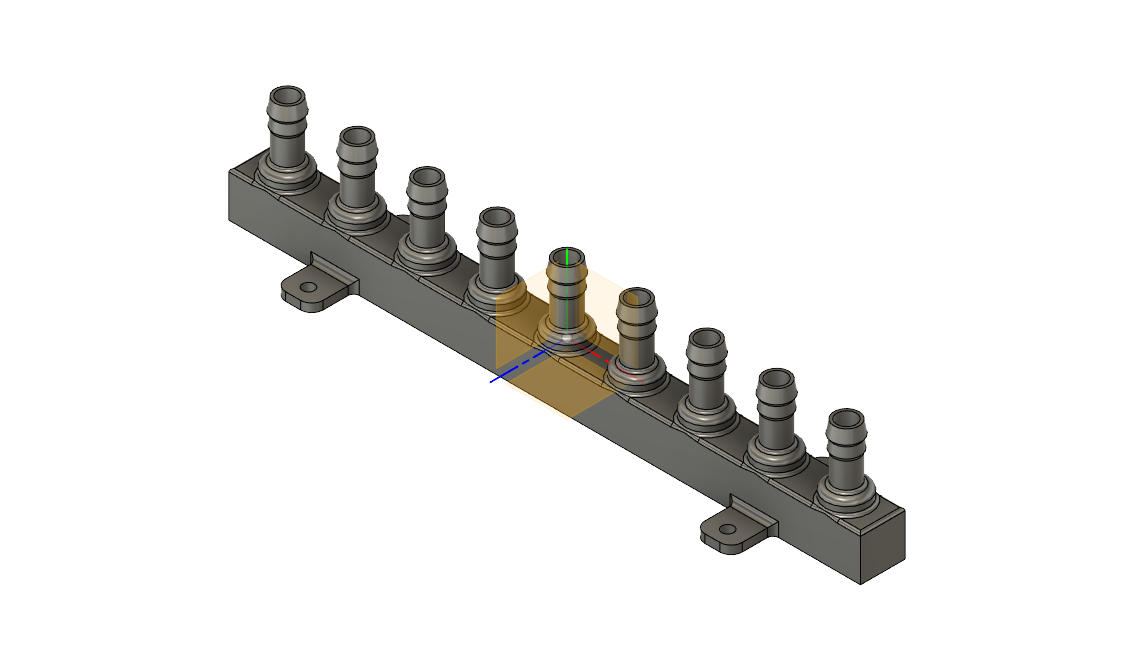
\includegraphics[width=\linewidth]{images/mywork/Sprint4/Manifold_old.png}
        \captionof{figure}{DAV V1.1 Manifold}
        \label{fig:oldmani}
    \end{minipage}
    \end{figure}
    
    \item \textbf{Collector :} In order to address the undesired PEI flowing out of the collector. We changed the outlet into a bent nozzle as seen in Figure \ref{fig:newcoll}. I wanted to give more support for the DAC channel plates and hold it with a grip like the DAC distributor system holds it together. This was done by creating slots which can keep the . By doing so, the DAC channels will be held in place rather than in an haphazard manner like in the last system where we had to drill holes on the PMMA sheets and added nails to keep them in place. 
    
    \begin{figure}[H]
        \centering
        \begin{minipage}{.5\textwidth}
        \centering
        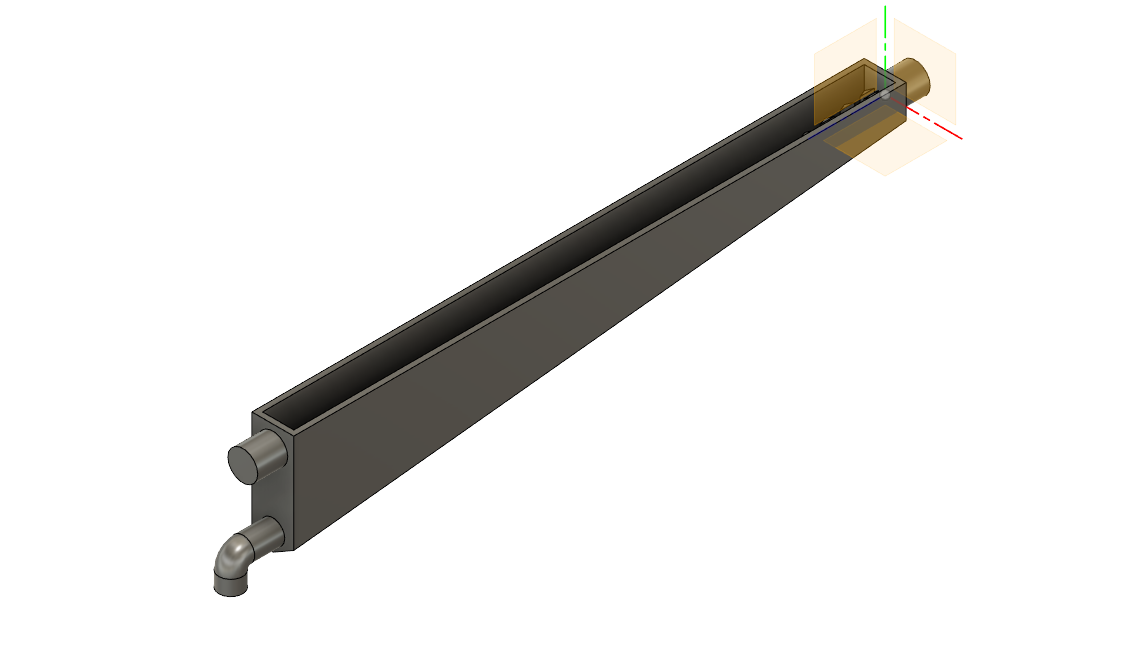
\includegraphics[width=\linewidth]{images/mywork/Sprint4/Collector_main.png}
        \captionof{figure}{DAV V2.0 Collector}
         \label{fig:newcoll}
    \end{minipage}%
    \begin{minipage}{.5\textwidth}
        \centering
        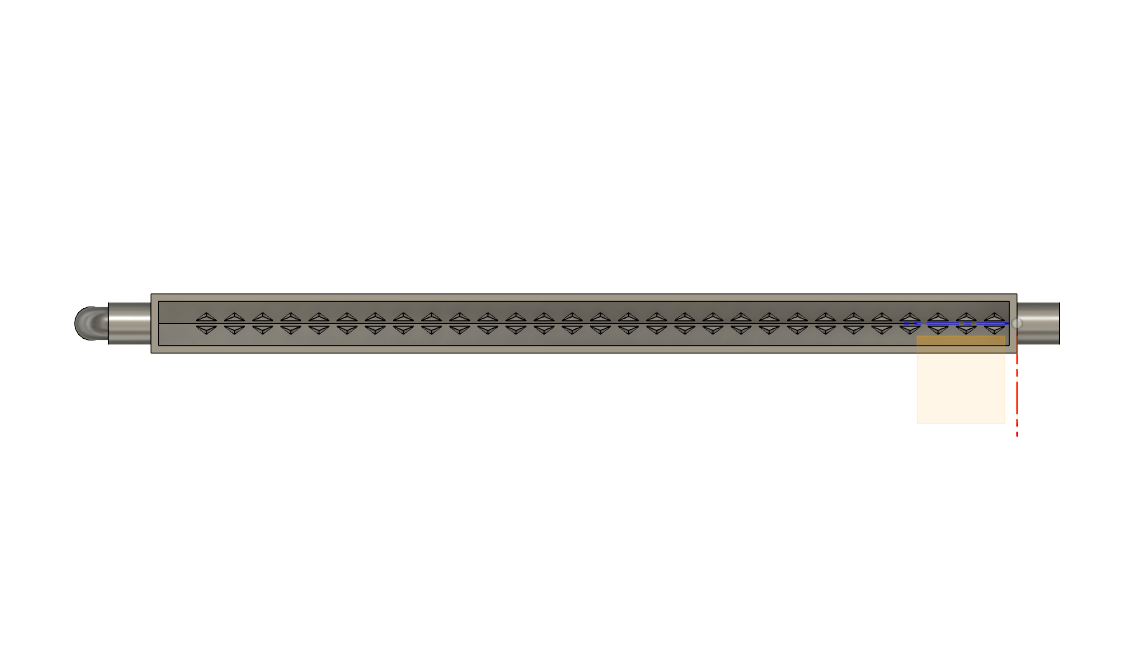
\includegraphics[width=\linewidth]{images/mywork/Sprint4/Collector_new_top.png}
        \captionof{figure}{DAV V2.0 Collector top view}
        \label{fig:newcolltop}
    \end{minipage}
    \end{figure}
    
    
    \begin{figure}[H]
        \centering
        \begin{minipage}{.5\textwidth}
        \centering
        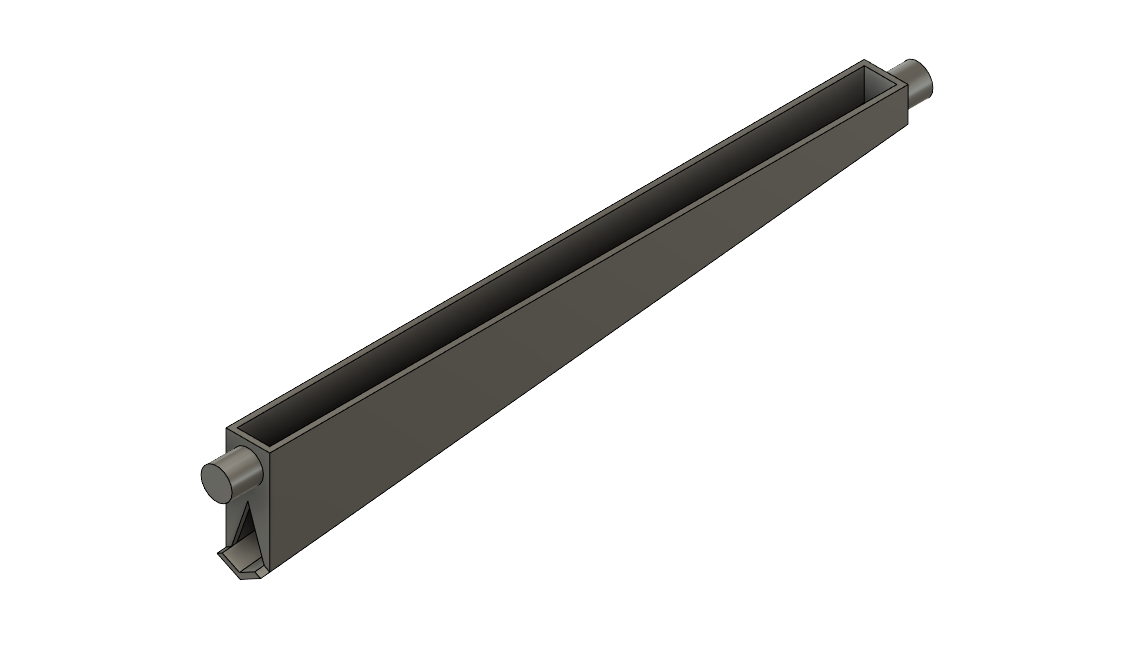
\includegraphics[width=\linewidth]{images/mywork/Sprint4/Collector_old.png}
        \captionof{figure}{DAV V1.1 Collector}
         \label{fig:oldcoll}
    \end{minipage}%
    \begin{minipage}{.5\textwidth}
        \centering
        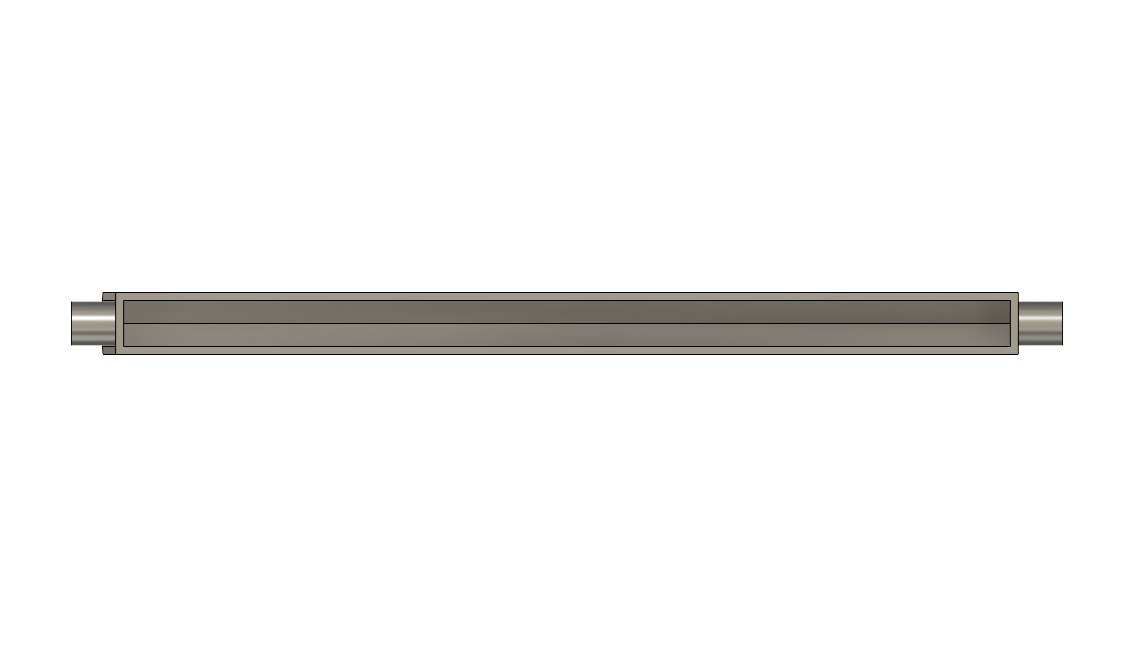
\includegraphics[width=\linewidth]{images/mywork/Sprint4/Collector_old_top.png}
        \captionof{figure}{DAV V1.1 Collector top view}
        \label{fig:oldcolltop}
    \end{minipage}
    \end{figure}
    
    
        Comparing Figure \ref{fig:newcoll} and Figure \ref{fig:oldcoll}, we can see the new nozzle extension in the new DAC V2.0 Collector. On observing Figure \ref{fig:oldcolltop} and Figure \ref{fig:newcolltop} we can see the extra slots added to hold the DAC polypropelene channels in place. It also eliminates the need for nails for fixing the polypropelene channels in place as in DAC system V1.1. 
        
        \item \textbf{Distributor :} The distributor had very less design changes and with respect to design. The old distributor design worked perfectly but in-order to make it better. The cross section of the distributor is changed from a cylindrical cross section to a rectangular cross-section for uniform distribution of TEPA or PEI as per Mr. Leonard Schrug's recommendations. The internal diameter was also changed to 6 mm. Since, the new prototyping method was using SLS method, I had made a M6 screw threaded hole so that after machining, the manufactures can clear all the pieces inside the chamber. Once we receive the distributors, we close the holes using M6 screws. 
        
        \begin{figure}[H]
        \centering
        \begin{minipage}{.5\textwidth}
        \centering
        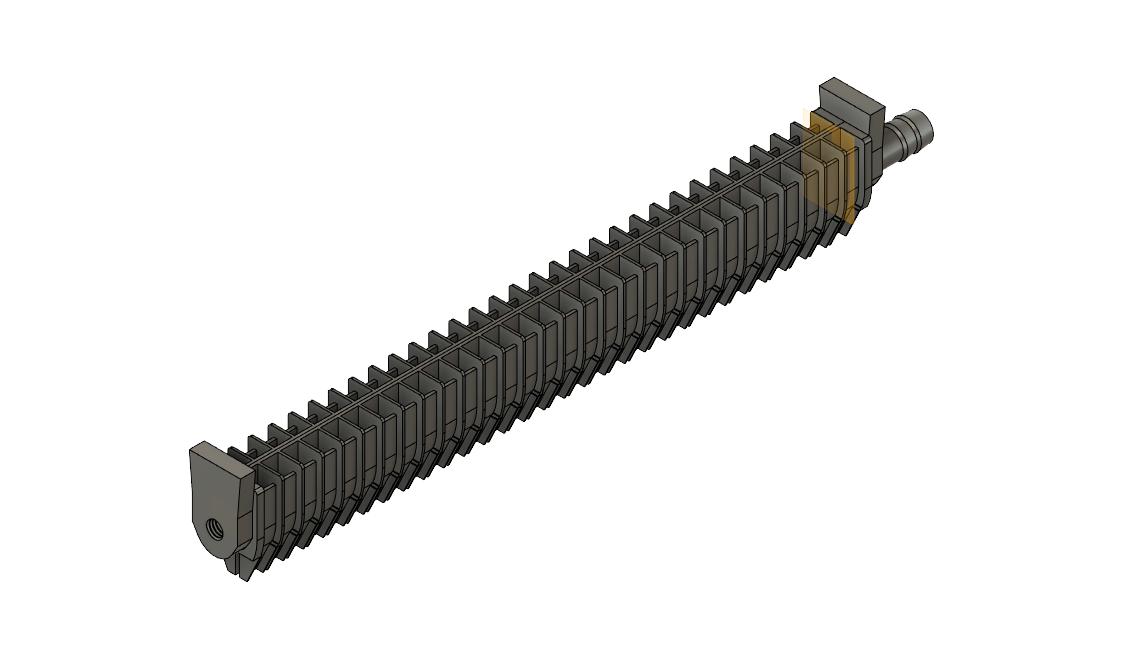
\includegraphics[width=\linewidth]{images/mywork/Sprint4/Distributor_main.png}
        \captionof{figure}{DAC V2.0 Distributor}
         \label{fig:2dis}
    \end{minipage}%
    \begin{minipage}{.5\textwidth}
        \centering
        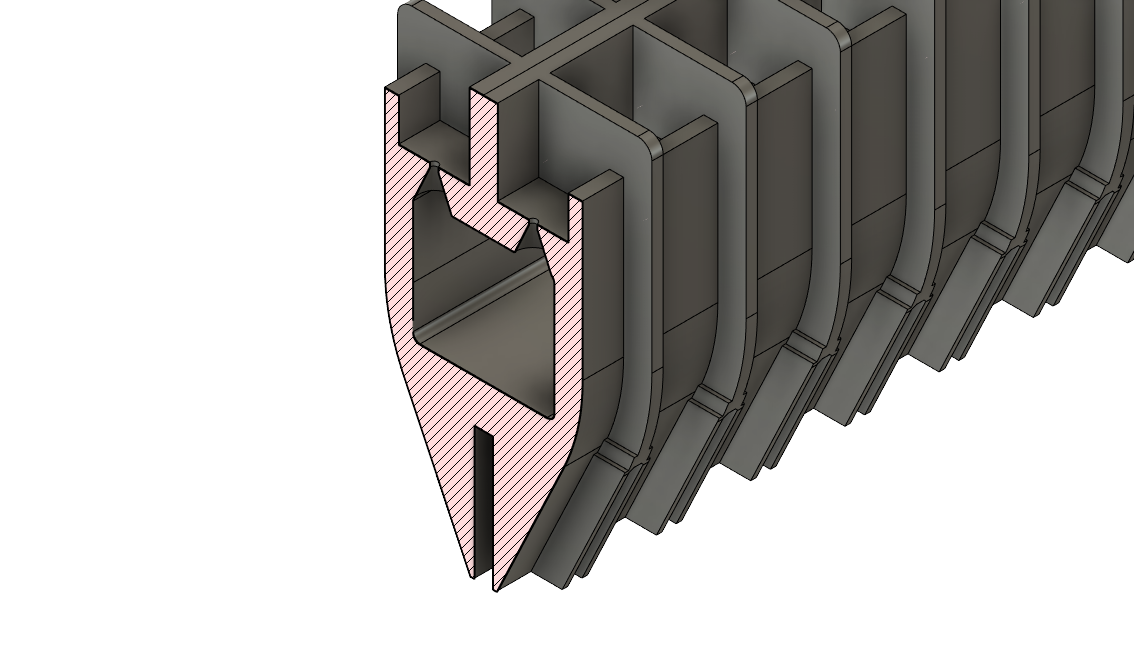
\includegraphics[width=\linewidth]{images/mywork/Sprint4/newdiscross.png}
        \captionof{figure}{DAC V2.0 Distributor cross section}
        \label{fig:2discross}
    \end{minipage}
    \end{figure}
    
    
    \begin{figure}[H]
        \centering
        \begin{minipage}{.5\textwidth}
        \centering
        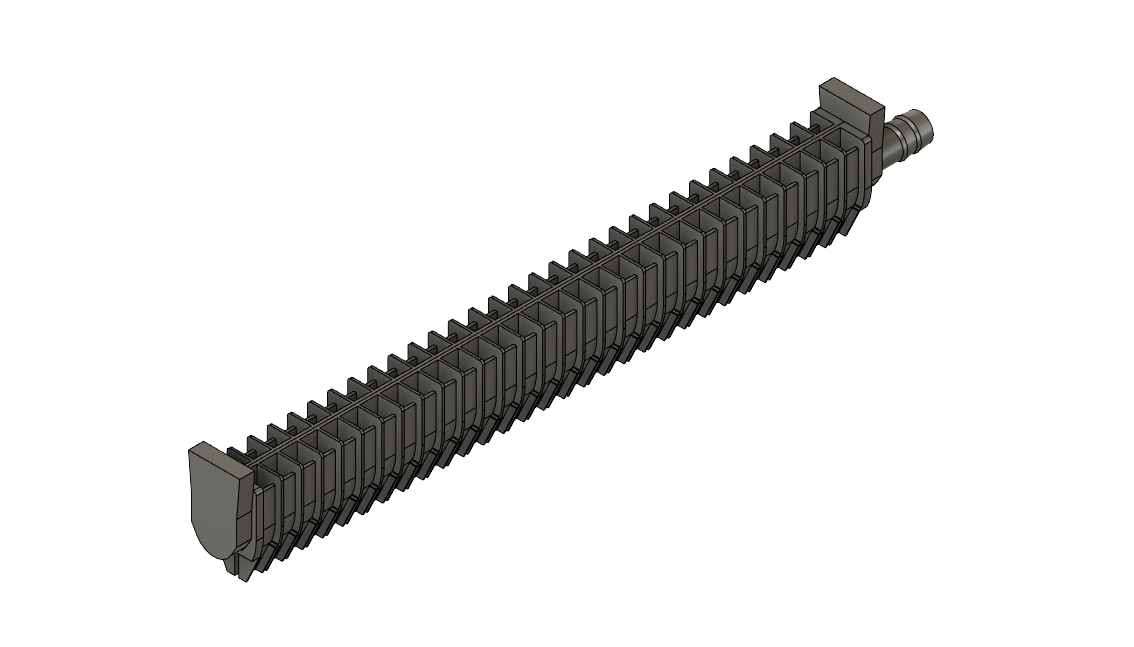
\includegraphics[width=\linewidth]{images/mywork/Sprint4/Distributor_old.png}
        \captionof{figure}{DAC V1.1 Distributor}
         \label{fig:1dis}
    \end{minipage}%
    \begin{minipage}{.5\textwidth}
        \centering
        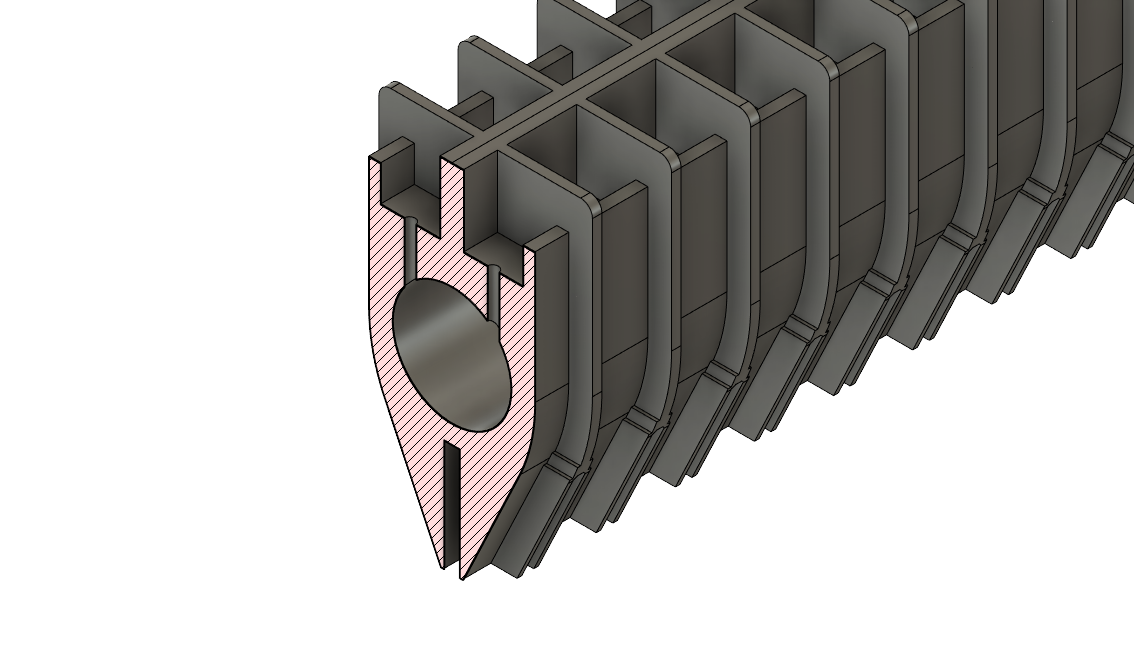
\includegraphics[width=\linewidth]{images/mywork/Sprint4/olddiscross.png}
        \captionof{figure}{DAC V1.1 Distributor cross section}
        \label{fig:1discross}
    \end{minipage}
    \end{figure}
    
    
    As seen in Figure \ref{fig:2dis}, the new distributor component has a M6 screw thread hole. The comparision of the cross sections difference between the new and the old design can be seen in Figure \ref{fig:2discross} and Figure \ref{fig:1discross}. In the above Figures, we can also see that the nozzle designs have been changed as well for better distribution and smaller nozzle diameter. 
    
\end{itemize}

\subsubsection{Material and production changes}

We have seen in Section \ref{sec:hotpei} that hot PEI reacts with the 3D printing material PLA. Hence, this caused many DAC components like the distributors, the nozzles of the collector bucket and manifold to break due to chemical degradation. This was later confirmed by Wino Spix when he reacted hot PEI with PLA material in a stand alone environment. In order to overcome this issue, we looked into various other ways of prototyping and thanks to Leanord's recommendation. It was decided to go for SLS printing with the prototype material being nylon. We tested the SLS material first to see its reaction with TEPA since it is known that TEPA is more reactive in nature. Besides some discoloration due to the porus nature of nylon. The material was still intact after hours of exposure to TEPA. Hence, prototyping was done by SLS printing using nylon material.    


\subsubsection{Component changes}

It was decided to remove or change some components of the DAC system in order to improve the system's efficiency or make it easier to see the process occurring. Some of the changes that we have done in for the new DAC V2.0 system are as follows : 

\begin{itemize}
    \item \textbf{LIS fabricated compressor :} In DAC V1.1 system, we had used a compressor system that was manufactured by the previous LISForce team but as we seen in Section \ref{sec:faultycomp} and in Figure \ref{fig:psensor} that the compressor system couldn't meet the desired pressure of 50 bar. Hence, the compressor system was removed and a entirely new vacuum pump is used to maintain vacuum conditions in the new DAC desorber system. 
    
    \item \textbf{Si tubing :} The Si tubing in the DAC V1.1 system was removed and decided to implement PTFE tubing for the flow of TEPA/PEI across the various DAC components. It is known that PTFE tubes are more robust and can handle high temperatures as well. Thereby making it an ideal candidate for the system. 
    
    \item \textbf{Desorber column :} In Section \ref{sec:faultycomp} it is covered that the old desorbtion column can be seen in Figure \ref{fig:leaktest} and Figure \ref{fig:desorber}. This desorber had many issues such as moving due to vibrations of the compressor and PEI pump system which is elaborated in Section \ref{sec:breakdown}. In order to combat this issue and to make the system more isolated and transparent to see the distillation and desorbtion process occuring. A stainless steel distillation column is ordered from AliExpress and will be placed seperately from the whole DAC system.  
\end{itemize} 

\subsection{Sprint 5 - $25^{th}$ November - $9^{th}$ December}

In the $5^{th}$ phase of the internship. We started the assembly of the DAC V2.0 system and incorporating the above component changes as well. The idea for the DAC V2.0 system to become more robust and run for much longer run times than before without stopping or refilling and making it a closed system. The system should also have a continuous $CO_2$ out-stream as well that can be fed to the Fluid Machinery subsystem to pump it out at 50 bar.  


















\newpage
\section{Results \& Discussion }
\label{sec:results}

In this section, I shall cover the various results that I inferred while running the DAC V1.1 and DAC V2.0 system and discuss about my findings. In the first subsection we shall see how the DAC V1.1 system performed on running long times and the observations made while running it. In the second subsection we shall see how the DAC V2.0 system performed and the observations. 

\subsection{Observations from DAC V1.1 system}
\label{sec:dacv1.1obs}

\begin{figure}[H]
    \centering
    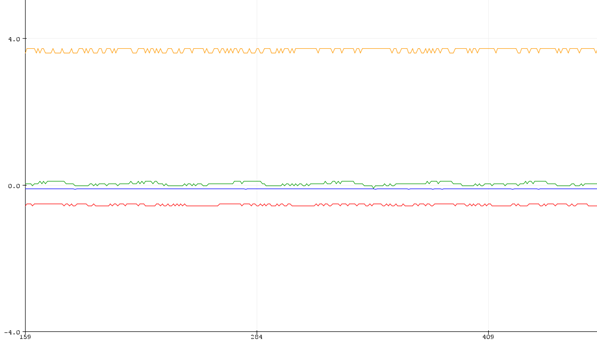
\includegraphics{images/mywork/Sprint2/pressuresensor.png}
    \caption{Pressure sensor outputs : Blue - P1, Red - P2, Green - P3 and Yellow - P4}
    \label{fig:psensor}
\end{figure}


The DAC V1.1 system desorber can be seen in Figure \ref{fig:desorber}. Since the desorber components were already present. I conducted leak tests and running the system for sometime to see if there is any issue with the PEI pump or the vacuum compressor. A point to note is that the system was designed to produce 50 bar pressure but on running it is found that the $3^{rd}$ stage of the compressor isn't pumping at the designed pressure ratio. This can be seen in the Figure \ref{fig:psensor} where the maxmium pressure output from the 4 stage compressor system is only below 4 bar pressure. It can also be seen that the P1,P2 and P3 are all around 0 bar pressure line which is not at all a desired output.
\bigbreak 
It was concluded to be due to leaks being present in the compressor system. So, leak tests were conducted as seen in Figure \ref{fig:leaktest} to see if there were any bubbles moving due to leaked gases at the Swagelok joints of the compressor system but the compressor had passed the leak test. On further examination by Pim (the LIS student who built the system), he pointed out that one of the Swagelok joints were in inch standards and not in the metric standards that we were using throughout the the system. 

\begin{figure}[H]
    \centering
    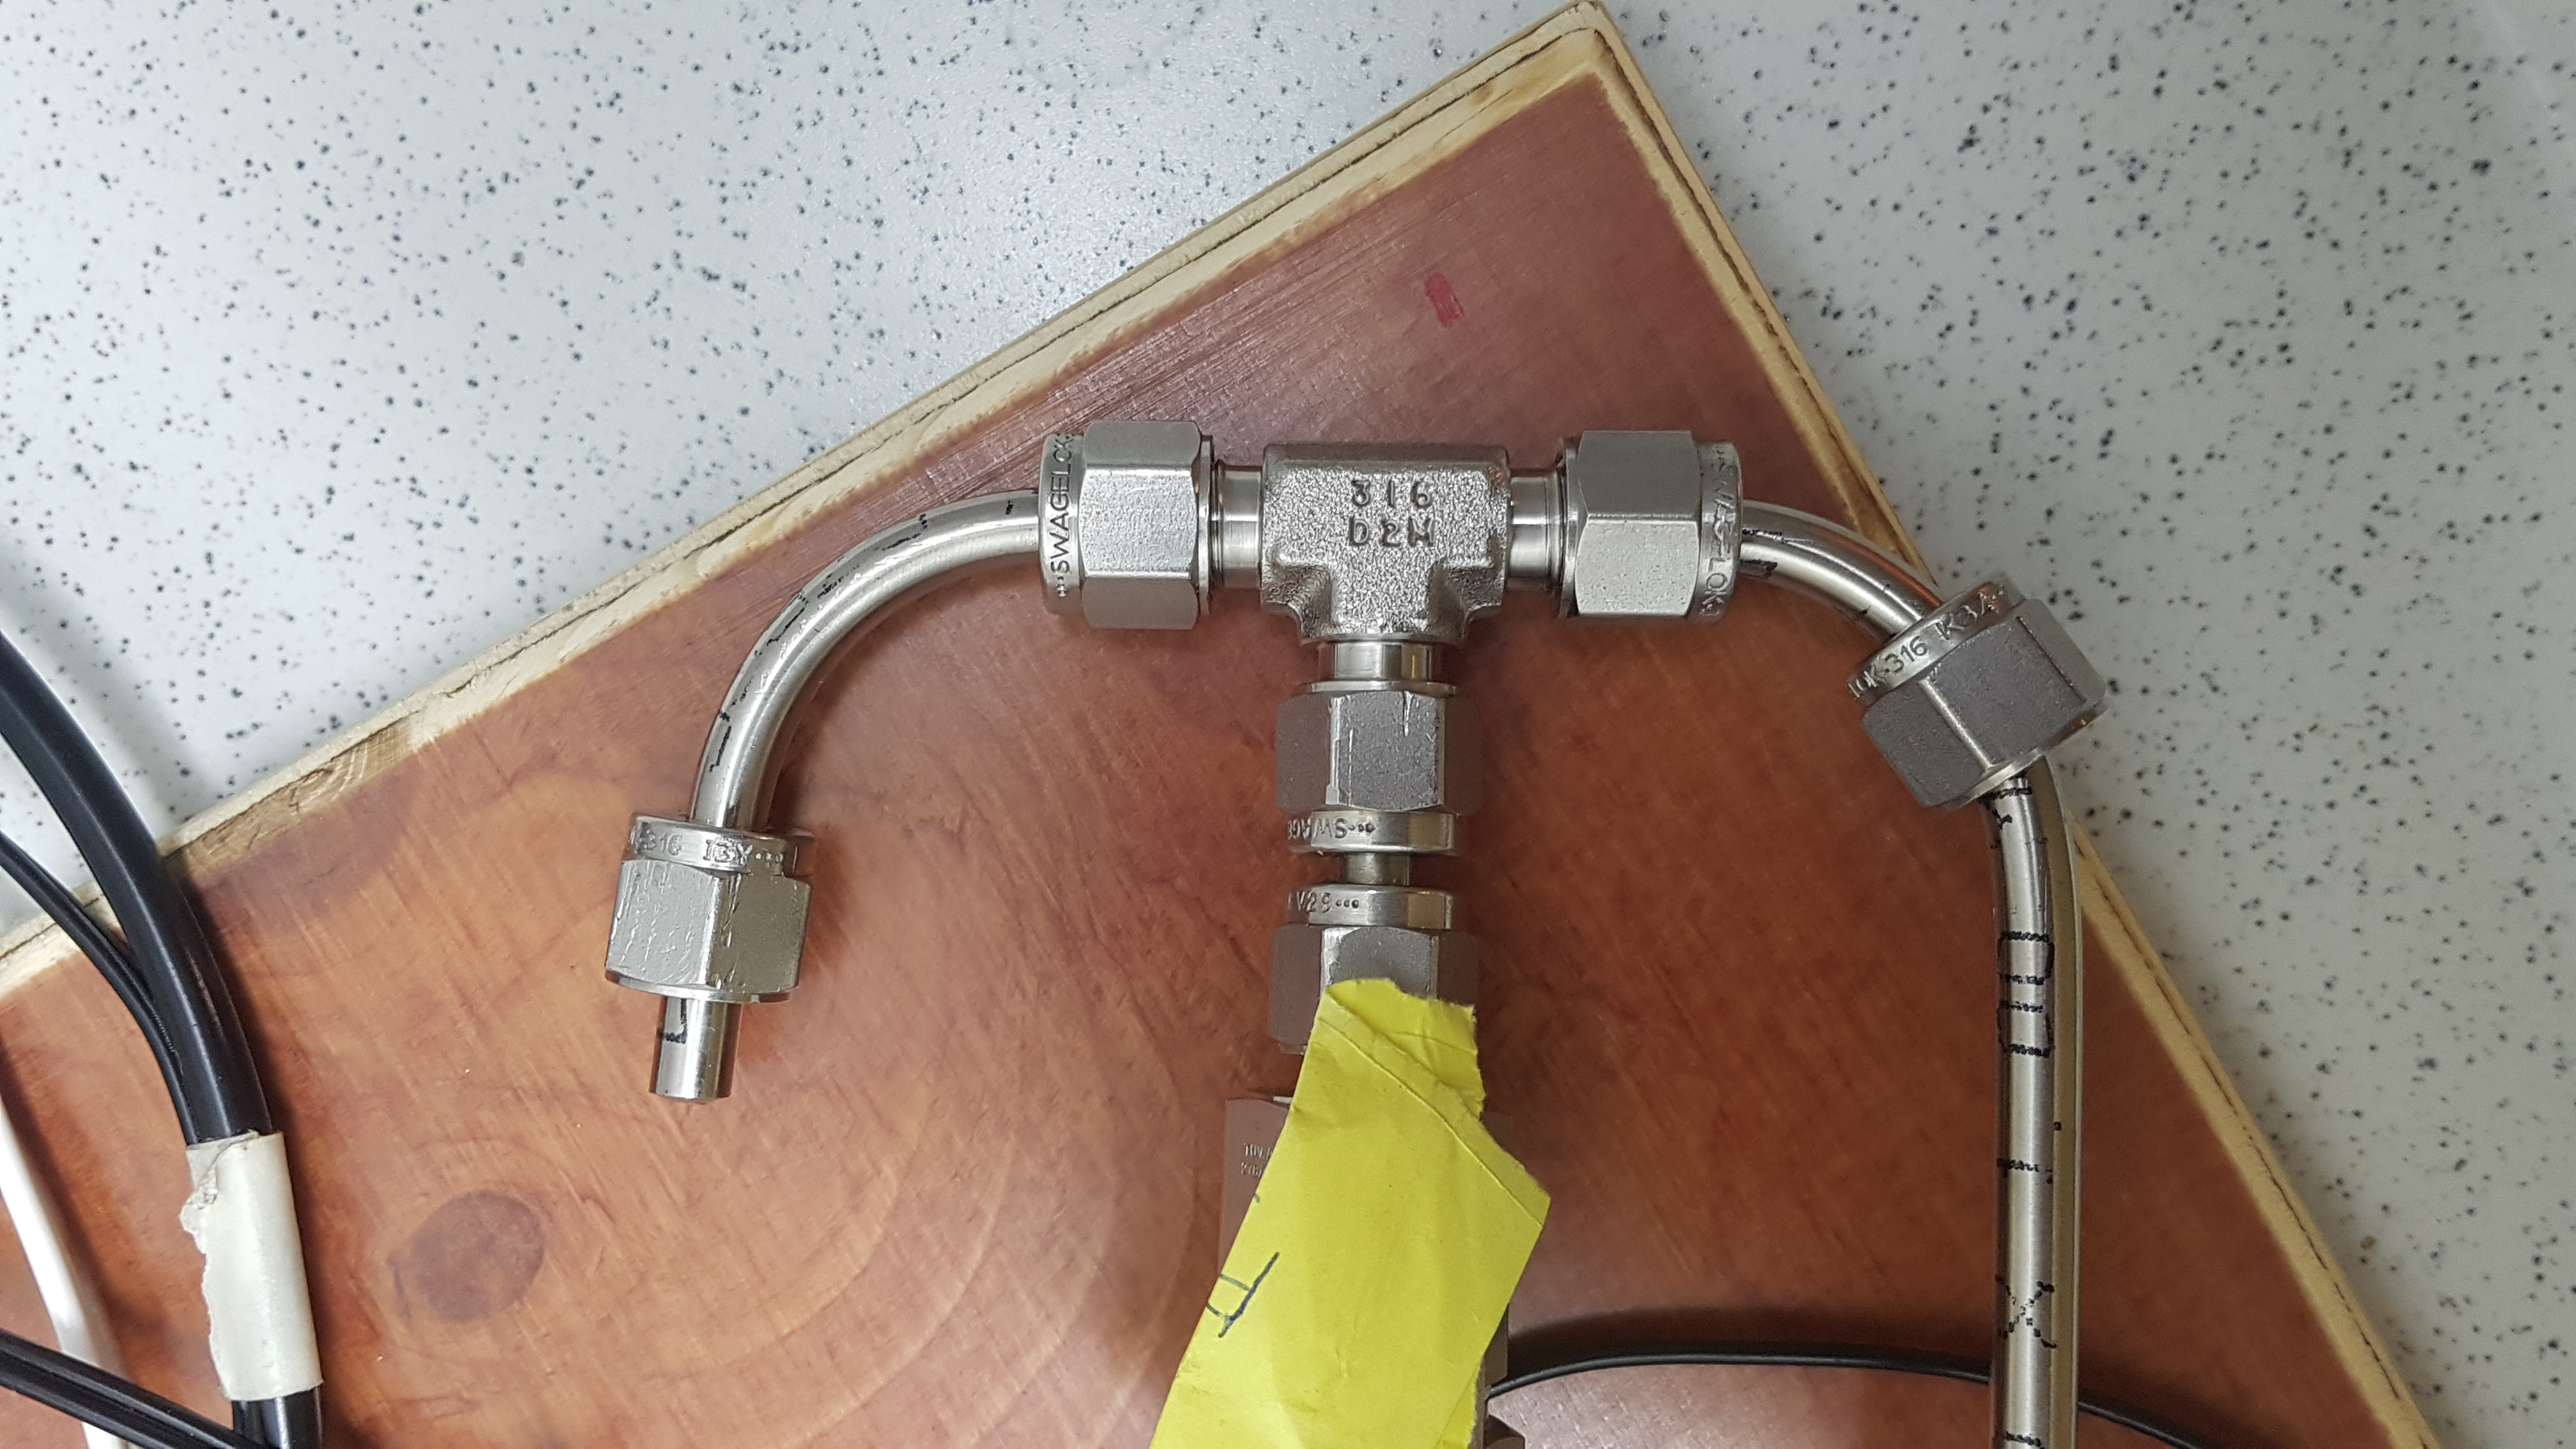
\includegraphics[scale = 0.07]{images/mywork/Sprint2/swagelok.jpg}
    \caption{Fixed the Swagelok joint}
    \label{fig:swagiss}
\end{figure}

In Figure \ref{fig:swagiss} the metric swagelok nuts are indicated by the small ring like feature below the octagonal feature used to hold the spanner. As seen in the figure, all the joints are fixed and made with metric bolts as per Pim's suggestion. Finally, the DAC system is complete and system is made to run. 

\subsubsection{Water testing}
\label{sec:watertest}

First, in order to ensure that there is no leaks in the system. Water was passed through the system - which was quite a bad idea since some of the water went into the vacuum compressor system. However, it turned out to be fine as all the water was cleared out. Once the water was all cleared out, PEI was passed into the system and made to run in the system and the system is closed. A proper flow of PEI was occurring with minimal to no leaks or spills. However, all the wiring was in a haphazard manner and I was told to make the electronic circuits into modules. Which was done using transparent boxes from Gamma store. Holes were created in the boxes so that wires can go from inside the box to outside the box and vice versa.
\bigbreak 
In Figure \ref{fig:dacsystem1.1}, we can see the complete DAC System V1.1 with all the components working together as one unit. In the background you can see the old broken down DAC System V1.0 of ZEF IV team. The following are the labelled components of the DAC system: 

\begin{itemize}
    \item 1 - DAC Absorber V1.1 
    \item 2 - DAC Desorber V1.1 
\end{itemize}

\begin{figure}[H]
    \centering
    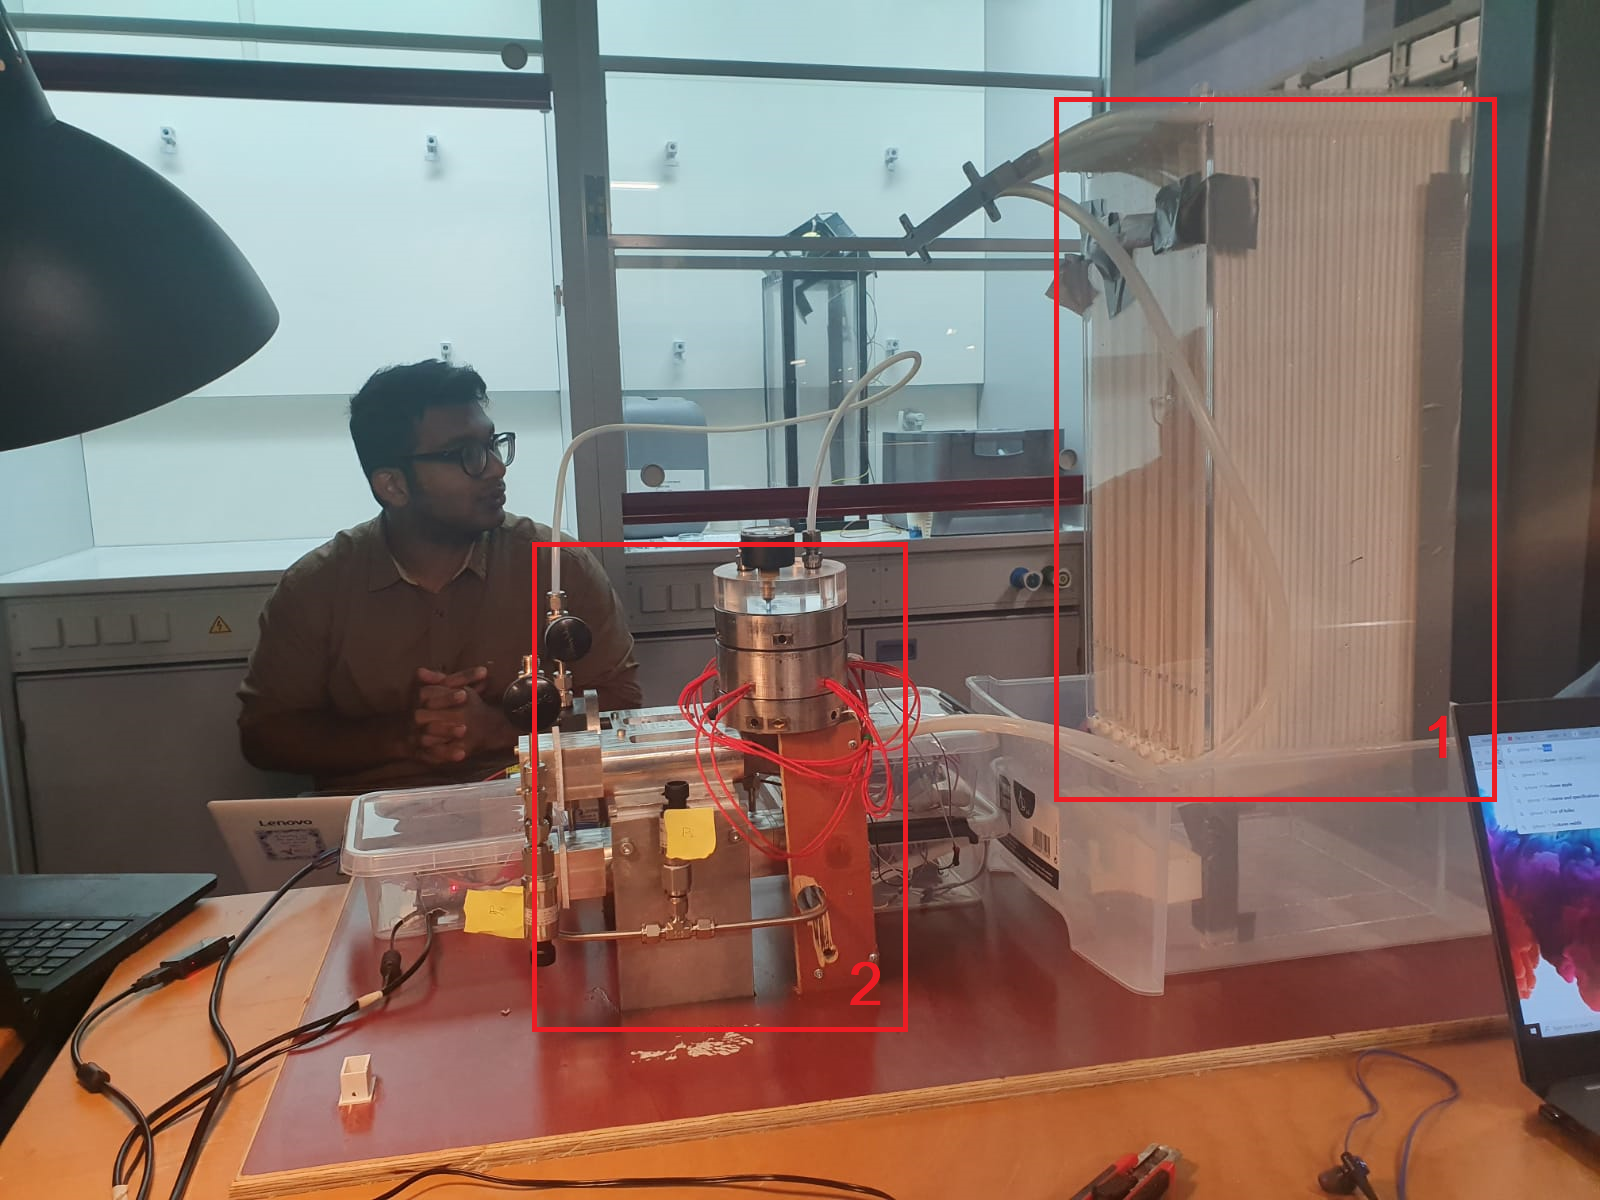
\includegraphics[scale = 0.45]{images/mywork/Sprint2/dacsystem1.png}
    \caption{The complete DAC System V1.1 }
    \label{fig:dacsystem1.1}
\end{figure}


\subsubsection{Running the DAC System V1.1 for long times with PEI}
\label{sec:obs}

We ran the DAC System V1.1 for about 7.23 hours cumulatively at varying RPMs of the PEI pump motor for various test conditions before the system broke. At first, we loaded PEI into the system from the desorbtion chamber without heating the desorbtion chamber. It can be seen in the Figure \ref{fig:peiloading}. This was done just to observe how PEI is flowing through the system. 

\begin{figure}[H]
    \centering
    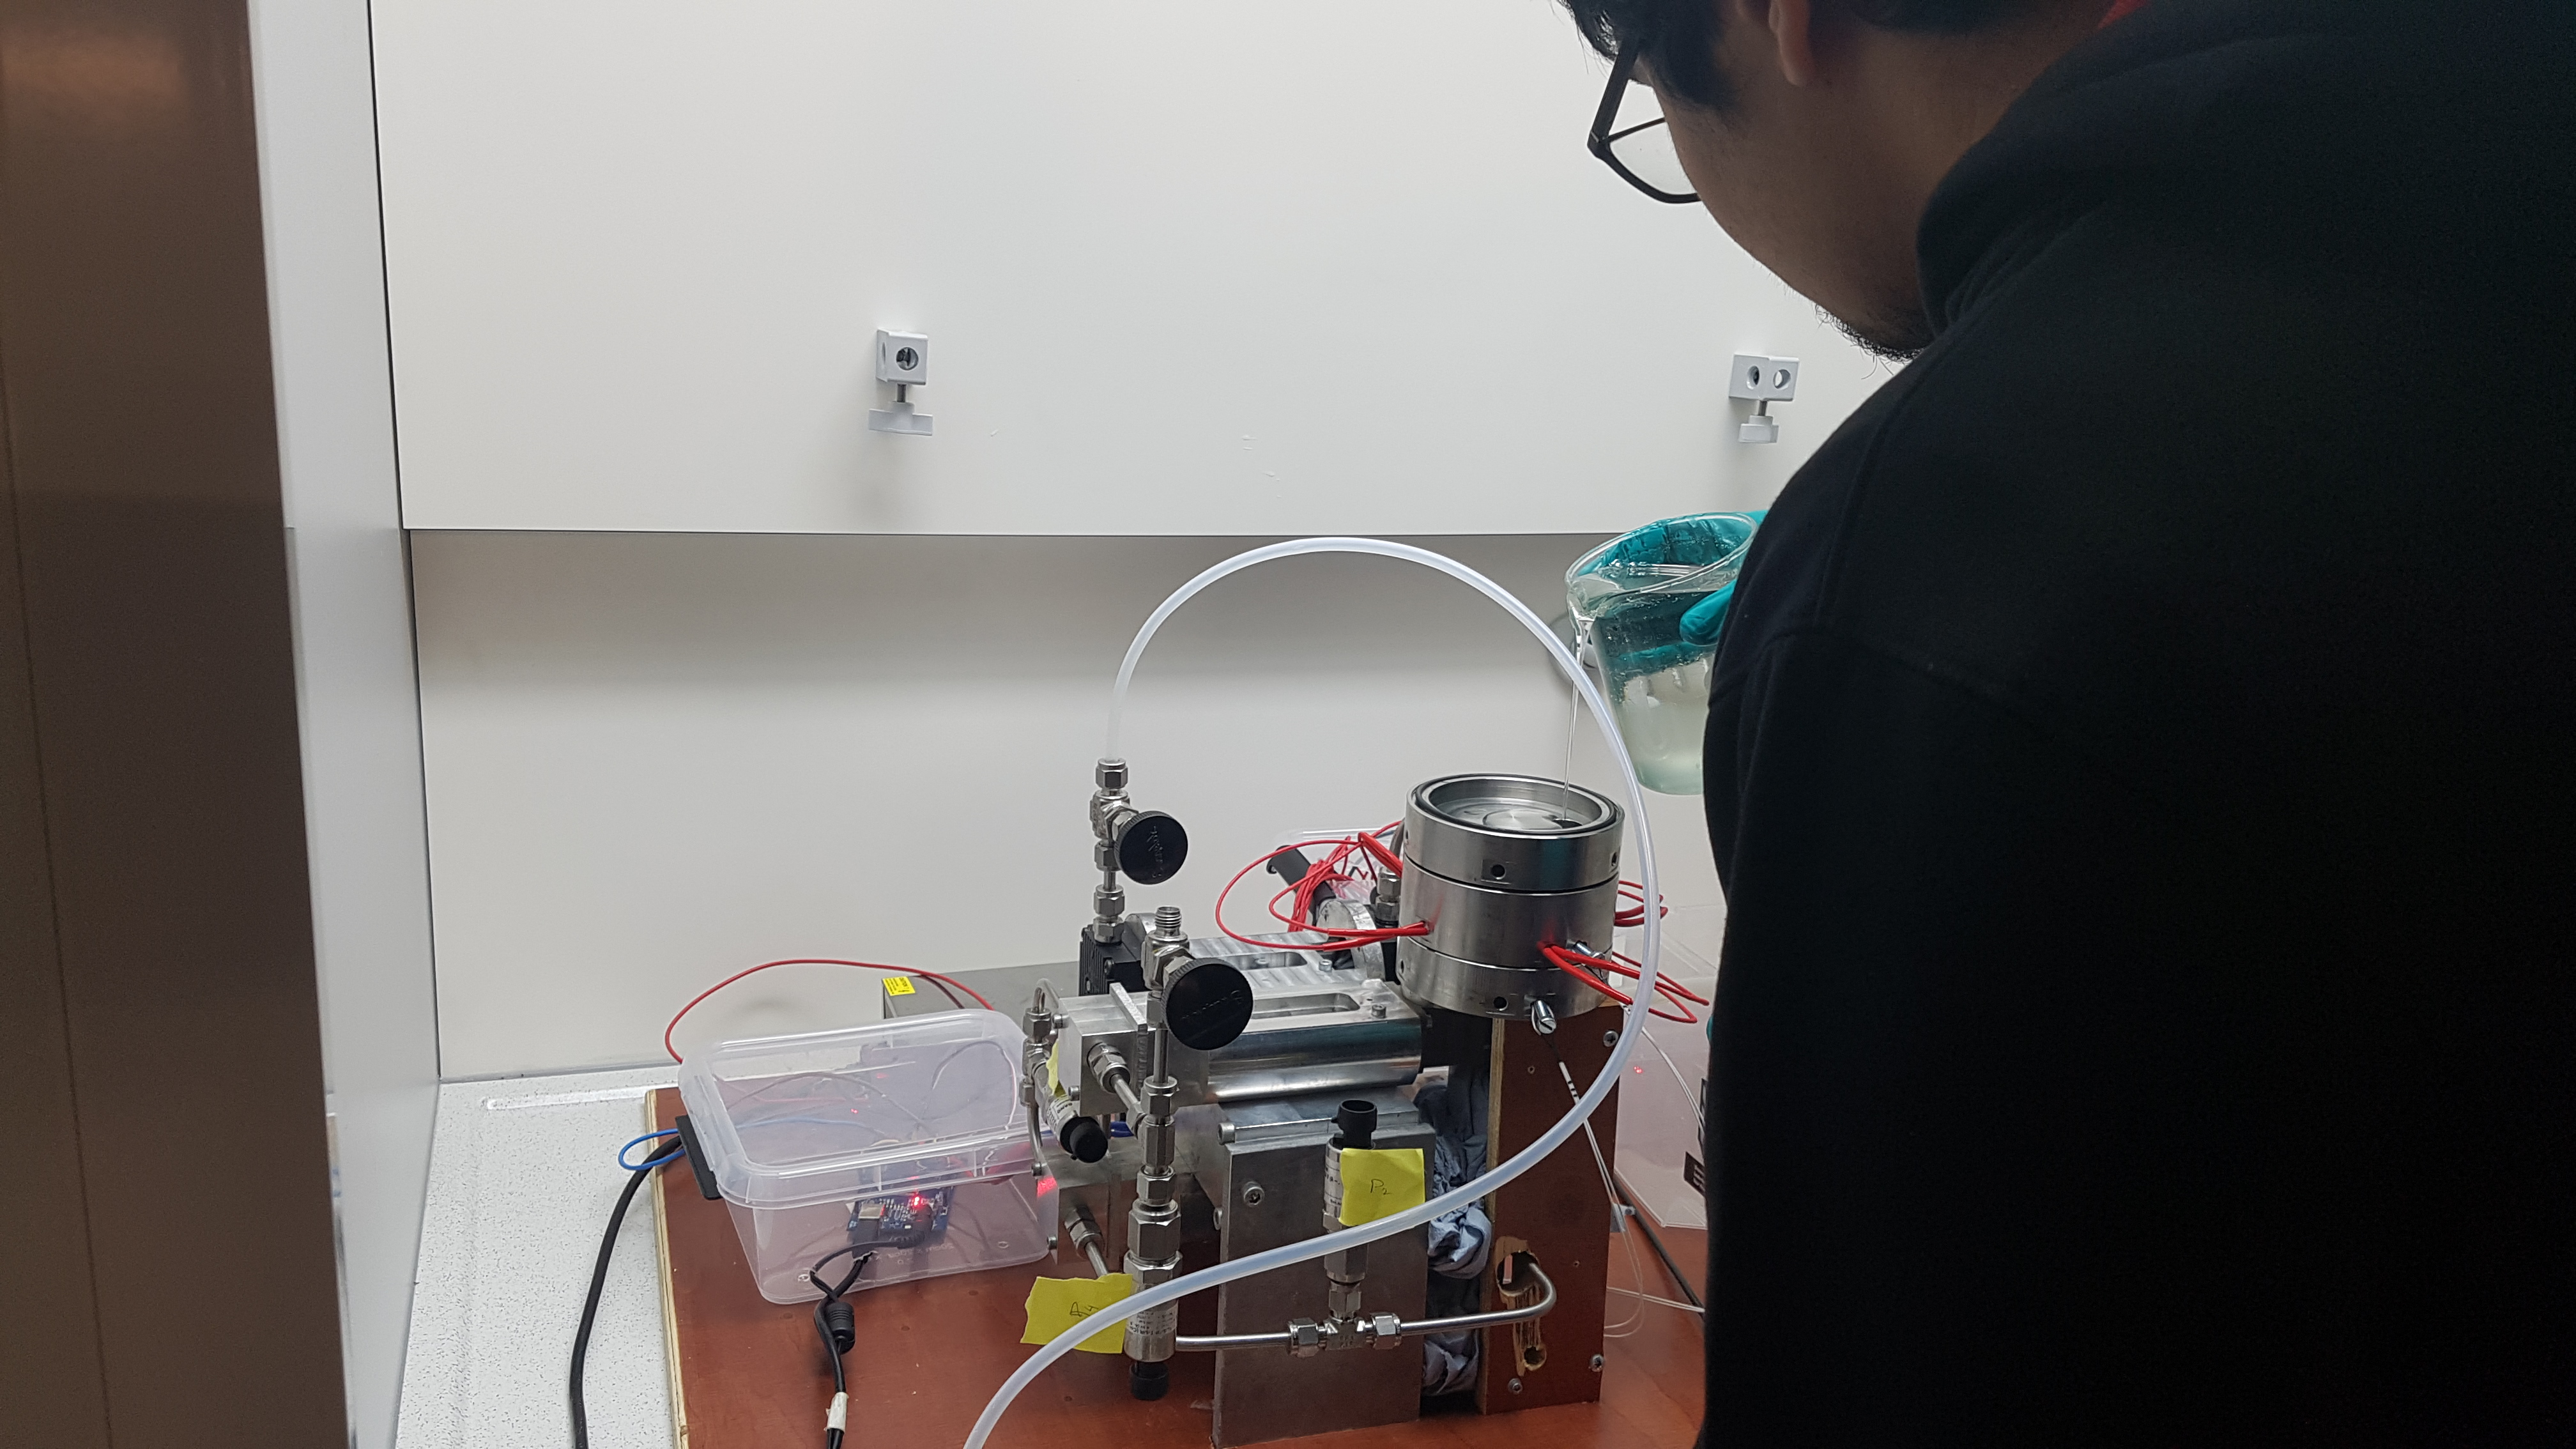
\includegraphics[scale = 0.09]{images/mywork/Sprint3/peiloading1.jpg}
    \caption{Loading PEI into the system}
    \label{fig:peiloading}
\end{figure}

It was observed that the PEI was so viscous that the PEI pump couldn't pump the normal PEI to the distributor. This was later inferred to be due to mainly two reasons :
\begin{itemize}
    \item Placement of the inlet nozzle in the extremes of the manifold - the inlet of the PEI flow from PEI pump to the DAC manifold was kept at the extreme nozzle. We know that there is significant pressure head loss when the length of pipe is very long. The solution for this was to cut the pipe length between DAC manifold and DAC distributor very short. The PEI inlet flow was shifted to the central nozzle as well for uniform distribution. 
    \item Using cold PEI - from previous reports we know that PEI becomes much less viscous at higher temperature. Hence, it wouldn't have much resistance in pumping the system up. 
\end{itemize} 


On rectifying the mistake and setting the heater temperature at 80 \degree C. The PEI was able to flow perfectly across the system and making it a continuous system. However, some observations were made that wasn't desirable which shall be elaborated more in the next Section of the report. 

\subsubsection{DAC System V1.1 breaks and issues}
\label{sec:breakdown}

During the entire runtime of the DAC System V1.1 we face many issues with broken 3D print components and leaks from the system. On further brainstorming and the cause of these issues and solutions were discussed. Some of the main issues that the system faced was : 

\begin{itemize}
    \item \textbf{Improper component geometry :} Due to improper design, improper assumptions and improper orientation. This can be seen in the following Figure \ref{fig:flowanomaly} below.
    \item \textbf{Desorber vibrations :} Due to improper orientation of the desorber chamber. At times, we could see that desorber would vibrate a lot out position and the chamber might come out of the vacuum condition. This caused a lot of PEI spills and was a pain to clean up as seen in Figure \ref{fig:leakingcompressor}. 
    
    \begin{figure}[H]
        \centering
        \begin{minipage}{.5\textwidth}
        \centering
        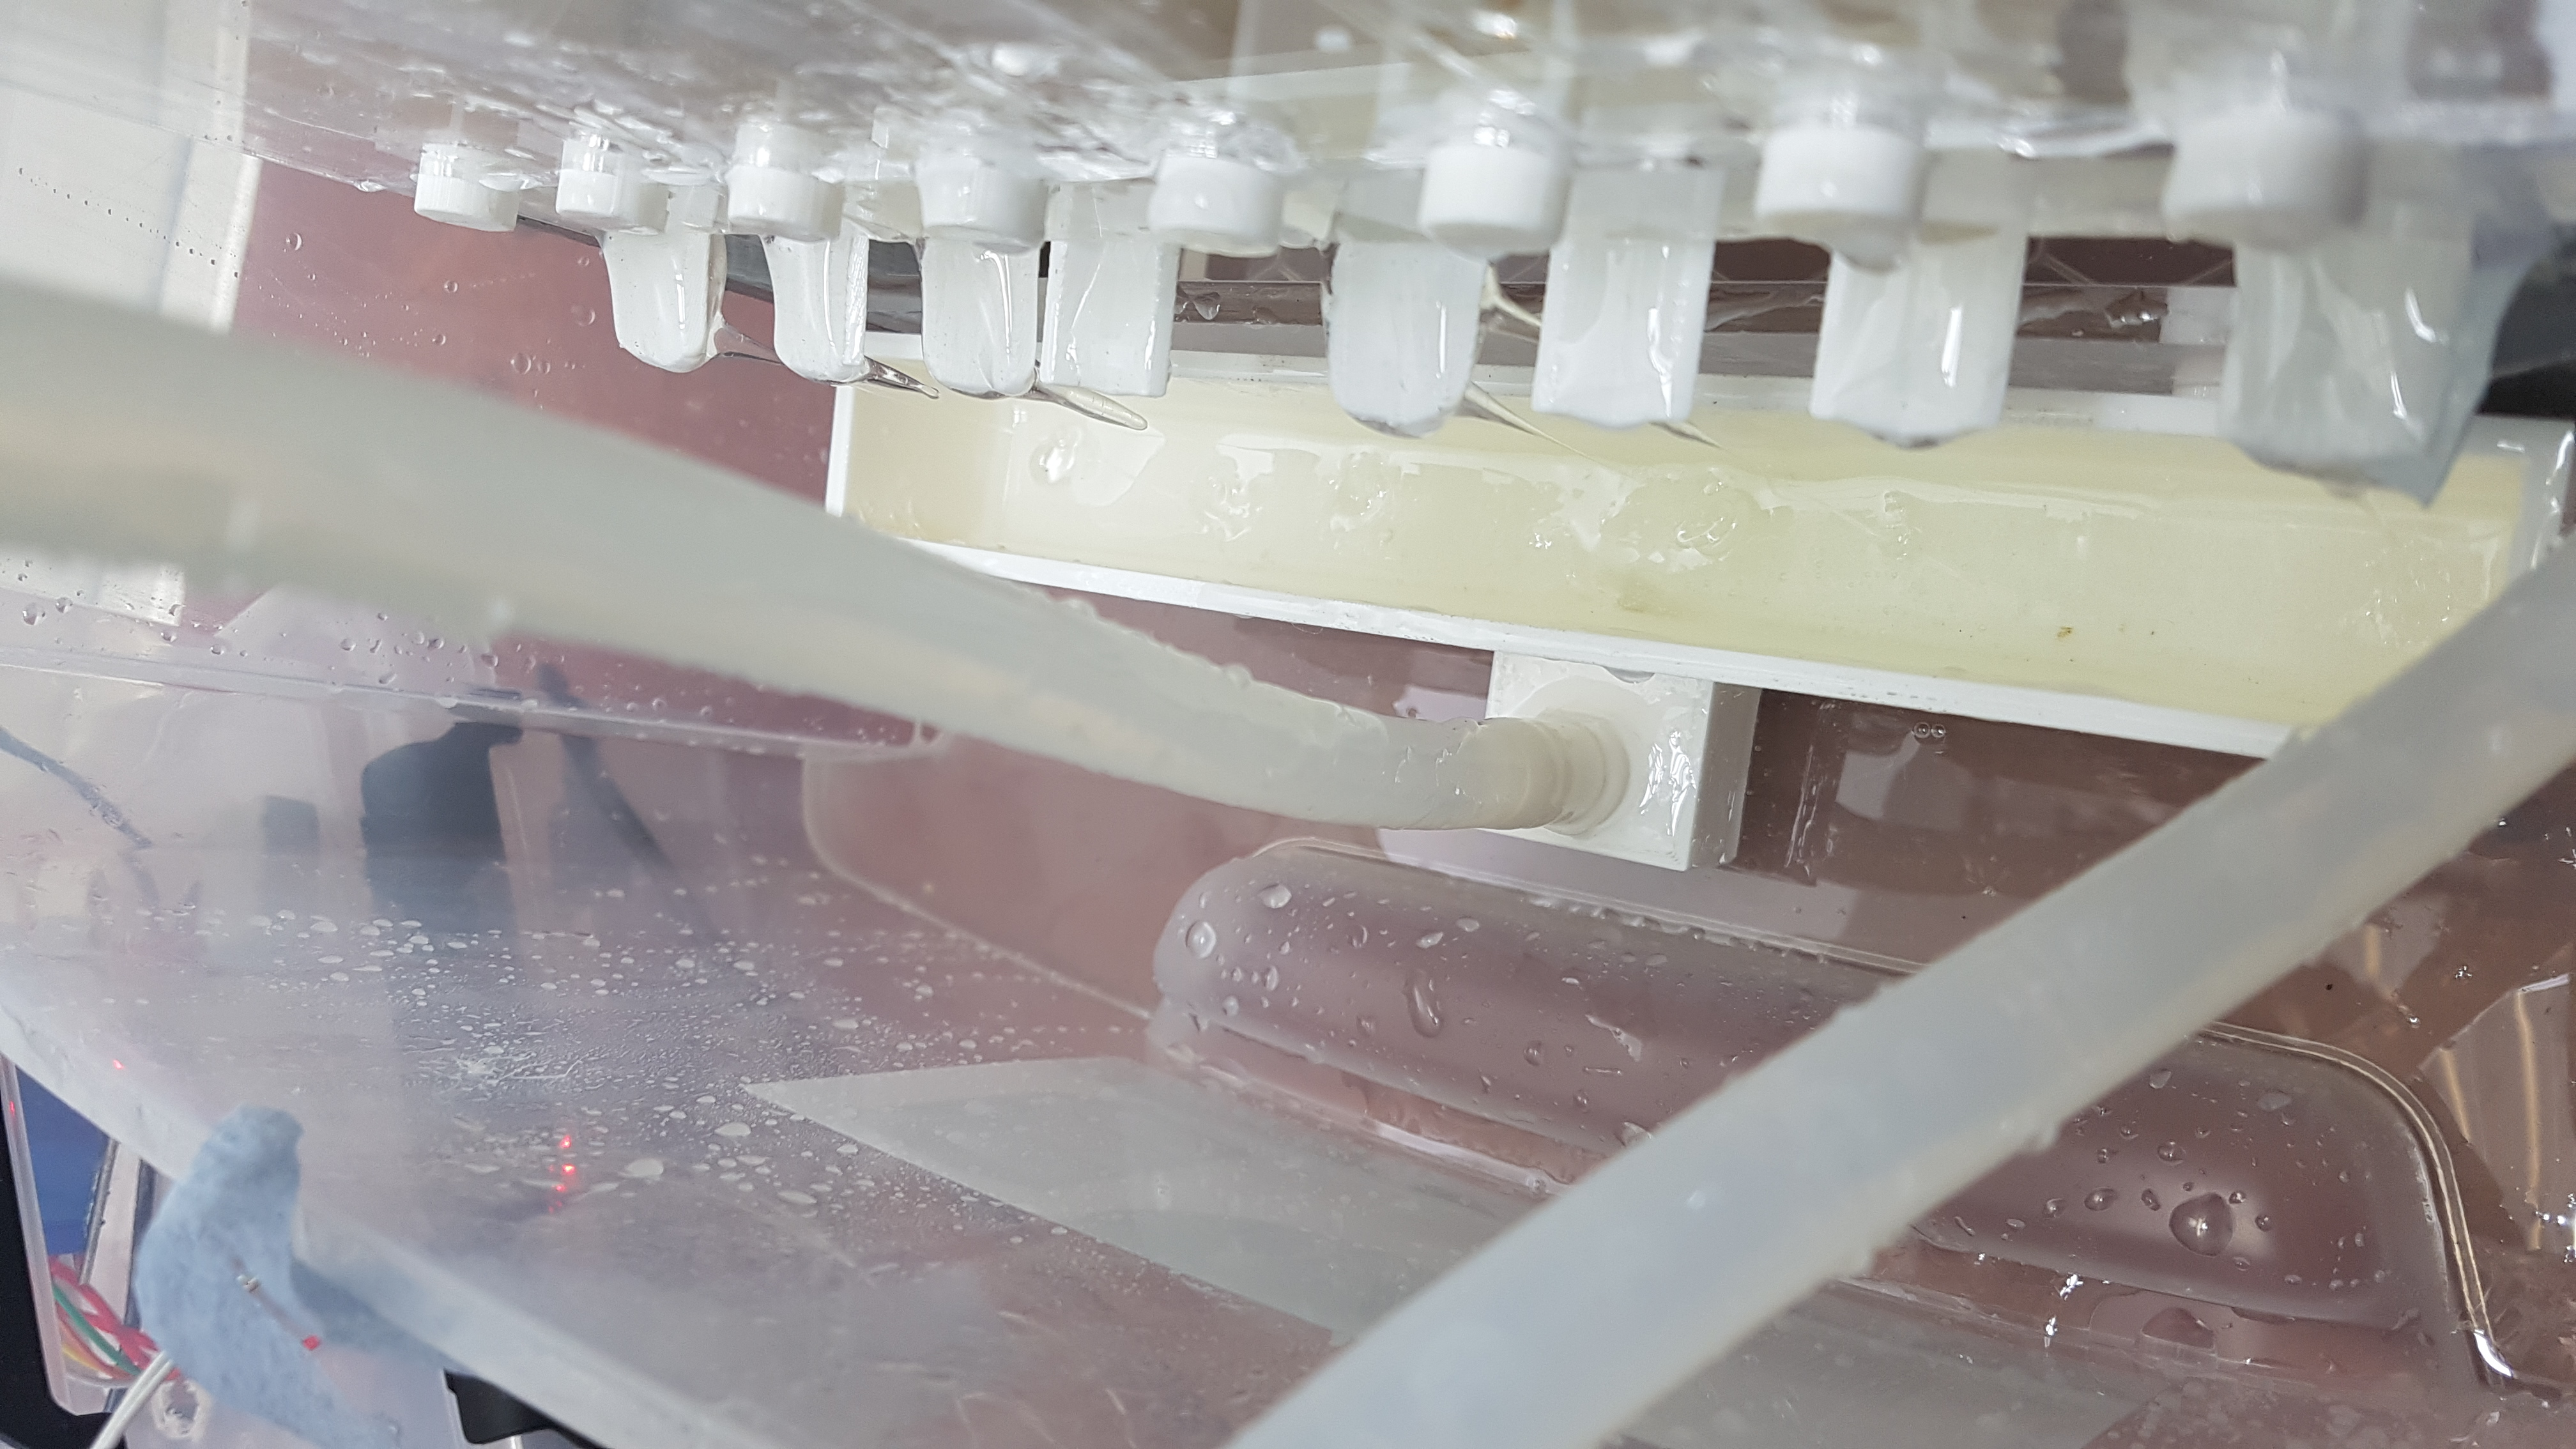
\includegraphics[width=0.9\linewidth, angle = 270]{images/mywork/Sprint3/flowanomaly.jpg}
        \captionof{figure}{Flow out of the DAC collector}
         \label{fig:flowanomaly}
    \end{minipage}%
    \begin{minipage}{.5\textwidth}
        \centering
        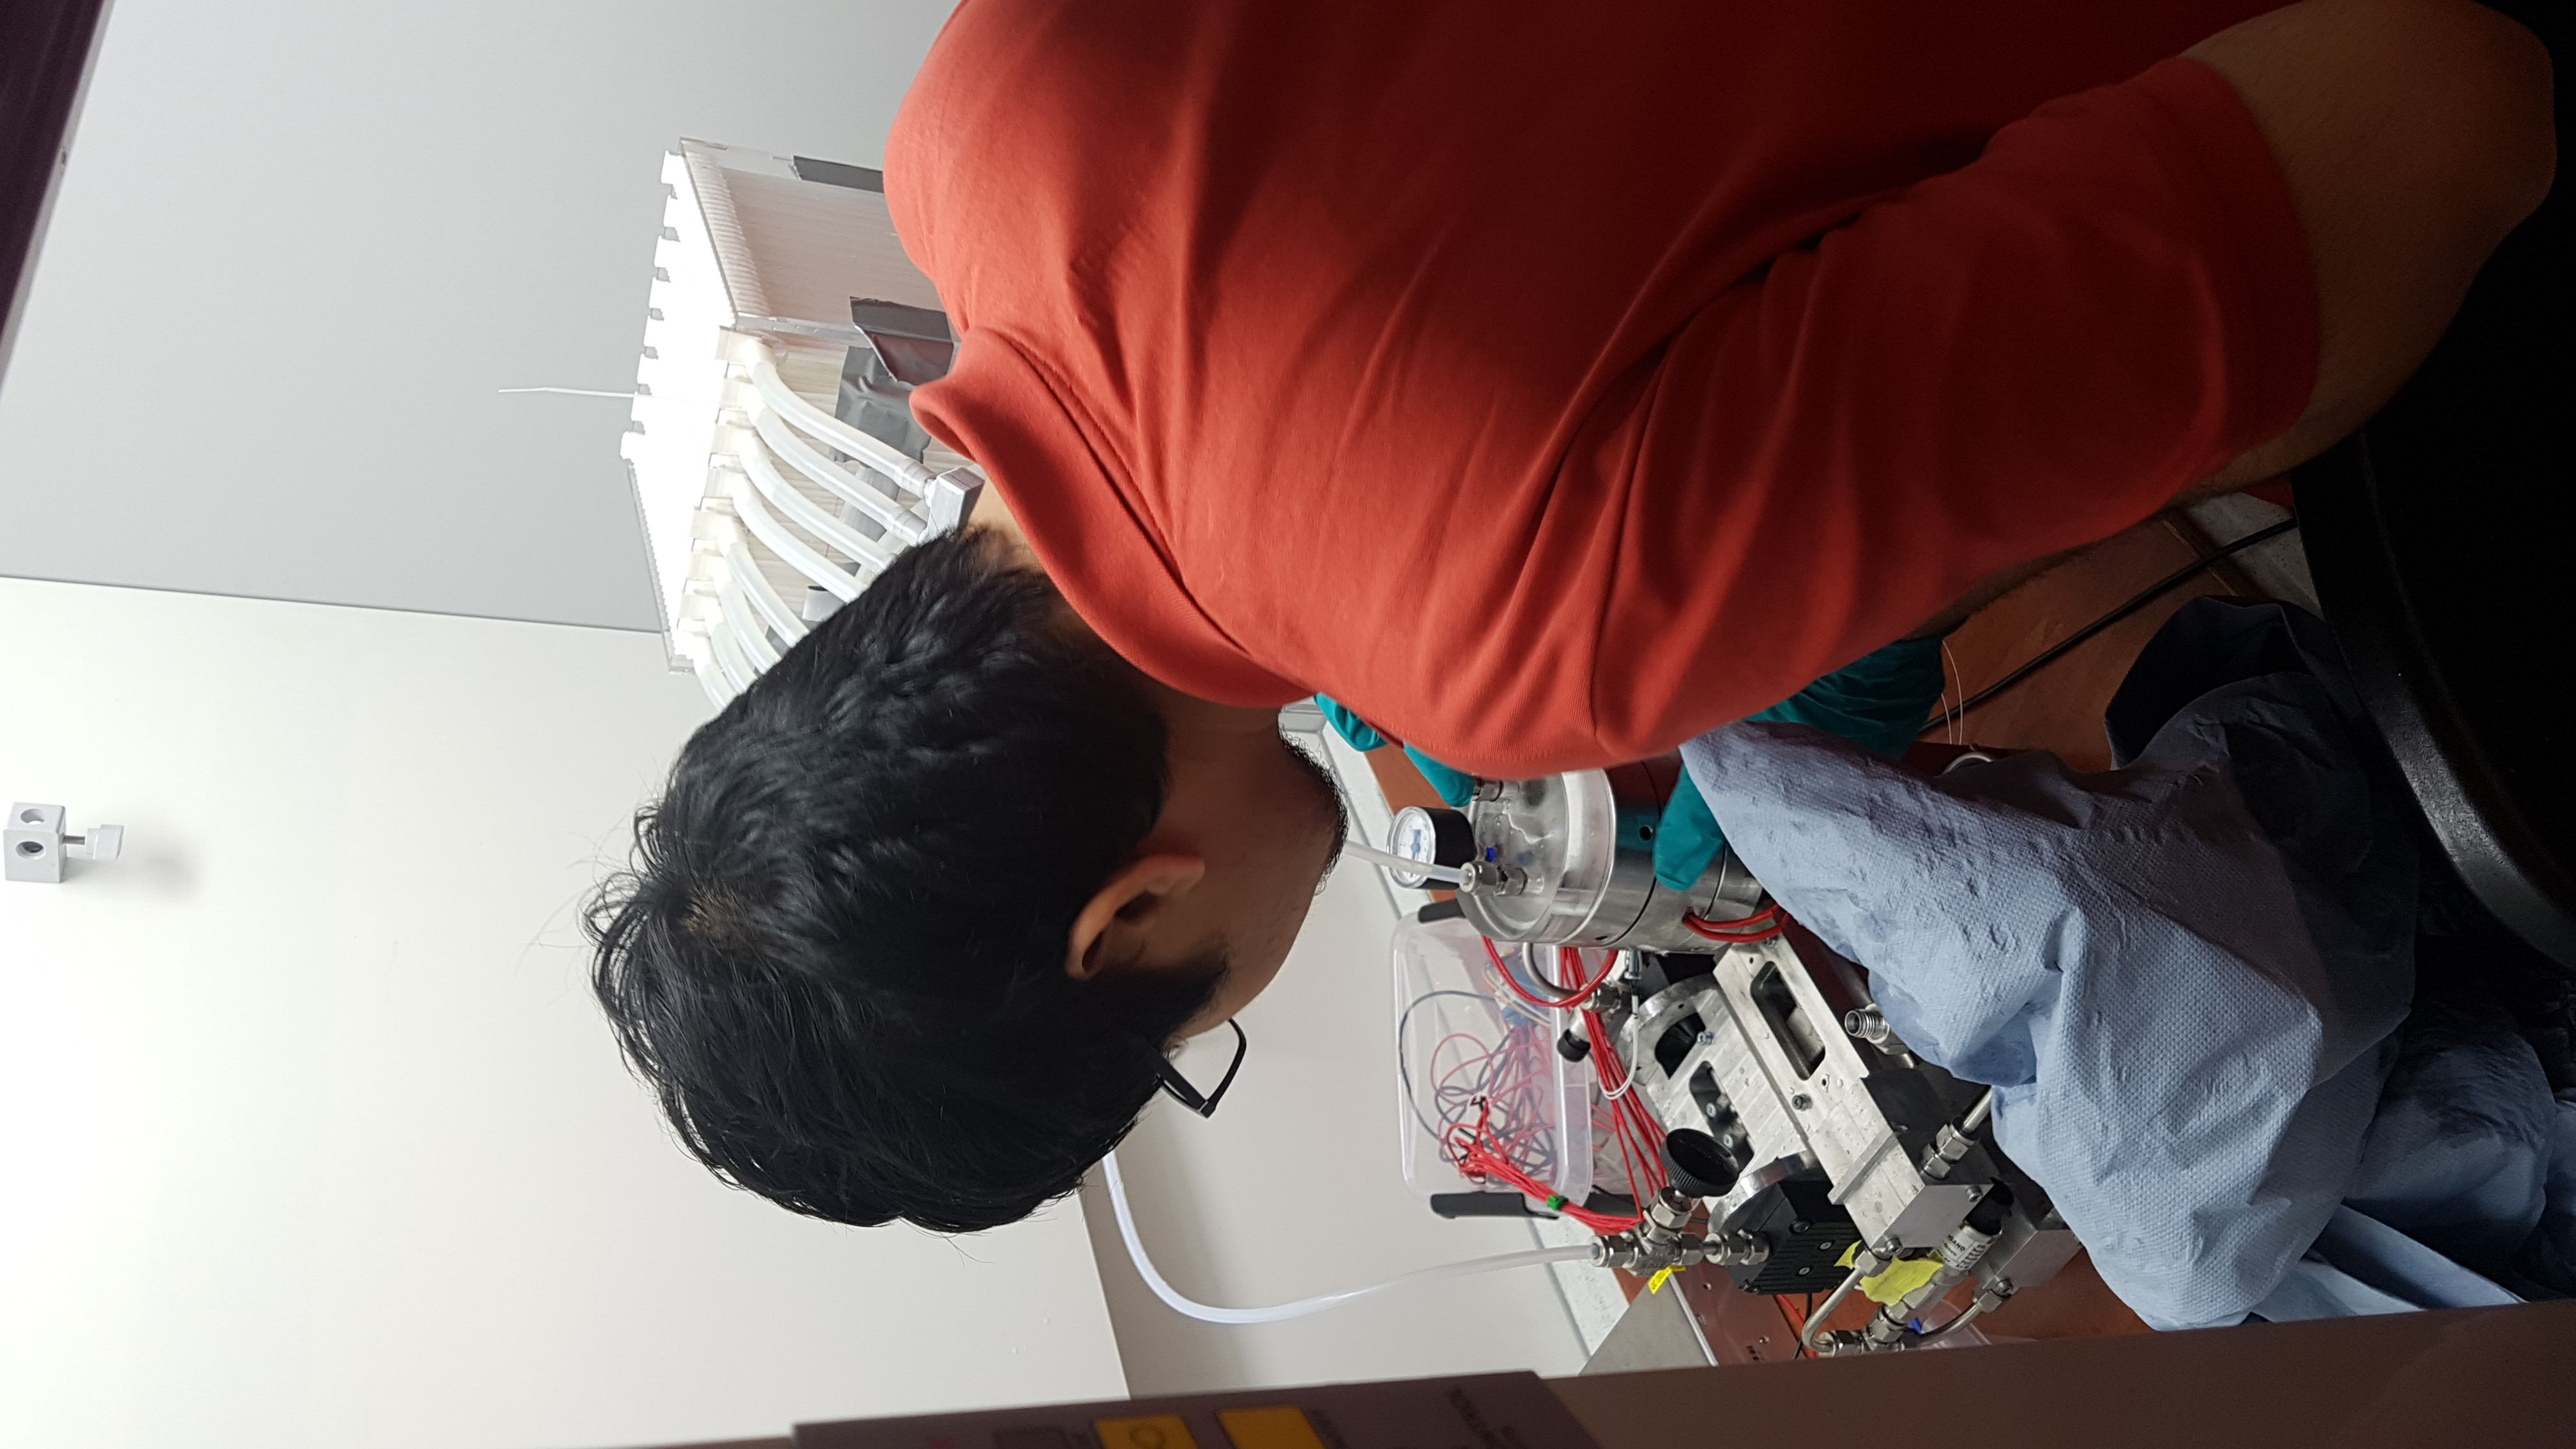
\includegraphics[width=0.9\linewidth, angle = 270]{images/mywork/Sprint3/messysystem.jpeg}
        \captionof{figure}{Leaking desorber chamber}
        \label{fig:leakingcompressor}
    \end{minipage}
    \end{figure}
    
    \item \textbf{Hot PEI reacts with PLA :}
    \label{sec:hotpei} During the Sprint 3 - a lot of our 3D prints were breaking like the collector bucket nozzle, the manifold nozzle and the distributor. At first, we inferred it was because of some accident or because of the way layers were set on the 3D printer making it a weak structure. However, on further studying it by putting a PLA piece in hot PEI. We found out that the PLA piece got completely dissolved within 30 minutes itself. Hence, it was decided that we have to look into other way to make the different DAC components.   
    
\end{itemize}


%copy paste from the section 3.3.1, section 3.3.2, section 3.4.1 and section 3.4 

\subsection{Observations from DAC V2.0 system}
\label{sec:DAC2.0}

Due to time constraints and as I was nearing the end of my internship. Further testing and running of the DAC V2.0 system was not possible. A few leak testing and tweaking the leaks were only done and has been explained below. The complete set up after assembly can be seen in Figure \ref{fig:dacv2.0} below. The labelled parts in the Figure is enumerated as per legend given below. 

\begin{enumerate}
    \item DAC V2.0 Distillation column 
    \item DAC V2.0 Absorber
    \item Vacuum pump
    \item Cooling finned tube
    \item Suction fan 
    \item DAC V2.0 Collector bucket
    \item Vacuum gauge
    \item DAC V2.0 Flowmeter
    \item T section and flashtank
\end{enumerate}

\begin{figure}[H]
    \centering
    \includegraphics[scale = 0.15]{images/mywork/Sprint5/dacv2.png}
    \caption{The DAC V2.0 system assembled}
    \label{fig:dacv2.0}
\end{figure}


\subsubsection{Vacuum leak testing}
\label{sec:DAC2.0leaks}

\noindent We found out that there is a leak in the system as the vacuum gauge wasn't staying steady once the vacuum pump was turned off. On isolating each part of the subsystem, we finalized that the issue was in the vacuum pump itself and we countered it by placing an On/Off valve right before the vacuum pump of the system. Hence, keeping the vacuum contained and operate the system in vacuum conditions. It was concluded that the leaks were mainly due to : 

\begin{itemize}
    \item Vacuum pump: It was found that there is were leaks present in the vacuum pump during vacuum testing. This is due to improper screwing in the male swageloke connectors. This made the leak testing difficult and was made the responsibility of the next ZEF team. 
    \item Distillation column: On vacuum leak testing the distillation column. We found that the vacuum pressure dropped to atmospheric pressure in a matter of few minutes. This indicated that there is leaks in the distillation column. On closer and detailed examination by leak testing each section of the distillation column. It was found that there were deep scratches in the bottom most stage. In order to overcome this, we had smoothened the surface out using sandpaper and by polishing it further using a DREMEL. 
    \item Reboiler \& Extra feed entry: Due to some improper welding for the swageloke connections. The vacuum couldn't be contained when the reboiler and extra feed entry in the distillation column were removed and tested seperately. Hence, they were welded again to avoid any such leaks. 
\end{itemize}




\newpage
\input{sections/discussion.tex}

\newpage
\section{Recommendations}
\label{sec:recom}

After spending three and a half months with the ZEF B.V and the DAC system. Some of the recommendations I have for the next team and ZEF B.V in general are in the following categories. I will cover what pre requiste knowledge would have been helpful for me during my internship. Then, I will cover some of the recommendations that I have for the DAC system and finally I would like to recommend some general recommendations for the ZEF VI that I think will be useful. 

\subsection{Pre requisite knowledge}

Before starting my internship at ZEF B.V and working on the DAC system. I wish I had knew the following things before starting my internship. Knowing these things beforehand would have increased my efficiency in performing my work on the DAC system. 

\begin{itemize}
    \item \textbf{Working with chemicals: }Coming from a background of mechanical engineering in my Bachelors and having irrelevant work experience. This was my first time working with chemicals such as PEI and TEPA. This led to some haphazard and careless handling with the chemicals that were harmful. It lead to making a mess of the workspace and making undesirable spills which could have been easily avoided if I had the chemical handling training. 
    
    \item \textbf{Arduino: }I had to spend a significant time learning about electronics and arduino as I didn't have a background in it. This could have been easily avoided if I knew beforehand that I will be working with arduino for pressure, temperature, level sensors and controlling other electronics. Although there was a arduino workshop by ZEF but it was too late as we already had started working on it. 
    
    \item \textbf{ZEF inventory: }It was never clear what items were under ZEF's inventory and there was never an inventory list in which we could check. This lead to asking DEMO and Michel for a lot of stuff that had to be accounted and returned as well. If I had known about the system before working on the system, it could have saved sometime and I could have generated ideas before starting my internship itself. 
\end{itemize}

\subsection{DAC System}

On working on two DAC systems at ZEF B.V. I had learnt a thing or two about working on the system such as the below points. 

\begin{itemize}
    \item \textbf{Chemical reaction: }As covered in this report about the DAC V1.1 system failure. It had never occured to test the reaction of PEI with PLA (3D printer material). If we had done this before starting the 3D printing of the DAC V1.1 system components. We could have easily ruled it out given the chemical degradation of PLA in PEI. This could have saved time and effort for ZEF B.V. Hence, considerable thought must be given during the conceptual design. 
    
    \item \textbf{PEI and TEPA behavior: }Inorder to understand why the DAC system had been designed as such. I would have liked to know more about the polyamines used in the DAC system. One possible solution is getting access to the ZEF reports by previous students well before the internship period.
\end{itemize}

\subsection{General recommendations}

Some general recommendations and advises that I have for the ZEF VI team is the following. 

\begin{itemize}
    \item \textbf{Not sure? Consult Jan: }Some of the errors that I had made during my internship could have been easily avoided if I had asked Jan when I wasn't sure about a process, design or anything at all. This lead to some careless mistakes that delayed the project unnecessarily. 
    
    \item \textbf{Taking delivery times into account: }We had a lot of downtime when we had to wait for the ordered parts. This lead to some downtime that I could have used for working on something else or helping in other system which in retrospect I should have done. It would have been a better utilization of my time in ZEF B.V. 
    
    \item \textbf{Writing report: }One thing I did right during my internship was writing the internship report simultaneously with the work I was doing in the internship. This lead to a detailed internship report and allowing me to work continuously on the DAC V2.0 system and the end of my internship when work was overloaded and not over working myself. I advice the further ZEFians to do the same as well.   
\end{itemize}


\newpage
\section{Conclusion}
\label{sec:conc}

As the growing concerns about global $CO_2$ emissions are now at all time high. Zero Emission Fuels B.V aims to address these concerns by designing and fabricating a micro plant. This micro-plant captures water vapour and carbon-dioxide from the atmosphere using a direct air capture (DAC) unit. The captured carbon-dioxide is then reacted with hydrogen that is generated from the captured water vapor from the alkaline electrolysis cell (AEC) unit of the micro plant to produced grade AA methanol that can be used in industries or as synthetic fuel in a methanol synthesis (MS) reactor.   
\bigbreak
\noindent
This report mainly focuses on the fabrication of the DAC unit of the ZEF micro-plant. Before designing and fabricating the DAC system, the previous iterations of the DAC unit were studied and noted down in Section \ref{sec:prework}. Based on these works, the new system was designed and fabricated which met with its own issues. This led to the fabrication of the new DAC V2.0 system which rectified this issues of the first system. However, due to constraints the setup couldn't complete testing and couldn't be run before the internship period. The design, component and process changes are all elaborated further in the report.    

\bigbreak
\noindent During the course of my internship in ZEF B.V. I have learnt a lot about LT DAC systems that have been utilized in the market at the moment and the ongoing research in the field. I was also able to engineer two LT DAC systems (DAC V1.1 system and DAC V2.0 system). Since, it was a interdisciplinary project that had a bit of everything. I had the immense pleasure of learning things that I had no experience such as working with chemicals, designing in fusion360, 3D printing and arduino programming. It also gave me the opportunity to work with a multi-cultural group that helped me understand a lot about the various cultures as well. 


\newpage
\bibliography{ref.bib}
\bibliographystyle{ieeetr}


\newpage 

\section{Appendix}
\begin{appendices}


\section{Arduino code}
\label{ap:arduino}

In this Section you shall see the Arduino codes that I used inorder to run some components of the DAC system. All the files will be available to you when requested. The following are the codes written for :

\subsection{Motor starting}
{\fontfamily{qcr}\selectfont
\#include<Servo.h> \\
\\
Servo myMotorFL; \\
\\
void setup() \\
\{ \\
 Serial.begin(9600); \\
 myMotorFL.attach(10); \\
 initialize\_motor(); \\
\} \\
\\ 
void initialize\_motor() \\
\{ \\
 Serial.print("Arming the motor!"); \\
 myMotorFL.write(40); //setting low RPM first \\
 delay(1000); \\
\} \\
\\
void loop() \\
\{  \\
  int val = 0;    // setting the motor at 40-130 RPM \\
  Serial.println(millis()); \\        
  myMotorFL.write(val); // letting the motor run at x RPM \\
  delay(1000); \\
\} \\
} \\

\subsection{PID Heater control}
{\fontfamily{qcr}\selectfont
\#include <ZEF.h> \\
ZEF\_ADS ADS;             	    // ADS board for NTC inputs \\
ZEF\_RELAYBOARD  RELAY(8,9);    	    // heater relays \\
ZEF\_PID\_CONTROLLER PID;             // PID heater control: to set PID values, use: ZEF\_PID\_CONTROLLER \\ PID(float Kp, float Ki, float Kd, float controlOutputMin, float controlOutputMax) \\
\\
int WindowSize = 1000;				// logging / control interval in ms \\
unsigned long WindowStartTime; \\
\\
int activeHeater = 0;				// the relay that is currently most active \\
float heaterRatioRelay0\_1 = 3/5;	// The ratio of heat cartridges of relay0 vs the total (relay0 + relay1) \\
float Output = 0; \\
float T\_NTC1, V\_NTC, T\_NTC2; \\
\\
void setup() { \\
\\
    //initialize modules \\
    ADS.begin(); \\
    RELAY.begin(); \\
    PID.begin(); \\
\\
    RELAY.setRelay(0,LOW); // turn relay 0 off \\
    RELAY.setRelay(1,LOW); // turn relay 1 off \\
\\
    Serial.begin(9600); \\
    Serial.setTimeout(50); \\
} \\
\\
void loop() { \\
    // check if window has ended, if so: update sensors, calc new PID output, \& log to serial \\
    if (millis() - WindowStartTime > WindowSize) \\
    { \\
        V\_NTC = ADS.readAbsoluteVoltage(1); \\
        T\_NTC1 = ADS.readNTCTemperature(1); \\
        T\_NTC2 = ADS.readNTCTemperature(2); \\
        Serial.print(millis()); \\
        Serial.print(","); \\
        Serial.print(T\_NTC1,2); \\
        Serial.print(", "); \\
        Serial.print(T\_NTC2,2); \\   
        Serial.println(); \\
\\
        // Calculate Control Output \\
        Output = PID.computeOutput(T\_NTC2); \\
\\
        // set base heater if necessary \\
        if (Output > heaterRatioRelay0\_1) \\
        { \\
            RELAY.setRelay(0,HIGH); \\
            activeHeater = 1; \\
            Output = (Output - heaterRatioRelay0\_1)/(1-heaterRatioRelay0\_1);		// Output adjust for 2nd heater scaling \\
        } \\
        else \\
        { \\
            RELAY.setRelay(1,LOW); \\
            activeHeater = 0; \\
            Output = Output/heaterRatioRelay0\_1;		// Output adjust for 1st heater scaling \\
        } \\
        // Reset window \\
        WindowStartTime = millis(); \\   
    } \\
\\
    // set heaters according to PID output \\
    test = millis()-WindowStartTime; \\
    if (test < Output*WindowSize){RELAY.setRelay(activeHeater,HIGH);} \\
    else {RELAY.setRelay(activeHeater,LOW);} \\
    \\
\\
    // Do communications \\
    checkCommunications(); \\
} \\
\\
void checkCommunications(){ \\
    // see if a command to change the setpoint has been received: \\
    if (Serial.available() > 0){ \\
            byte channel = Serial.read(); \\
            if(channel == 65){          //ASCII value of A \\
            // look for the next valid integer in the incoming serial stream: \\
            int command = Serial.parseFloat(); \\
                if (command>=0){ \\
                float newSetpoint = command; \\
                PID.newSetpoint(newSetpoint); \\
                Serial.print("\# Updated temperature SetPoint for Heaters: "); \\
                Serial.print(newSetpoint); \\
                Serial.println(" deg C"); \\
                } \\
            else{ \\
                Serial.flush(); \\
                Serial.println("\# invalid temperature SetPoint "); \\
                } \\
            } \\
    } \\
}  
}


\newpage
\section{MATLAB code}
\label{ap:MATLAB}

In this Section you shall see the MATLAB codes that I used inorder to evaluate some parameters for the DAC system. All the files will be available to you when requested. The following are the codes written for :

    \subsection{Hole size approximation}
    \label{sec:holesize}

    For calculating the actual hole size of the DAC V2.0 \bigbreak
    
    {\fontfamily{qcr}\selectfont
    
    \%\% Calculating the actual hole size \\

    \% Using paint and for the pixel sizing. \\
    \% I approximately calculated the actual size of the hole. \\
    \% I used a resistor wire which has a dia of 0.445 mm (using a micrometer) as reference \\
    \% Using coordinate geometry and ratios. The distance is calculated as follows. \\

    \%\% For the actual hole size calculation \\
    \%\% 

    \%for the resistor wire \\
    xr1 = 44; \%pixels \\
    yr1 = 63; \%pixels \\
    xr2 = 44; \%pixels \\
    yr2 = 50; \%pixels 
    drs = power((xr2 - xr1), 2) + power((yr2 - yr1), 2); \\
    dr = sqrt(drs); \%pixels \\
    act\_dr = 0.445; \%mm \\
    pix2mm = act\_dr/dr; \%mm/pixels \\

    \%for the resistor wire \\
    xh1 = xr2; \%pixels \\
    yh1 = yr2; \%pixels \\
    xh2 = 45; \%pixels \\
    yh2 = 17; \%pixels \\
    dhs = power((xh2 - xh1),2) + power((yh2 - yh1),2); \\
    dh = sqrt(dhs); \%pixels \\
    act\_dh = act\_dr + (dh*pix2mm); \\

    \%for 0.6mm hole, I am getting 0.9mm approx \\
    \%for 1mm hole, I am getting 1.5mm dia holes approx \\
    }
    
\subsection{Heat exchanger length calculation}


{\fontfamily{qcr}\selectfont
clc; \\
clear; \\

\noindent \%\% Assumptions \\

\noindent \%1. 10  mins to empty it all \\
\% 2. 1 and a half hour to fill 1.5 L \\
\% 3. Density not changing with T \\
\% 4. Cp not changing with T \\
\% 5. Check valve needed at the end, to prevent back flow \\
\% 6. All calculations are done as per - Pg. 62 - 77 for pin fin. \\
\\
\%\% Constants \\
\\
\% For PEI \\
CpPEI = 2000; \%J/kg-K \\
rhoPEI = 1270; \%kg/m3 \\
\\
\% For steel (Swageloke) \\
Ksteel = 502000; \%J/kg-K \\
\\
\% For steel pipe \\
di = 6*E-3; \%m  \\
do = 8*E-3; \%m \\
t = 1*E-3; \%m \\
\\
\% For Fin \\
Dfin = 0.01; \%m \\
lfin = 0.05; \%m \\
\\
\% Natural convection of air \\
h = 8; \%W/m2 - K \\
\\
\%\% Calculation of mass flow \\
\\
\% Assuming that it takes 1 hour to fill 1.5 L of PEI in the system \\
\\
VPEI = 1*E-3; \%m3 \\
tfill = 60*60; \%s \\ 
vdotPEI = VPEI/tfill; \%m3/s \\
mdotPEI = vdotPEI * rhoPEI; \%kg/s \\
\\
\%\% Heat to be removed \\
\\
Tdiff = 120 - 70; \%K, temperature difference between hot PEI and ambient air \\
Qdotremove = mdotPEI*CpPEI*Tdiff; \%W \\
\\
\% \%\% Fin parameters \\
\\
\% Afin = pi*Dfin*lfin; \\
\% Pfin = pi*Dfin; \\
\% beta = sqrt((h*Pfin)/(Ksteel*Afin)); \\
\\
\% \%\% Calculating heat dissipation \\
\\
\% Qdotdiss = Ksteel*Afin*beta*Tdiff*tanh(beta*lfin); \\
\\ 
\% \%\% Calculating number of fins needed \\
\\
\% nfin = Qdotremove/Qdotdiss; \\
\% X = beta*lfin; \\
\% efffin = tanh(X)/(X); \\
\\
\%\% Calculating length of straight finned tube \\
\\
\% Assumptions: \\
\% 1. Getting straight finned tube from Wino's contact \\
\% 2. Using 25.40mm base dia tube (1 inch) \\
\% 3. Using fin height of 9.55mm (the smallest one they have) \\
\% 4. Using fins per meter of 275 (the smallest one they have) \\
\% 5. Assuming fin thickness of 1mm \\
\\ 
\%Area of 1 fin \\
act\_bdia = 25.4*E-3; \%m \\
act\_hfin = 15.8*E-3; \%m \\
term1 = power((act\_bdia + act\_hfin),2); \\
term2 = power((act\_bdia - act\_hfin),2); \\
act\_Afin = 2*pi*(term1 - term2)/4; \%m2 \\
nfinperm = 275; \%no. of fins per m \\
\\
\%Heat dissipated from 1 fin \\
act\_Qdis = h*act\_Afin*Tdiff; \%W \\
\\
\%No. of fins needed for the complete heat dissipation \\
act\_nfin = Qdotremove/ac\_Qdis; \%no. of fins \\
\\
\%Length of the straight finned tube needed \\
act\_lfin = act\_nfin*100/nfinperm; \%cm \\
}



\newpage
\section{Fusion 360 drawings}
\label{ap:fusion}

\subsection{DAC V1.1 System}

\subsubsection{Distributor}

\begin{figure}[H]
    \centering
    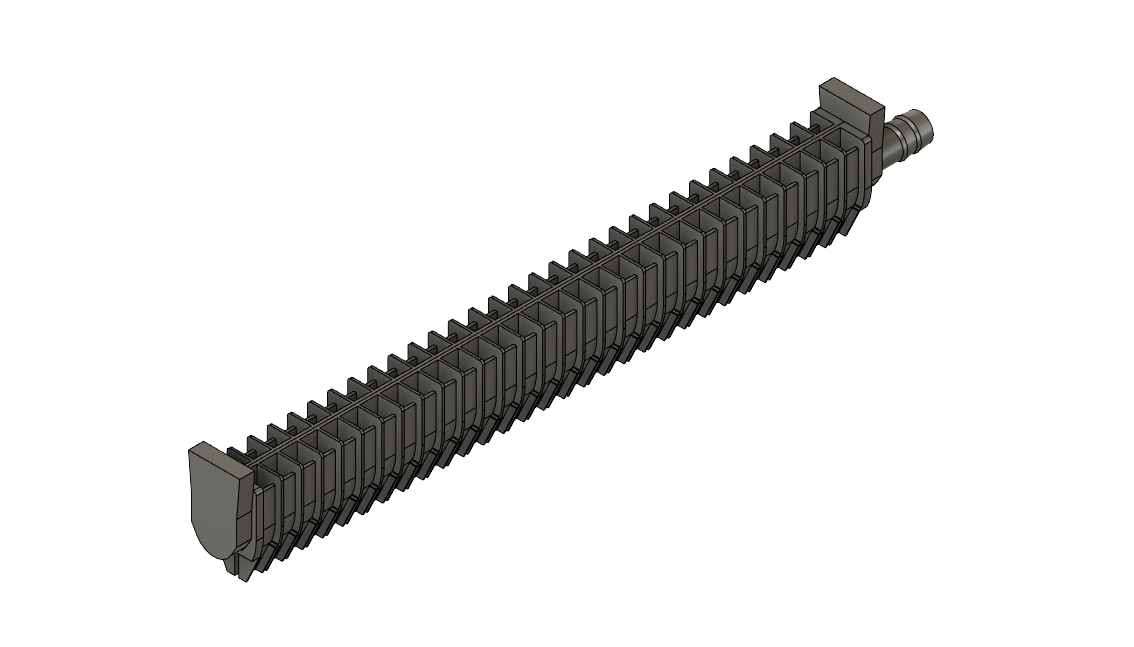
\includegraphics[scale = 0.4]{images/mywork/Sprint4/Distributor_old.png}
    \caption{DAC V1.1 Distributor}
    \label{fig:dacv1.1dis}
\end{figure}


\subsubsection{Manifold}

\begin{figure}[H]
    \centering
    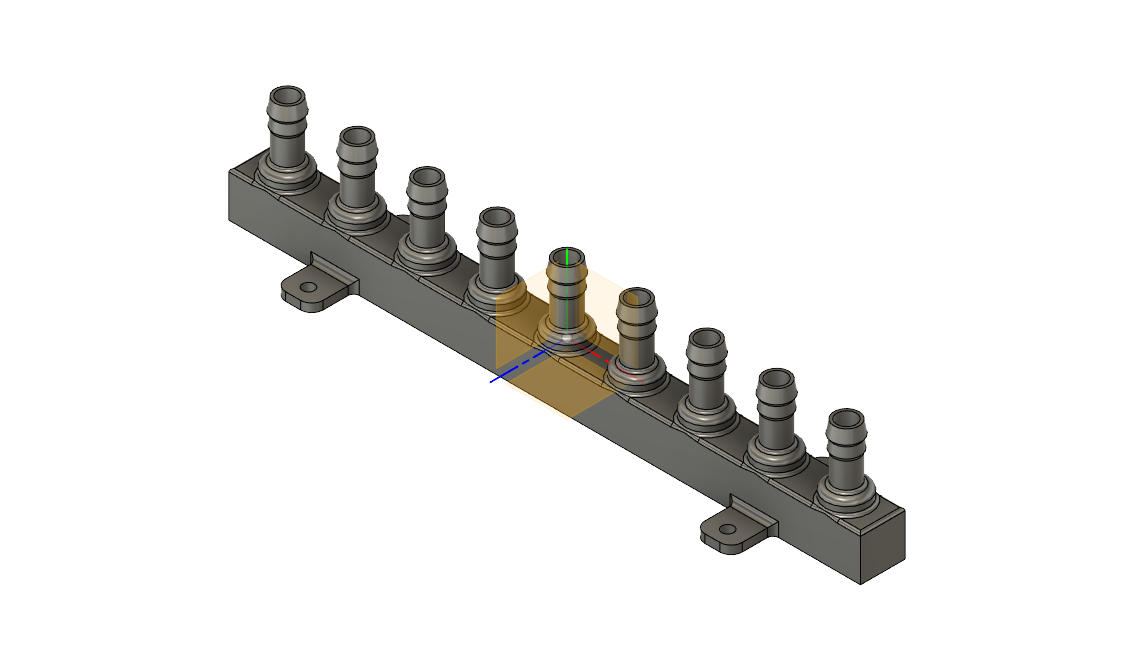
\includegraphics[scale = 0.4]{images/mywork/Sprint4/Manifold_old.png}
    \caption{DAC V1.1 Manifold}
    \label{fig:dacv1.1mani}
\end{figure}


\subsubsection{Collector}

\begin{figure}[H]
    \centering
    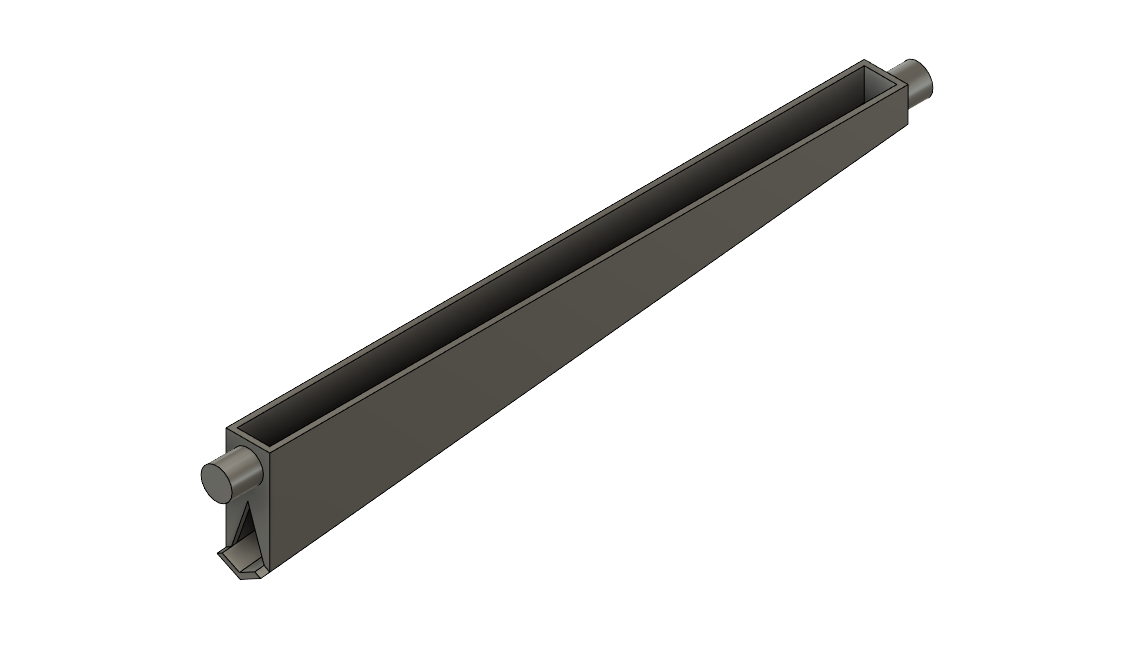
\includegraphics[scale = 0.4]{images/mywork/Sprint4/Collector_old.png}
    \caption{DAC V1.1 Collector}
    \label{fig:dacv1.1coll}
\end{figure}

\subsubsection{Collector bucket}

\begin{figure}[H]
    \centering
    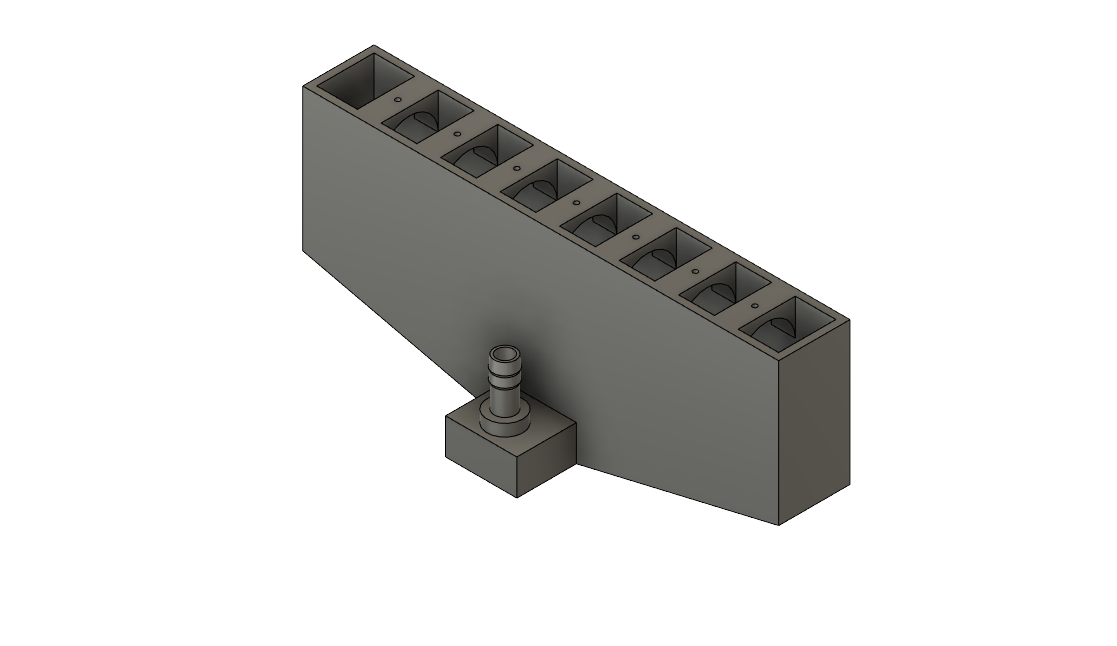
\includegraphics[scale = 0.4]{images/mywork/Sprint4/DACcollbuc_old.png}
    \caption{DAC V1.1 Collector bucket}
    \label{fig:dacv1.1collbuc}
\end{figure}



\subsection{DAC V2.0 System}

\subsubsection{Distributor}

\begin{figure}[H]
    \centering
    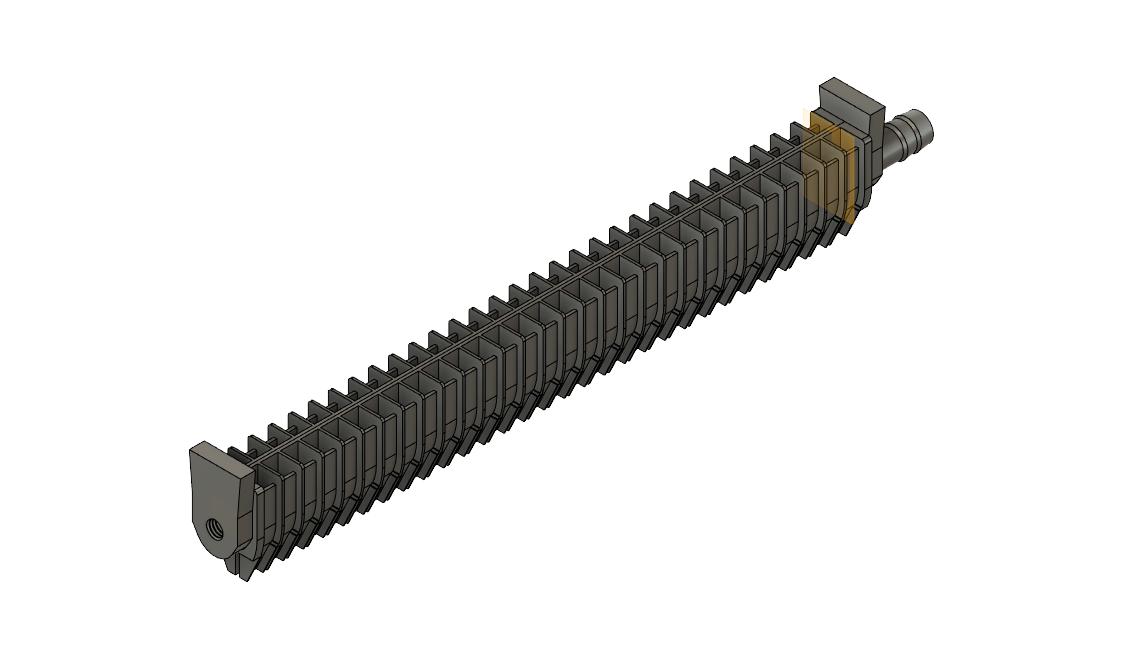
\includegraphics[scale = 0.4]{images/mywork/Sprint4/Distributor_main.png}
    \caption{DAC V2.0 Distributor}
    \label{fig:dacv2dis}
\end{figure}



\subsubsection{Manifold}

\begin{figure}[H]
    \centering
    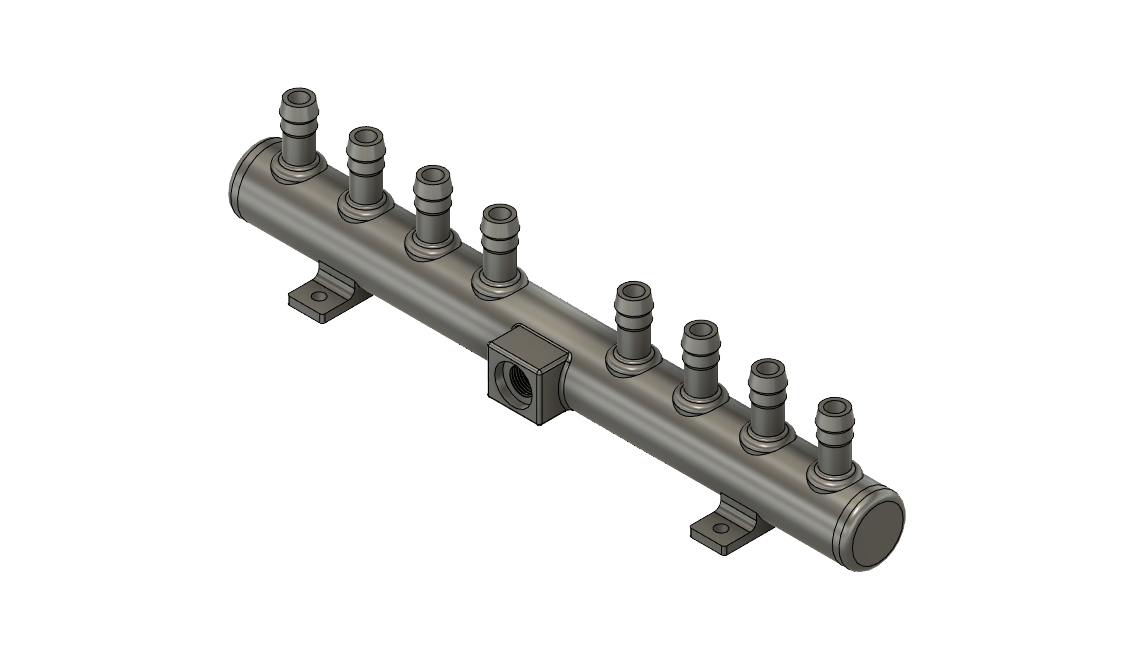
\includegraphics[scale = 0.4]{images/mywork/Sprint4/Manifold_main.png}
    \caption{DAC V2.0 Manifold}
    \label{fig:dacv2mani}
\end{figure}


\subsubsection{Collector}

\begin{figure}[H]
    \centering
    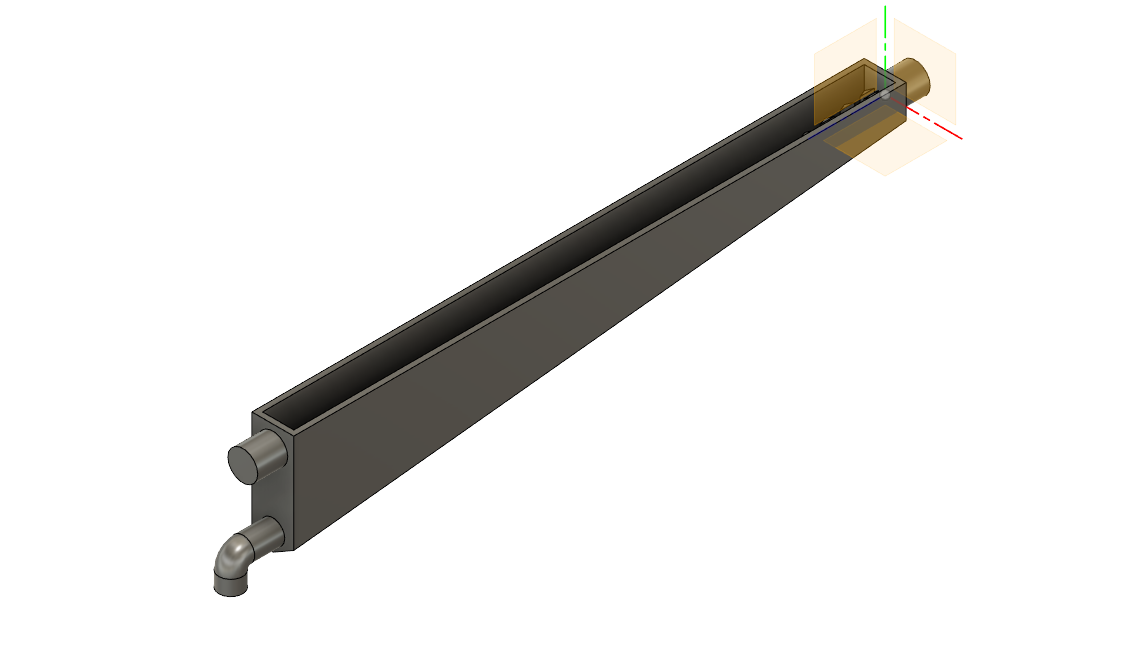
\includegraphics[scale = 0.4]{images/mywork/Sprint4/Collector_main.png}
    \caption{DAC V2.0 Collector}
    \label{fig:dacv2coll}
\end{figure}


\subsubsection{Collector bucket}

\begin{figure}[H]
    \centering
    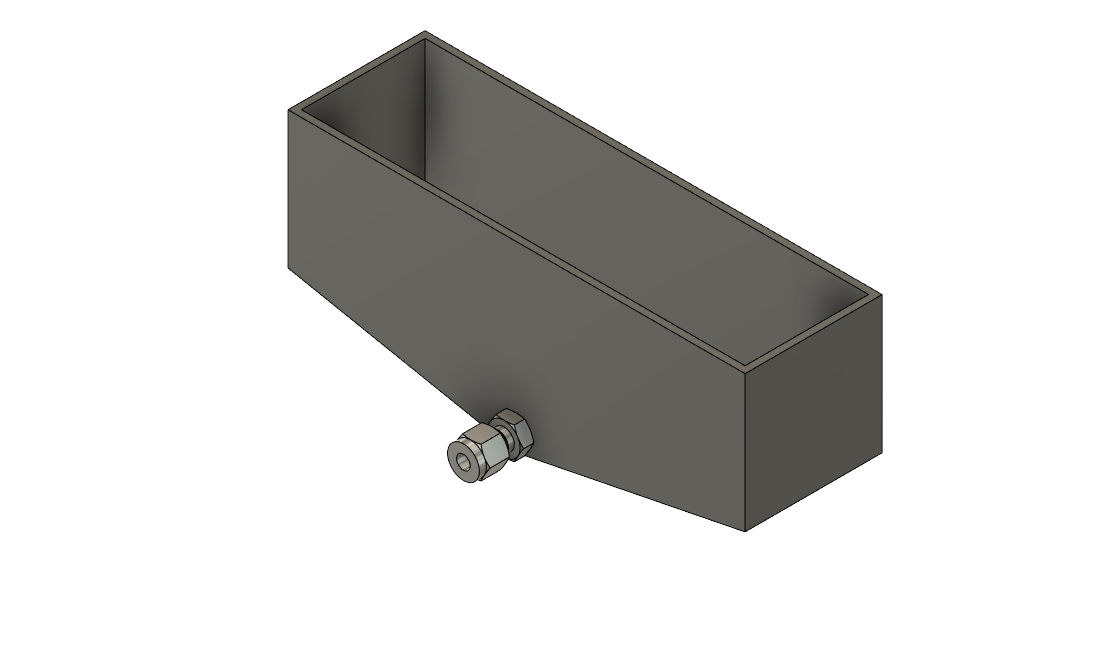
\includegraphics[scale = 0.4]{images/mywork/Sprint4/DACcollbuc_new.png}
    \caption{DAC V2.0 Collector bucket}
    \label{fig:dacv2collbuc}
\end{figure}


\subsection{The set - up}

\begin{figure}[H]
    \centering
    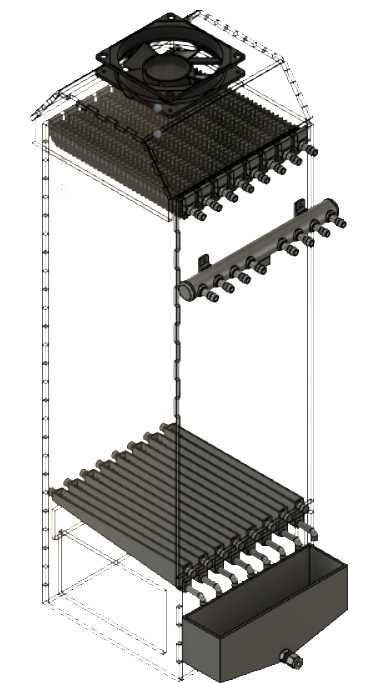
\includegraphics[scale = 1.4]{images/mywork/Sprint4/DACV2Absorber.png}
    \caption{DAC V2.0 Absorber}
    \label{fig:dacv2abs}
\end{figure}

\subsection{The complete set - up}
\label{sec:setup2.0}

\begin{figure}[H]
    \centering
    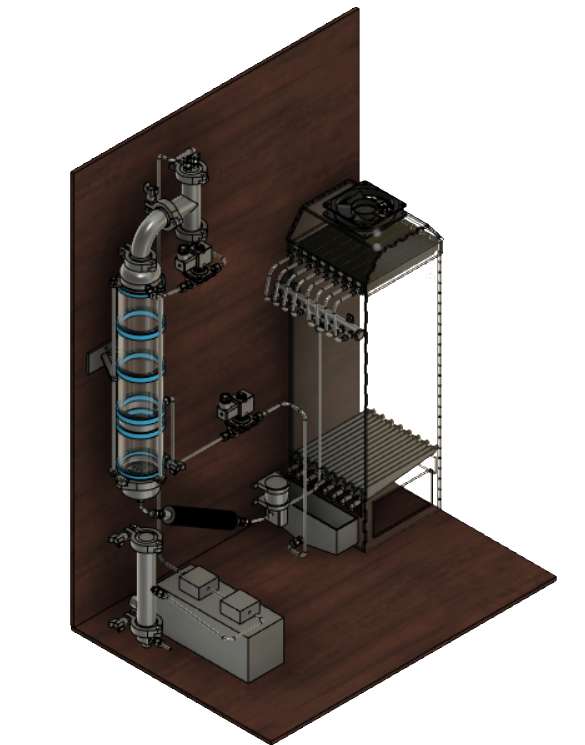
\includegraphics[scale = 1.4]{images/mywork/Sprint4/DACV2system1.png}
    \caption{DAC V2.0 System}
    \label{fig:dacv2system}
\end{figure}





\end{appendices}




%%%%%%%% EXTRA TIPS %%%%%%%%
%% hou deze structuur aan voor afbeeldingen
%%\begin{figure}[H]
%%\includegraphics[]{Pendulum.jpg}
%%\caption{Sketch of the pendulum}
%%\label{fig:pendulum}
%%\end{figure}


%%\newpage



\end{document}